\documentclass[preprint,review,12pt]{elsarticle}

\usepackage{amsmath}

\usepackage{amsfonts}
\usepackage{graphicx}
\newcommand{\Rho}{\mathrm{\textit{P}}}
\usepackage{subcaption}
\usepackage{csquotes}
\usepackage{algorithm} 
\usepackage{algpseudocode} 
\usepackage{longtable}
\usepackage[top=1.0in, bottom=1.0in, left=1.0in, right=1.0in]{geometry}
\begin{document}

\begin{frontmatter}

%% Title, authors and addresses

%% use the tnoteref command within \title for footnotes;
%% use the tnotetext command for theassociated footnote;
%% use the fnref command within \author or \address for footnotes;
%% use the fntext command for theassociated footnote;
%% use the corref command within \author for corresponding author footnotes;
%% use the cortext command for theassociated footnote;
%% use the ead command for the email address,
%% and the form \ead[url] for the home page:
%% \title{Title\tnoteref{label1}}
%% \tnotetext[label1]{}
%% \author{Name\corref{cor1}\fnref{label2}}
%% \ead{email address}
%% \ead[url]{home page}
%% \fntext[label2]{}
%% \cortext[cor1]{}
%% \affiliation{organization={},
%%             addressline={},
%%             city={},
%%             postcode={},
%%             state={},
%%             country={}}
%% \fntext[label3]{}

\title{Who You Gonna Believe, Me or Your Lying Eyes?\\
An Epidemiological Examination of Fake News and a Ranked Solution}

%% use optional labels to link authors explicitly to addresses:
%% \author[label1,label2]{}
%% \affiliation[label1]{organization={},
%%             addressline={},
%%             city={},
%%             postcode={},
%%             state={},
%%             country={}}
%%
%% \affiliation[label2]{organization={},
%%             addressline={},
%%             city={},
%%             postcode={},
%%             state={},
%%             country={}}

\author{By \\\textbf{John Hawthorne Smith} \\Thesis Project \\Submitted in partial fulfillment of the \\requirements for the degree of \\ \\MASTER OF SCIENCE IN DATA SCIENCE \\ \\Northwestern University \\February, 2021 \\ \\Nathaniel D. Bastian, PhD, First Reader \\TBD, Second Reader}

%\affiliation[Northwestern]{organization={Department One},%Department and Organization
%            addressline={Address One}, 
%            city={City One},
%            postcode={00000}, 
%            state={State One},
%            country={Country One}}

%\author[inst2]{Author Two}


\begin{abstract}
%% Text of abstract
TBD
\end{abstract}

%%Graphical abstract
%\begin{graphicalabstract}
%\includegraphics{grabs}
%\end{graphicalabstract}

%%Research highlights
%\begin{highlights}
%\item Research highlight 1
%\item Research highlight 2
%\end{highlights}

\begin{keyword}
%% keywords here, in the form: keyword \sep keyword
TBD \sep TBD
\end{keyword}

\end{frontmatter}

\tableofcontents

\section{Introduction}
\label{introduction}
\subsection{Background}
 In 2018, social media overtook print media as the fourth most popular source of news for Americans. As of 2019, 20\% "often" got their news from social media \cite{shearer2018social}, while 68\% of all American got their news from social media at least occasionally \cite{matsa2018news}. This is not inherently a bad thing - in countries with authoritarian leaders and state-run media, social media may be the only outlet for opposition spokespeople to share their messages \cite{walker2014breaking}; ordinary citizens can now contribute their stories and experiences without the high financial barrier to entry that traditional journalism requires \cite{qualman2012socialnomics, tapscott2008wikinomics}; in unmanageable situations and crises, such as the 2017 Manchester bombing, social media allows for the instantaneous exchange of information between individuals and emergency management agencies \cite{mirbabaie2020breaking, eriksson2016facebook}; in situations like the COVID-19 pandemic, where information is rapidly evolving, social media allows for immediate knowledge dissemination by dramatically shortening the traditional time from publication to widespread translation to adoption \cite{chan2020social}. Furthermore, experts can readily reach followers who may not have deep knowledge of a subject - Dr. Esther Choo, a strong science communicator who writes for \textit{The Lancet} and frequently appears on \textit{NBC} and \textit{CNN}, has over 113,000 followers – and can increase awareness of public health needs and crises, while openly debating other experts and answering direct questions \cite{gottlieb2020information}.

However, not all information shared on social media is true, and the subset of people who primarily get their news from social media tend to be less engaged, less knowledgeable of current events, more likely to hear unproven claims and conspiracy theories than those who get their news from more traditional sources, and are more likely to believe these conspiracies \cite{mitchell2020americans}. In just two examples of this, Edgar Maddison Welch drove from North Carolina to Washington D.C. with an AR-15 to investigate a fake pedophile conspiracy ring known as "pizzagate" in December 2016, \cite{goldman2016comet}; in 2018, Burmese officials created over 1,000 Facebook posts filled with hate speech and detailing fake crimes committed by the Rohynga Muslim minority to justify one of the largest forced migrations in recent history \cite{subedar2018country}.

Exacerbating this problem, the spread of correct information is much slower than that of misinformation: while true rumors tend to be validated within 2 hours of the first tweet, false rumors take about 14 hours to be debunked \cite{zubiaga2016analysing,shao2016hoaxy}. This is a problem since, in a crisis event, 50\% of all retweets occur within the first hour after a tweet is shared and 75\% are within the first day \cite{kwak2010twitter}. Even if an untrue story is debunked, corrective information does not reach as broad of an audience as misinformation does \cite{maddock2015characterizing, vosoughi2018spread}, and, in some cases, rumors and other fake stories actually see an increase in spread \textbf{after} they have been debunked \cite{starbird2014rumors}. In the case of the "pizzagate" conspiracy, several news outlets -- including \textit{The Washington Post}, \textit{The New York Times}, and Snopes -- had debunked the story several months before Welch decided to drive to Washington D.C. \cite{kang2016fake,lacapria2016fact,board_2016}, yet pro-conspiracy posts on Facebook, Instagram, YouTube, and Twitter actually saw a sharp uptick as the supporters became more zealous post-debunking\cite{kang2016washington}. In fact, this fits a pattern where highly controversial and politicized topics spark backfire effects when passionately held misconceptions are challenged \cite{gollust2009polarizing,nyhan2010corrections,nyhan2013hazards,redlawsk2010affective,schaffner2016misinformation,hart2012boomerang}.

At a very high level, this thesis seeks to balance this dilemma. If the viral spread of misinformation can be curbed before it reaches overzealous partisans, then the backfire effects and deadly scenarios can be avoided. 

\subsection{Problem Statement}
\label{Problem Statement}
A reasonable person might still question at this point why this is a problem that needs solving. There is nothing fundamentally new and original about lying, especially on controversial or political topics. While this is true, it is imperative not to sink into an \textit{argument from inertia} fallacy \cite{bennett2012logically} and suggest that because history has survived this issue in the past, there is no reason to improve in the present. Arguably, there are three major reasons to try to prevent the spread of fake news: the legal, the ethical, and the humanitarian.

\subsubsection{Legal Objection to Fake News}
In 2014, 27 states prohibited false statements regarding elections \cite{Vasilogambros2019political}. While some of those states have had their laws reduced or reversed in the past 6 years, others have scaled up their laws regarding misinformation. One of the key results of Vol I of the Mueller Report was the indictment of "13 Russian nationals and three Russian entities—including the Internet
Research Agency (IRA) and Concord Management and Consulting LLC (Concord)—with violating U.S. criminal laws in order to interfere with U.S. elections and political processes" \cite{mueller2019mueller,mueller2020internet}.

While it is true that the US Supreme Court has routinely ruled in favor of providing more freedom than less when it comes to speech, false statements with dire consequences do not fall under those rulings. In the US Supreme Court Ruling in 2012 on \textit{United States v. Alvarez}, the Court built on previous cases protecting First Amendment rights for even unsavory speech such as  \textit{Ashcroft v. ACLU 2002}, \textit{Ashcroft v. ACLU 2004}, \textit{Brandenburg v. Ohio}, and \textit{United States v. Stevens} by stating: 
\begin{quote}The remedy for speech that is false is speech that is true. This is the ordinary course in a free society. The response to the unreasoned is the rational; to the uninformed, the enlightened; to the straight-out lie, the simple truth.\cite{scotus2012alvarez}\end{quote} 
However, in that decision, the Supreme Court drew a distinction between false speech for falsity's sake and cases where there is demonstrable harm attached to the false statements such as in \textit{Hustler Magazine, Inc. v. Falwell}, \textit{Brown v. Hartlage}, \textit{Virginia Bd. of Pharmacy, supra}, \textit{Herbert v. Lando}, \textit{Gertz, supra}, and \textit{Garrison v. Louisiana}. In \textit{Garrison v. Louisiana}, the Court unequivocally stated "[T]he knowingly false statement and the false statement made with reckless disregard of the truth, do not enjoy constitutional protection" \cite{scotus1964garrison} and in \textit{Hustler v. Falwell}: "[f]alse statements of fact are particularly valueless [because] they interfere with the truth-seeking function of the marketplace of ideas" \cite{scotus1987hustler}. 

While this thesis makes no pretense of being a legal brief or an analysis of constitutional law, it is valuable to confirm that the goal of this thesis is not fundamentally unconstitutional or illegal. In fact, the cited quote from \textit{Hustler v. Falwell} is the guiding principle of this thesis: it is not the intention of this thesis to remove bad ideas from the marketplace, but to remove bad faith ideas.

\subsubsection{Ethical Objection to Fake News}
In book one of \underline{Metaphysics of Morals}, Immanuel Kant argued that the great injustice of lying is that it robs the person being lied to of the freedom to make their own decisions \cite{kant1996metaphysics}. By operating with an incomplete or incorrect set of facts, a virtuous and rational person could make an unethical and misguided decision that they would not have made otherwise. This is not dissimilar from the arguments made in the Mueller report and in the indictment against the IRA: Count One was "conspiracy to defraud the United States" in order to interfere in the 2016 election  \cite{mueller2019mueller,mueller2020internet}. The primary goal of the IRA, per Mueller, was to sow confusion -- getting individuals to accept the fraud was a bonus -- and make people unsure of which sources, if any, they could trust. That goal was successfully met as 64\% of Americans believe that fake news causes a great deal of confusion and roughly 1 in 4 admit to having shared fake stories themselves \cite{barthel2016americans}. Those rates of confusion are relatively consistent across the political spectrum, gender, income levels, etc. 

One example of a Russian fraud account is @TEN\_GOP (fig. \ref{fig:Russian Troll Account @TEN_GOP}), \begin{figure}[h]
    \centering
    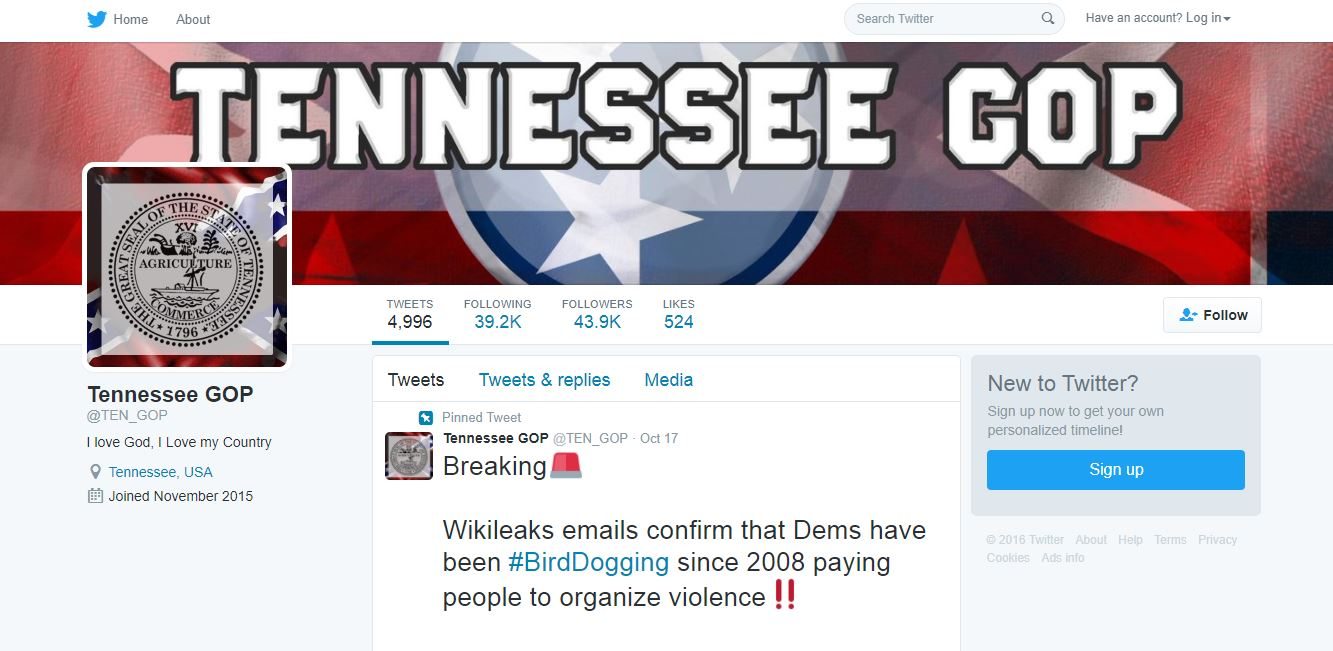
\includegraphics[width=11cm]{Ten_GOP.jpeg}
    \caption{@TEN\_GOP, Russian Troll Account}
    \label{fig:Russian Troll Account @TEN_GOP}
\end{figure} which is mentioned repeatedly in the Mueller report and claimed to be the official twitter of the Tennessee Republican Party. It racked up over 100,000 followers and frequently shared false information regarding voter fraud which was then retweeted by multiple individuals key to the Trump campaign, such as Donald Trump Jr., Eric Trump, Kellyanne Conway, Brad Parscale, and retired General Michael Flynn \cite{mueller2019mueller}. As will be discussed later in \ref{Partisanship Section}, individuals will conform to the opinions of the rest of a group, even if it runs contrary to their personal convictions or facts they've personally observed \cite{asch1956studies}, especially in politically charged environments \cite{bullock2007experiments,housholder2014facebook}. In this case, since the misinformation was being amplified and effectively cosigned by key political figures, rank-and-file Republicans believed @TEN\_GOP's fraud. This is the heart of the ethical objection: while incendiary opinions and statements may evoke strong polarized responses, 
the viral spread of misinformation intends, at its core, to exploit human weakness, gaslight its recipients, and rob them of the freedom to make informed decisions.


\subsubsection{Humanitarian Objection to Fake News}
\label{Humanitarian Objection to Fake News Section}
The humanitarian arguments are the most important reasons for curbing the spread of disinformation. In previous sections, the "pizzagate" story where a person brought an AR-15 into a restaurant was discussed, but this is far from a unique example. Hours after the 2013 Boston Marathon Bombing, members of social media hypothesized that an innocent Brown University student was behind the attack \cite{starbird2014rumors}; he committed suicide shortly after. A father of a child who was killed during the 2012 Sandy Hook shooting was harassed by social media members convinced that the shooting was a hoax \cite{williamson2019alex}; he too committed suicide shortly after. On September 9 2020, a conspiracy theory began that the fires in Oregon were started by the left-wing activist group called Antifa \cite{robinson2020oregon}; on September 11th, the FBI put out a statement declaring the reports untrue \cite{fbi2020portland}; on September 12th, Facebook began removing these untrue posts; weeks later, Oregon officials were still wasting resources that should have been going towards firefighting to handle the non-stop deluge of calls and emails about the rumor \cite{wilson2020oregon}. Most recently, on January 6, 2021, incited by the former President of the United States's debunked claims over election fraud and a baseless internet conspiracy group called Q-Anon, a mob broke into the U.S. Capitol and threatened to execute members of Congress and the Vice President \cite{fandos2021trump}; five people were killed directly from riot \cite{Levenson2021capitol}.

Not all misinformation leads to active cases of violence. Misinformation exacerbated the Ebola epidemic in West Africa \cite{shultz2016role}, interfered with measles vaccination efforts \cite{hussain2018anti}, and disrupted health policies and procedures during the current COVID-19 pandemic \cite{bagherpour2020covid,world2020novel,zarocostas2020fight,depoux2020pandemic,habersaat2020ten,van2020using}. Groups that were fed misinformation downplaying the severity of COVID-19 saw a higher lack of compliance with safety measures -- such as mask wearing and social distancing -- and a higher number of cases and deaths \cite{bursztyn2020misinformation}. Even though the United States has seen numerous days of more than 4,000 deaths due to the virus, only half of the country is currently planning on getting a vaccine when it's available \cite{cornwall2020just}. The misinformation content has run the gamut from misleading messages about the actions or policies of public officials \cite{brennen2020types}, to suggesting the vaccine is a conduit for Bill Gates to inject microchips into people \cite{sanders2020difference}, to blaming 5G cell towers \cite{jolley2020pylons,goodman2020coronavirus}, to inciting people to vandalism \cite{spring2020coronavirus}, to, in some cases, promoting mob violence and mass poisonings \cite{depoux2020pandemic}. Even if the final violent example is stripped away, the potentially unchecked spread of deadly disease is cause enough for concern. 

\subsubsection{Summary}
\label{misinformation summary}
To summarize, misinformation is not protected by the First Amendment, is ethically wrong, and can have life-or-death consequences. This thesis does not seek to root out every misstatement, ill-thought out opinion, and dubious political attack ad. Instead, it is only focused on content that could provide a clear threat to election integrity, human life, etc. This limited scope is fundamentally different from the approaches taken by other recent literature on the topic, and will be discussed further in Sec. \ref{sec: literature review}.

\subsection{Fake News Definition}
\label{Fake News Definition Section}
Before continuing, it's important to get a clear definition of what is meant by the term "fake news". The primary and most frequently cited definition of fake news comes from Allcott \& Gentzkow: "[they are] articles that are intentionally and verifiably false, and could mislead readers" \cite{allcott2017social}. Several existing studies adopt this definition \cite{conroy2015automatic,klein2017fake,rubin2015deception,rubin2017deception,mustafaraj2017fake,potthast2017stylometric}, and most attempt to parse out the further differences between \textit{misinformation}, \textit{disinformation}, \textit{rumor}, \textit{fake news}, etc. \cite{zimdars2020fake,  difonzo2007rumor,flynn2017nature,garrett2013undermining,wu2016mining}. Wu et al. provide the following diagram of their proposed parsing:
 \begin{figure}[htp]
    \centering
    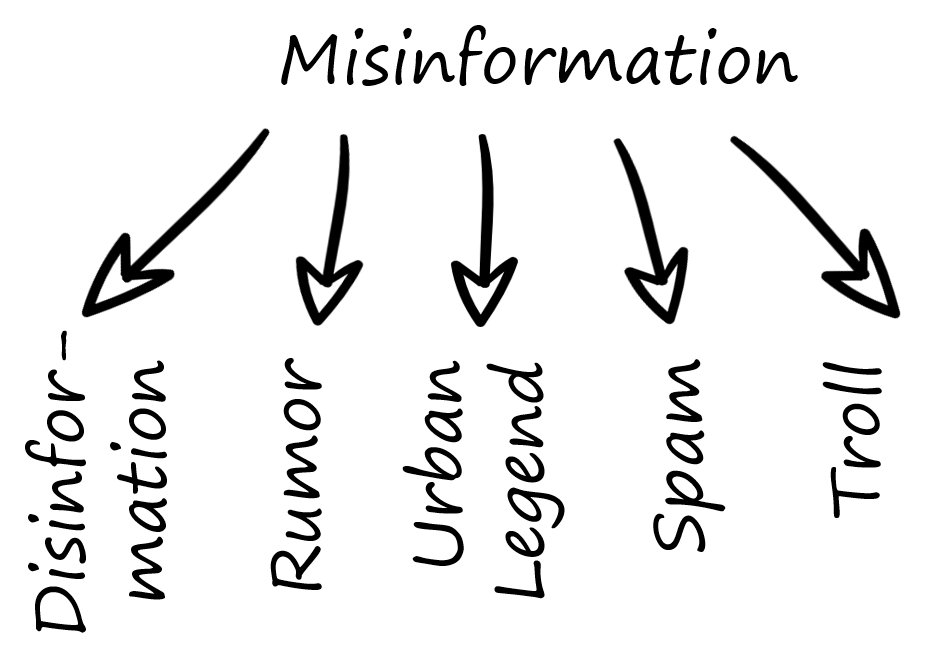
\includegraphics[width=4cm]{misinformation graphic.png}
    \caption{Misinformation Labels \cite{wu2016mining}}
    \label{fig:misinformation graphic.png}
\end{figure}


The dividing line between most of these categories is the level of intentionality: e.g. \textit{misinformation} is false but the creator has no verifiable  intent to mislead the reader, whereas \textit{disinformation} is false and the creator has a high intent to mislead the reader, and \textit{rumors} may be true or false, but the truth value is currently undetermined.

This has lead to an alternative definition from Klein \& Wueller: "[misinformation is] a news article that is intentionally and verifiably false". \cite{klein2017fake}. This definition has seen growth and has also been accepted by current studies \cite{shu2017fake, liu2018early}.

To bridge this gap, a more epistemological approach is proposed. For every tweet $t$ in the set of tweets $T$, there is a corresponding truth value $\tau$ between 0 and 1 (0 means something is completely false and 1 means something is completely true):
\begin{equation}
\label{truthvalues}
    \forall \ t \in T \ \exists \ \tau, \tau \in \mathbb{R} \ | \ 0 \leq \tau \leq 1
\end{equation}
Several previous works on this topic set $\tau \in \ \{0,1\}$ \cite{liu2018early,shu2017fake}. This is incorrect, as statements may be false, partially true, mostly true, or completely true. For example, this tweet from conservative provocateur Charlie Kirk (fig. \ref{fig:Charlie Kirk Tweet, May 4, 2020})  \begin{figure}[h]
    \centering
    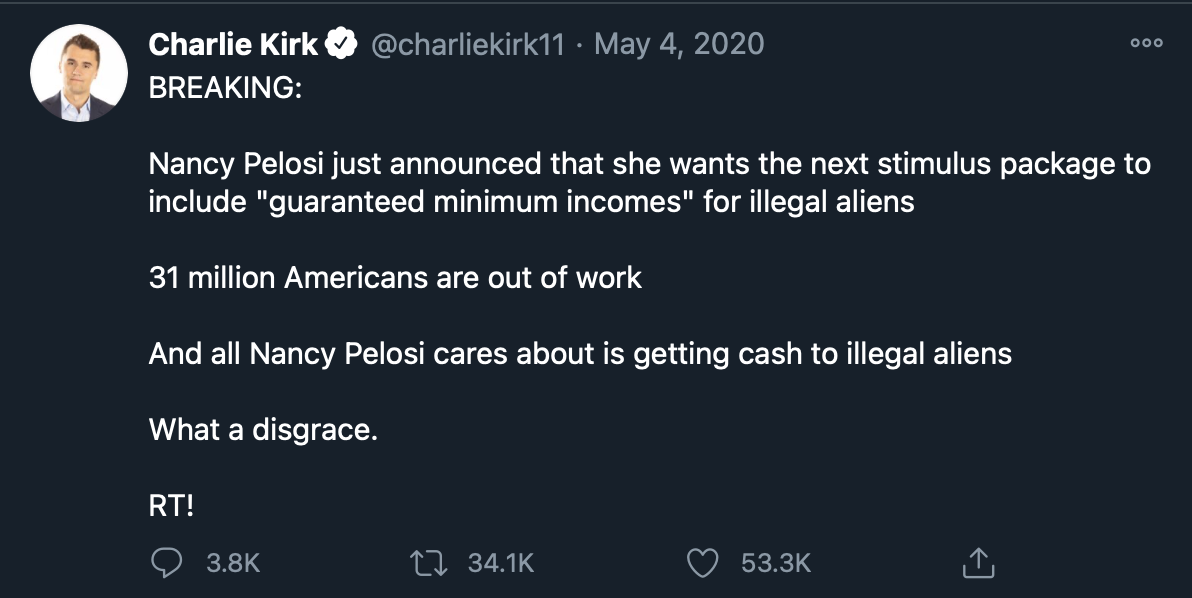
\includegraphics[width=11cm]{CharlieKirk Tweet.png}
    \caption{Charlie Kirk Tweet \cite{kirk2020tweet}}
    \label{fig:Charlie Kirk Tweet, May 4, 2020}
\end{figure} was rated "mostly false" by Snopes \cite{lee2020pelosi}: while Speaker Pelosi did say in an interview that she wanted to consider "guaranteed incomes" for Americans, including foreign workers without social security numbers \cite{pelosi2020maher}, she did not clearly define if "guaranteed income" meant the 2020 Paycheck Protection Plan (PPP) or something more akin to Universal Basic Income (UBI) as Kirk implies; she requested congress "consider it" and did not says she "wanted it"; both PPP and UBI would have directly affected \textit{all of} the 31 million Americans out of work rather than \textit{only} the undocumented immigrants as Kirk suggests. Therefore, since it is \textit{mostly} false but not \textit{completely} false, it would be unfair to say that $\tau_k = 0$ for this tweet; $ 0 < \tau_k < 0.5$ is more accurate. 


In another example, this tweet from Bernie Sanders is "mostly true" (fig. \ref{fig:Bernie Sanders Tweet, Oct 13, 2020}). 
 \begin{figure}[h]
    \centering
    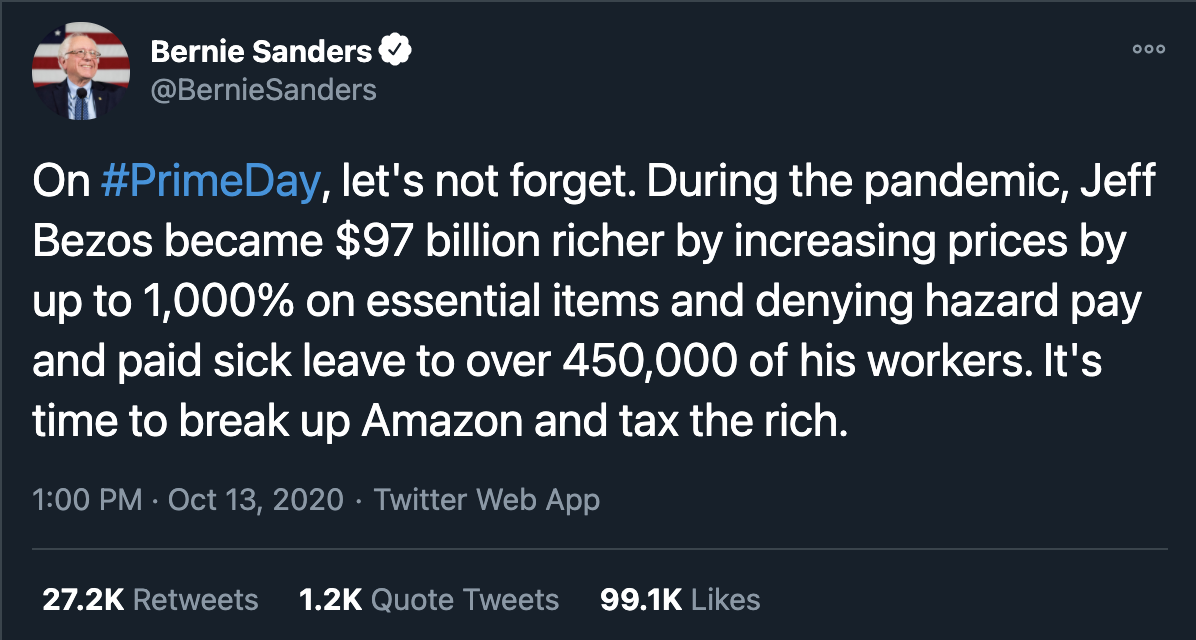
\includegraphics[width=11cm]{BernieTweet.png}
    \caption{Bernie Sanders Tweet \cite{sanders2020tweet}}
    \label{fig:Bernie Sanders Tweet, Oct 13, 2020}
\end{figure}
While it is true that Amazon's employees have been denied hazard or sick pay (or have struggled with the mostly automated Amazon HR) \cite{cnbc2020amazon,guardian2020amazon}, and Jeff Bezos's wealth increased by almost 80\% during 2020 due to Amazon's 40\% increase in sales year over year for Q2 (and the majority of his wealth is tied to Amazon shares) \cite{Stebbins2020bezos}, other articles discussing the increase in price on essential items point out that this was mostly Amazon \textbf{re-sellers} using the Amazon marketplace, not Amazon directly \cite{nicas2020sanitizer, kim2020price,gibson2020amazon}, Amazon banned over 6,000 of these price gougers \cite{bezos2020letter}, and that in cases where Amazon's price-generating AI had raised the price to an extreme level, it was returned to a reasonable level before Sen. Sanders wrote this tweet \cite{harman2020prime}. Therefore, it would not be reasonable to say that $\tau_s = 1$ for this tweet; it is $ 0.5 < \tau_s < 1$. 

Both Charlie Kirk's tweet and Senator Sanders's tweet fall under the purview of this thesis based on section \ref{Problem Statement}: they are both trying to influence a political discussion and use statements that are not entirely true to persuade susceptible readers. At the same time, they are not equivalent. Charlie Kirk's tweet featured a single true sentence and many surrounding falsehoods, while Senator Sanders's tweet had many true statements and one untrue (or at least misleading) statement. Much like how it was unreasonable to say $\tau_k = 0$ or $\tau_s = 1$, it is also unreasonable to say $\tau_k = \tau_s$. This nuance is meaningful and is not captured in the other literature. Therefore, an alternative solution to determining truth values must be used.

In \underline{Critique of Pure Reason}, Immanuel Kant proposed that statements should be broken into four groups: \textit{analytic a priori}, \textit{analytic a posteriori}, \textit{synthetic a priori}, and \textit{synthetic a posteriori} \cite{kant1908critique,frege1988collected,quine1951main}. \textit{Analytic} statements, per Kant, have the predicate contained in the subject, whereas \textit{synthetic} statements require a combination of understandings; \textit{a priori} statements are known without needing experience, whereas \textit{a posteriori} statements require experience to know if they are true \cite{wright1997companion}. 

A discussion on the four groups of statements, examples, and analysis are in \ref{truthvalue appendix}, but to summarize here, this thesis will only cover \textit{synthetic a posteriori} statements for which a truth value has not been determined. It will also cover statements that could be hyperbole, sarcasm, or irony (\ref{hyperbole}), as a random user may not immediately recognize that the content they are reading is sarcastic. It also does not differentiate between intentional and unintentional false statements. The question of intentionality is appropriate when determining punishment or if actions reach the level of fraud (and are therefore worthy of legal action), but it is not relevant to this thesis. A rapidly spreading false tweet about election fraud is equally destructive regardless of malicious intent.

It is important not to separate rumor from misinformation as Wu et al. or DiFonzo \& Bordia do since rumors can be just as destructive. In section \ref{Humanitarian Objection to Fake News Section}, examples were given regarding people who had committed suicide after being the victims of rumors \cite{starbird2014rumors,williamson2019alex}. The rumor that Antifa started the fires in Oregon hurt the firefighting efforts in the region  \cite{robinson2020oregon}. Baseless accusations of voter fraud led to five deaths in a riot at the capitol and the impeachment of a former US President \cite{fandos2021trump,Levenson2021capitol}.  Wu et al. and DiFonzo \& Bordia would have called all of these "rumors" up until they were officially debunked, yet this delineation did not stop them from having very deadly and serious consequences in the interim.

It also important to separate out hate speech, spam, and scientific misinformation from generalized misinformation (Table \ref{tab:misinformationexamples} in appendix \ref{truthvalueappendixsummary}). These are tasks that current machine learning is uniquely suited for, already have a great deal of available literature \cite{xu2019exploiting,wang2010detecting,ahmed2018detecting,al2019spam,oriola2020evaluating,gaydhani2018detecting,al2020lies,farrell2019evidence}, and which this thesis does not plan to improve upon. By narrowing this thesis's scope and using these other tools in an auxiliary fashion, this thesis can focus on curbing the viral spread of misinformation that is currently being insufficiently defended against. 



\section{Literature Review}
In all of the literature reviewed for this thesis on the topic fake news, there was very little if any time spent discussing the currently implemented solutions and their shortcomings. This thesis will try to rectify that and show why alternative solutions are needed in comparison to the status quo.

In Sec. \ref{sec: literature review}, there will be a brief analysis of other relevant literature and why they fall short of solving the problem.

\subsection{Currently Implemented Solutions}
\label{sec: currently implemented solutions}
This section will look at Facebook's current solution, as it is more robust than Twitter's. Twitter currently only allows for flagging of political misinformation that is directly related to a political event, census, or impersonation (fig \ref{img:TwitterPolitics}):
\begin{figure}[htp]
    \centering
    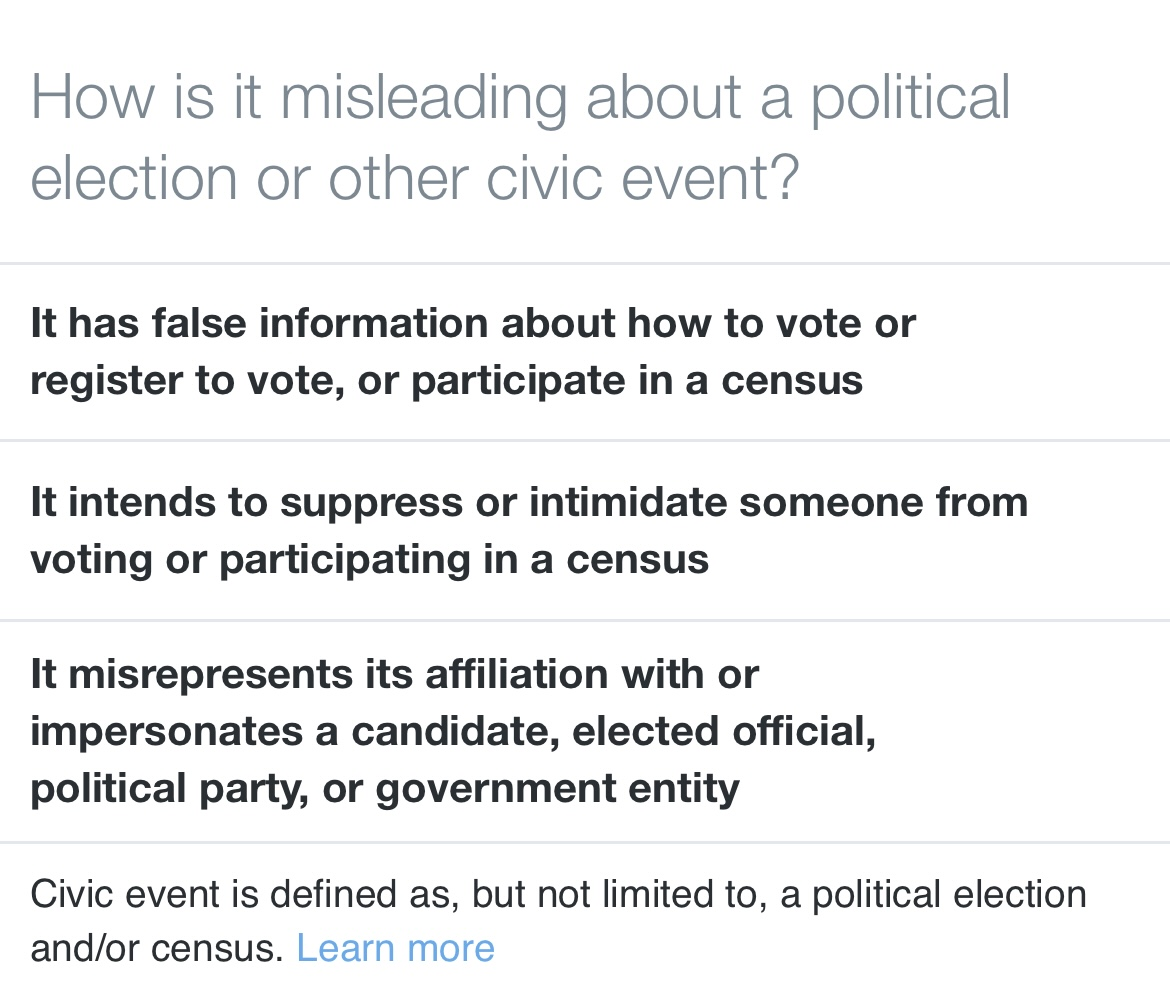
\includegraphics[width=6cm]{TwitterPolitics.jpg}
    \caption{Options for Flagging a Misleading Political Post on Twitter, Dec 2020}
    \label{img:TwitterPolitics}
\end{figure}

In his 2018 testimony to congress, Mark Zuckerberg stated that Facebook's processes with content reviewers had room for improvement, saying: \begin{quote}"... unfortunately, with the amount of content in our systems and the current systems that we have in place to review, we make a relatively small percent of mistakes in content review but that is too many, and this is an area where we need to improve..." \cite{energy2018facebook}\end{quote} and then pivoted to discussing the need for AI solutions, given the need for scalibility.

In his 2020 testimony to congress, Zuckerberg stated that they had tripled the security team to 35,000 employees, that they're funding new security technologies to prevent emerging fake threats such as "deep fakes", and that they have implemented resource centers for hot button topics like COVID-19 and the 2020 election \cite{zuckerberg2020}.


As of this thesis, Facebook currently has a preemptive solution and a two-step solution:
\renewcommand{\labelenumii}{\Roman{enumii}}
\begin{itemize}
\item The preemptive solution is to add a “context” button to all political posts, which a user can click on for more information \cite{smith2018designing}.
 \item If a post has been shared and is untrue, the following two-step solution is used:
 \begin{enumerate}
     \item It requires an outside individual to report the post. 
     \item After the post is reported, then it is  sent to 3rd-party fact checkers for verification. 
     \begin{itemize}
     \item Third party fact checkers must log in to the Facebook dashboard and then provide a link proving the story is false (they cannot simply mark a story as untrue) \cite{owen2016clamping}.
     \end{itemize}
 \end{enumerate}
 \end{itemize}
 
 In Facebook’s case, after they have determined a particular post is false, then the post is shown less frequently (80 percent less), other posts of the same link or image will also be shown less, it will be unable to be converted into an ad later, and someone re-sharing this post will be given a notification that the information is likely false \cite{owen2016clamping,facebook2020fact}.
 
 The punishment for routine offenders or for routine fake stories that point to a common domain is a loss of advertising rights and a loss of ability to monetize \cite{facebook2020fact}.
 
 %%%%%% 
 \subsection{Current Literature Alternative Solutions}
 \label{sec: literature review}
 The current proposed solutions from outside published journal articles generally fall into two groupings: tools that seek to recognize all misinformation and tools that seek to recognize particular subsets of misinformation (i.e. spam).

Language analysis is, clearly, a broad subject of analysis.  Castillo et al. use a decision tree based off emojis, symbols, etc. to attempt to predict misinformation \cite{castillo2011information}. Other textual analysis includes Qazvinian's analysis of speech tags \cite{qazvinian2011rumor}, Takahashi \& Igata's examination of "clue" words \cite{takahashi2012rumor}, Gupta et al.'s exploration of the usage of profanity \cite{gupta2014tweetcred}, Ghosh, Guo, and Muresan's investigation of word embeddings \cite{ghosh2015sarcastic}, Potomias, Siloas, and Stafylopatis's usage of a transformer \cite{potamias2020transformer}, Gaucho et al. review of tensor embeddings to detect content \cite{guacho2018semi}, Rubin et al. \cite{rubin2016fake} and Horne and Adali's \cite{horne2017just} usage of linguistic SVM classifications, Popat's investigation of how assertive verbs are in true vs. untrue content \cite{popat2017assessing}, and Riloff \cite{riloff2013sarcasm}, Pt{\'a}{\v{c}}ek et al. \cite{ptavcek2014sarcasm}, Buschmeier \cite{buschmeier2014impact}, and Barbieri's \cite{barbieri2014modelling} attempts to identify sarcasm.



For the tools that seek to recognize all misinformation, the most common solution is an RNN or an RNN/CNN combination. Ma et al. use a CNN to detect unique language patterns \cite{ma2018rumor} and Xu et al. use an RNN for the same purposes \cite{xu2019deep}, while Liu and Wu \cite{liu2018early}, Yang et al. \cite{yang2012automatic}, Wang et al. \cite{wang2018eann} Shu et al. \cite{shu2019role}, and Lee and Dernoncourt \cite{lee2016sequential}, Shu et al. \cite{shu2019beyond,shu2020leveraging} propose combination RNN/CNN solutions based off of text as well as user features (e.g. registration age) or visual clues to determine likely fake posts.  Other machine learning solutions also work off a combination of text and user information \cite{sun2013detecting,kwon2017rumor,ma2015detect,ma2016detecting,zhao2015enquiring}. VanDam uses a combination of a supervised and supervised neural network to detect hashtag and account hijacking \cite{vandam2019learning}. Chen proposes an improvement to the RNN solutions by using an attention based RNN \cite{chen2018call}. Khoo et al. also use an attention based transformer and include a hierarchical token and post level model as well \cite{khoo2020interpretable}. Zhou's SAFE model is CNN only, but it attempts to cover the same ground in a similar fashion \cite{zhou2020mathsf}.

In terms of graph analysis, Wu, Yang, and Zhu \cite{wu2015false} use a graph-kernel SVM to classify misinformation as does Ma at al. \cite{ma2017detect}. Jin et al. \cite{jin2013epidemiological} and Wu et al. \cite{wu2016mining} both identify that this problem is naturally suited to epidemiological spread. Ren et al. use a Graph Neural Network (GNN) to classify news sharing nodes \cite{ren2020adversarial} -- a similar goal to other works that focus on the user sharing the content. Hamid et al. use a GNN with a Bag of Words and BERT model \cite{hamid2020fake}, Han et al. use a GNN with continual learning \cite{han2020graph}, Rath, Morales, and Srivastava use an attention based GNN \cite{rath2021scarlet}, while Benimara et al. use a combination of semi-supervised learning and a GNN to solve the problem \cite{benamira2019semi}.  Gupta et al. use a graph optimization approach \cite{gupta2012evaluating}, while others use a propagation model which tracks the cascade of content \cite{jin2016news,jin2014news,zhou2018fake,kashima2003marginalized}. Huang et al. use a combination of a GNN and a propagation model \cite{huang2019deep}. Ciampaglia et al. \cite{ciampaglia2015computational} and Shi and Weninger \cite{shi2016discriminative} use knowledge graphs and subject-predicate-object triples. Mishra et al. have used GNN's for abuse detection \cite{mishra2019abusive}, Li and Goldwasser \cite{li2019encoding} and del Tredici et al. \cite{del2019you} for political partisanship detection. 


Han et al. \cite{han2020graph}, Nguyen et al. \cite{nguyen2020fang}, and Chandra et al. \cite{chandra2020graph} have applied GNNs recently to the topic of fake news detection. 

 Shin et al. observe that there is a temporal relationship between rumors and truth and that misinformation can be traced to highly partisan sources \cite{shin2018diffusion}.
 
 
 van der Liden, Roozenbeek, and Compton argue that "pre-bunking" or sharing truthful information before misinformation can spread can serve as a form of viral inoculation against misinformation \cite{van2020inoculating}.
 
 \subsection{Issues with Solutions Discussion in Section \ref{sec: currently implemented solutions} and \ref{sec: literature review}}
 \subsubsection{Issues with Preemptive Solution}
 Facebook's proposed "context" button (a way for users to get extra context around an article) is ineffective for several reasons. 
 
 First, it assumes that people will actively search for context when viewing a link. People are unlikely to feel the need to do further research if they agree with or believe the headline as presented \cite{nyhan2010corrections}. This problem is augmented by the fact that headlines are often misleading and written to draw the strongest possible emotional response \cite{chesney2017incongruent,ecker2014effects,bell1984good,molek2013towards,kilgo2018new,vettehen2008explaining}. An example from the \textit{Express} newspaper in the UK (from Ecker, et al.):
 \begin{itemize}
 \item Headline: Air pollution now leading cause of lung cancer
\item Evidence within article: “We now know that outdoor air pollution is not only a major risk to health in general, but also a leading \textbf{environmental} cause of cancer deaths.” Dr. Kurt Straif, of IARC [emphasis added]
 \end{itemize}
 
 Or from the \textit{Independent}'s Facebook page \cite{chesney2017incongruent}:
 \begin{itemize}
\item Social media post copy: Enjoy it while you
can
\item Social media headline \footnotetext[1]{https://www.facebook.com/TheIndependentOn-line/posts/10154972799736636}\footnotemark[1]: Scientists have predicted the end of sex
\item Article headline\footnotemark[2]\footnotetext[2]{Will Worley (2016): http://www.independent.co.uk/news/science/sex-unnecessary-designer-babies-stanfordprofessor-says-a6957636.html}: Sex will be made unnecessary by ‘designer babies’, professor says
\item Evidence within article: Professor Henry Greely believes that in as little as 20 years, most children will be conceived in a laboratory, rather than through sexual intercourse.
 \end{itemize}
 
 While there have been attempts to track down misleading headlines, they have primarily centered around \textit{click-bait} or tabloid headlines \cite{chen2015misleading,chakraborty2016stop} that require the user to click to find out the information, i.e. "Here’s What Happens When You Put A Few Little Kids In A Room With 2 Dolls In 2 Different Colors" \cite{chen2015misleading}. While this will help with some problems, both the \textit{Express} and \textit{The Independent} articles would not be caught by the proposed algorithms. 
 
 
Given that only 59\% of all shared URLs are ever clicked on Twitter \cite{gabielkov2016social} and there is clear evidence of misleading headlines, Twitter added in a feature that prompts users to read articles rather than just headlines before sharing the article \cite{reuters2020article}. Unsurprisingly, the backlash was immediate (fig: \ref{fig:House Judiciary GOP Tweet}):
 \begin{figure}[htp]
    \centering
    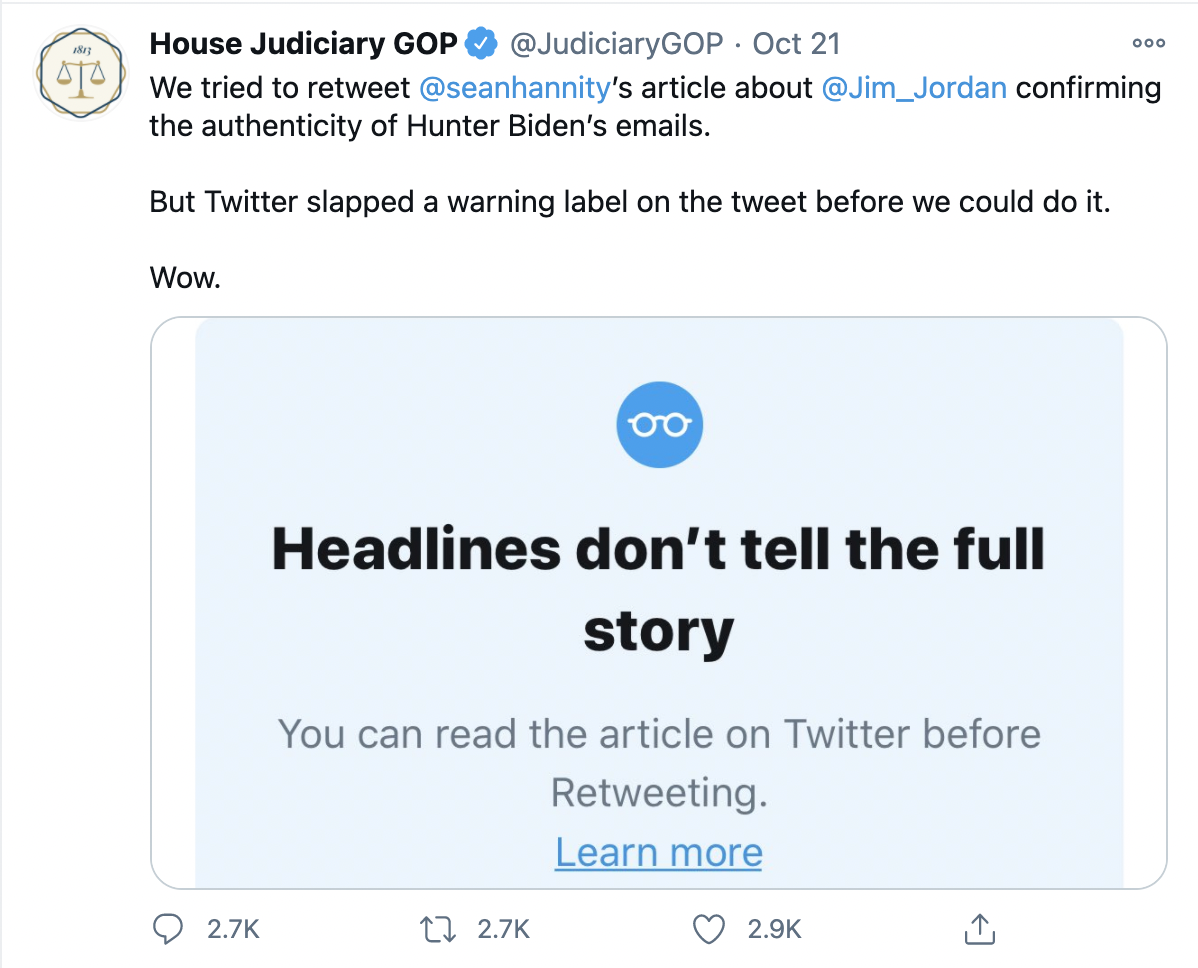
\includegraphics[width=8cm]{JudiciaryTweet.png}
    \caption{House Judiciary GOP Tweet}
    \label{fig:House Judiciary GOP Tweet}
\end{figure}

As will be discussed in section \ref{sec: echo chambers}, this fits the problem of \textit{echo chambers} wherein the primary question is not "is this correct" but "does it align with the views of my network?" 

To summarize, the proposed preemptive solution of a "context" button is ineffective because:
\begin{itemize}
\item 41\% of the time, someone will retweet an article without having read more than the headline. \cite{gabielkov2016social}
\item Headlines are written to be intentionally misleading, or at least to generate a strong emotional response from the reader.\cite{chesney2017incongruent}
\item Readers are unlikely to fact-check, question, or feel compelled to do outside research on an article if the have a strong emotional response to it.\cite{nyhan2010corrections}
\item Blanket warnings without explanation are likely to generate backlash \cite{reuters2020article}
 
 \end{itemize}

\subsubsection{Issues With the Two-Step Solution: Echo Chambers}
\label{sec: echo chambers}
 The key first step for the two-step solution is that an individual must report the post as false. This requires a level of self policing that it is unlikely given the prevalence of \textit{echo chambers}. 
 
Because social media seeks to connect like minded individuals, it has a tendency to generate \textit{echo chambers}, or closed networks with high repetition of content and low diversity of thought \cite{adibi2005proceedings, bastian2009international, pariser2011filter,bozdag2015breaking}. While not every closed homogeneous network is inherently bad -- they can operate as self-help groups \cite{kast2012under} or can encourage positive behavior like reducing prejudice \cite{paluck2011peer} -- there is a clear and well documented history that people are influenced by others in their network \cite{cialdini2004social,bollinger2012peer, bond201261,gerber2008social,gerber2009descriptive,meer2011brother,paluck2012salience,del2016spreading,bessi2015viral,friedkin1984structural,marsden1993network} and this can be destructive in the context of misinformation. For this paper's purposes, partisanship $\rho$, is defined as being on a scale of 0 to 1 with 0 being extremely left-wing and 1 being extremely right-wing (a normalized version of most one-dimensional scales of the topic). Therefore, for all users $u$ in the set of users $U$:
\begin{equation}
\label{basepartisanship}
    \forall \ u \in U \ \exists \ \rho \in \mathbb{R} \ | \ 0 \leq \rho \leq 1
\end{equation}
From here, $\rho_k$, the partisan leaning of some unique user $u_k$ is directly proportional to the average partisan leaning of the \textit{echo chamber} network $n_n$ (here and elsewhere, a network, $n$, is defined as the total set of "neighbors" or other nodes that the user is connected to either by following or being followed by) and can be described as follows:
 \begin{equation}
    \label{ech chamber}
        \langle \rho_n \rangle = \frac{1}{|n_n|}\sum_{i=1}^{|n_n|}{\rho_i}, (u_i \in n_n, n_n \in N)
 \end{equation}
 \begin{equation}
    \label{leaningproportionaltonetwork}
        \rho_k \sim \langle \rho_n \rangle
 \end{equation}
 
 For validation of this, in Asch's classic experiment, he found that individuals will conform to the opinions of the rest of the group, even if it runs contrary to their personal convictions \cite{asch1956studies}. For a more recent political example, in Bullock's experiments he found that participants would change their opinions on a particular topic if they were told that the party they identify with held an opposing view, even if it was counter-intuitive, such as a Republican being told that the Republican party was against a conservative initiative \cite{bullock2007experiments}. Other research provides similar results: Republicans and Democrats are likely to accept a statement as being true and not feel the need to research personally if it comes from a preferred politician \cite{housholder2014facebook}. Even if a preferred politician's statements are disproved, there is no shift in voting intentions, party identification, or overall perceived credibility of that politician \cite{swire2017processing}. 
 
 From a network theory perspective, equations \ref{ech chamber} and \ref{leaningproportionaltonetwork} combine to a slightly simplified version of the Hopfield attractor network \cite{hopfield1982neural,hopfield1985neural,nowak1998toward,kitts1999structural}, as set forth by Macy et al.\cite{macy2003polarization}. The Macy et al. equation illustrates social pressure towards a binary (accept/reject) of a particular position based upon the number of members of the network, the position, and a weight, $w$, which represents the dyadic tie between a node's "friends" and "enemies" (here \textit{i} is a "friend" and \textit{j} is an "enemy"):
\begin{equation}
 \label{macy equation}
 P_{is}=\frac{\sum^{N}_{j=1}w_{ij}s_{j}}{N-1},j\neq i
\end{equation}
Clearly, combining equations \ref{ech chamber} and \ref{leaningproportionaltonetwork} and removing the concept of "friends" and "enemies", is the same as \ref{macy equation}. It merely substitutes the term "network pressure" with "network average partisanship".
 
 
This provides a perfect opening for malicious actors, as they are primarily focused on sharing and inflaming hyper-partisan and extreme views \cite{shin2018diffusion,bastos2019brexit,hegelich2016social,mueller2019mueller}, such that the partisanship of a malicious actor, \textit{m}, from the set of malicious actors, \textit{M}, will be extreme: 
\begin{equation}
\label{trollpartisanship}
\forall \ m \in M, \exists \ \rho \in \{0,1\}.
\end{equation}

Mirroring viral spread seen in other scale-free network analyses \cite{pastor2001epidemic,cohen2003efficient}, this problem quickly escalates: as the number of malicious actors in the network, $|M| \in n$, increases, the group partisanship will shift towards the \{0,1\} binary, as can be seen by combining equations \ref{trollpartisanship} and \ref{ech chamber}: 
\begin{equation}
\langle \rho \rangle \rightarrow \rho_m \in \{0,1\}
\end{equation} 
And given Bullock's experiments and equation \ref{leaningproportionaltonetwork}:
\begin{equation}
\label{peopletoextremes}
    \forall u \in n: \rho \sim \langle \rho_n \rangle: \rho \rightarrow \rho_m
\end{equation}
Equation \ref{peopletoextremes} correlates perfectly with the social experiments by Asch and Bullock mentioned previously, and more recent research has confirmed these findings \cite{colliander2019fake,edelson2011following}. Even when the groups were anonymous users on the internet, users were still be motivated by a desire to conform to the group's opinions and would, if necessary, relinquish their own previous beliefs in order to fit in \cite{williams2000cyberostracism,zhu2012switch,tsikerdekis2013effects,breitsohl2015groupthink,winter2015they,hamilton2017s}. 

The closer $\langle \rho \rangle$ gets to 0 or 1, the more closed the network becomes, and the more resistant to fact-checking or corrective information coming from outside of their network \cite{garrett2013undermining,lord1979biased,edwards1996disconfirmation,redlawsk2002hot, taber2006motivated}. This explains both why even the release of President Obama's long form birth certificate only briefly subdued the conspiracy that he was not born in the United States \cite{nyhan2012new} and why the Pizzagate conspiracy discussed in Sec. \ref{introduction} lived even after it had been disproved months earlier -- so long as the corrective information came from outside of the echo-chamber, it was fundamentally dismissed.


\subsubsection{Partisanship} 
\label{Partisanship Section}
There is substantial research that Americans who identify as right-wing have historically been more susceptible than other subsets of the American population to fake news \cite{guess2019less,benkler2018network,grinberg2019fake,allcott2017social,badawy2018analyzing}, but more thorough analysis suggests that this pattern may not hold up moving forward.

First, there may be an over representation in terms of conservative vs. left misinformation in the analyzed data sets. In the Russian troll data set provided by Twitter, there were twice as many right leaning trolls as left leaning trolls \cite{freelon2020black,badawy2018analyzing,benkler2018network}. The Russian "troll farm" known as the Internet Research Agency (IRA) created a wide range of political Facebook groups,\begin{quote}
    ... [which] included purported conservative groups (with names such as “Being Patriotic,” “Stop All Immigrants,” “Secured Borders,” and “Tea Party News”), purported Black social justice groups (“Black Matters,” “Blacktivist,” and “Don’t Shoot Us”), LGBTQ groups (“LGBT United”), and religious groups (“United Muslims of America”)\cite{mueller2019mueller};
\end{quote} however, the Mueller report goes on to note that "throughout 2016, IRA accounts published an increasing number of materials supporting the Trump Campaign and opposing the Clinton Campaign." It is likely that this is a positive feedback loop. Since conservatives were more likely to consume fake news, there were more IRA trolls creating fake content for them, which  in turn these conservative users would be more likely to share \cite{bakir2018fake,bodo2019interested,silverman2016analysis,pariser2011filter}. 


Second, a better predictor of willingness to share misinformation is general distrust in the media rather than political leaning \cite{hopp2020people,shin2017partisan,kahan2012ideology,lewandowsky2016motivated,swire2017processing,mourao2019fake}. This is further born out by the IRA heavily targeting two groups they determined were unlikely to trust the main stream media: far right-wing Americans and Black Americans \cite{diresta2019tactics,howard2019ira,boatwright2018troll,jamieson2020cyberwar,mueller2019mueller,freelon2020black}. In fact, the IRA spent a disproportionately high amount in micro-targeting Black Americans and generated a high return on their investment (the average misinformation post targeted at a Black American was 2.5 times more likely to receive an engagement, such as a like or retweet, from a real user than a misinformation post targeted at a general conservative American) \cite{howard2019ira,freelon2020black}.

Third, many sharers of misinformation are more focused on empathy with a particular group \cite{winter2015they,rheault2016measuring,dale2017nlp} or engaging in signaling theory with a group \cite{connelly2011signaling,lampe2007familiar,spence2002signaling} rather than objective truth. Dominic Cummings callously stated while creating inaccurate content for the Leave campaign for Brexit that "accuracy is for snake-oil pussies" \cite{crace2016accuracy}, yet his point is widespread and in line with the analysis of \textit{echo chambers} in section \ref{sec: echo chambers}: in hyper-partisan situations, strongly held opinions that are counter to widely accepted narratives are seen primarily as signals of commonality \cite{yla2018populist,noppari2019user,lazer2018science,yla2019politicization,wasilewski2019us,freelon2020russian}. 


Fourth, there is no difference in propensity to share non-partisan misinformation, such as the dangers of living near power lines, the side-effects of MMR vaccines, or the safety of nuclear power reactors between people of various beliefs \cite{kahan2015climate,hara2016co,kahan2012ideology,lewandowsky2016motivated,barbera2015tweeting}.

Finally, most of the studies referenced previously in this section used data from 2015/2016 and before for their analysis. Since 2015, there has been a well documented global rise in populism on the left end of the spectrum to match the rise on the right that had previously existed and was documented earlier. For example, there was a 33x increase in membership in far-left organizations such as the Democratic Socialists of America between 2015 and 2020 \cite{godfrey2020thousands}, left-leaning populist groups in France saw outsized social media volume in the 2017 elections \cite{donadio2017french}, and the U.K's Labour party took a shift to the populist left under the leadership of Jeremy Corbyn starting in 2015 \cite{wainwright2018remarkable,hobson_fielding_2019}. 

This polarized shift can be statistically seen in the United States Congress by comparing the voting patterns of the 115th (Jan 2017 - Jan 2019) (fig. \ref{fig:115th House}) and 116th (Jan 2019 - Jan 2020) (fig. \ref{fig:116th House}) House of Representatives \cite{fivethirtyeight2018tracking}. In both of these illustrations, Democrats are blue, Republicans are red, Independents are orange, and the scale for each Representative is the same $0\leq \rho \leq 1$ scale seen in equation \ref{basepartisanship}. Here, a representative who always voted in line with President Trump's position (if he gave one on a particular bill) has $\rho = 1$, and someone who never voted in line with President Trump has $\rho = 0$:

 \begin{figure}[h]
\minipage{0.5\textwidth}
  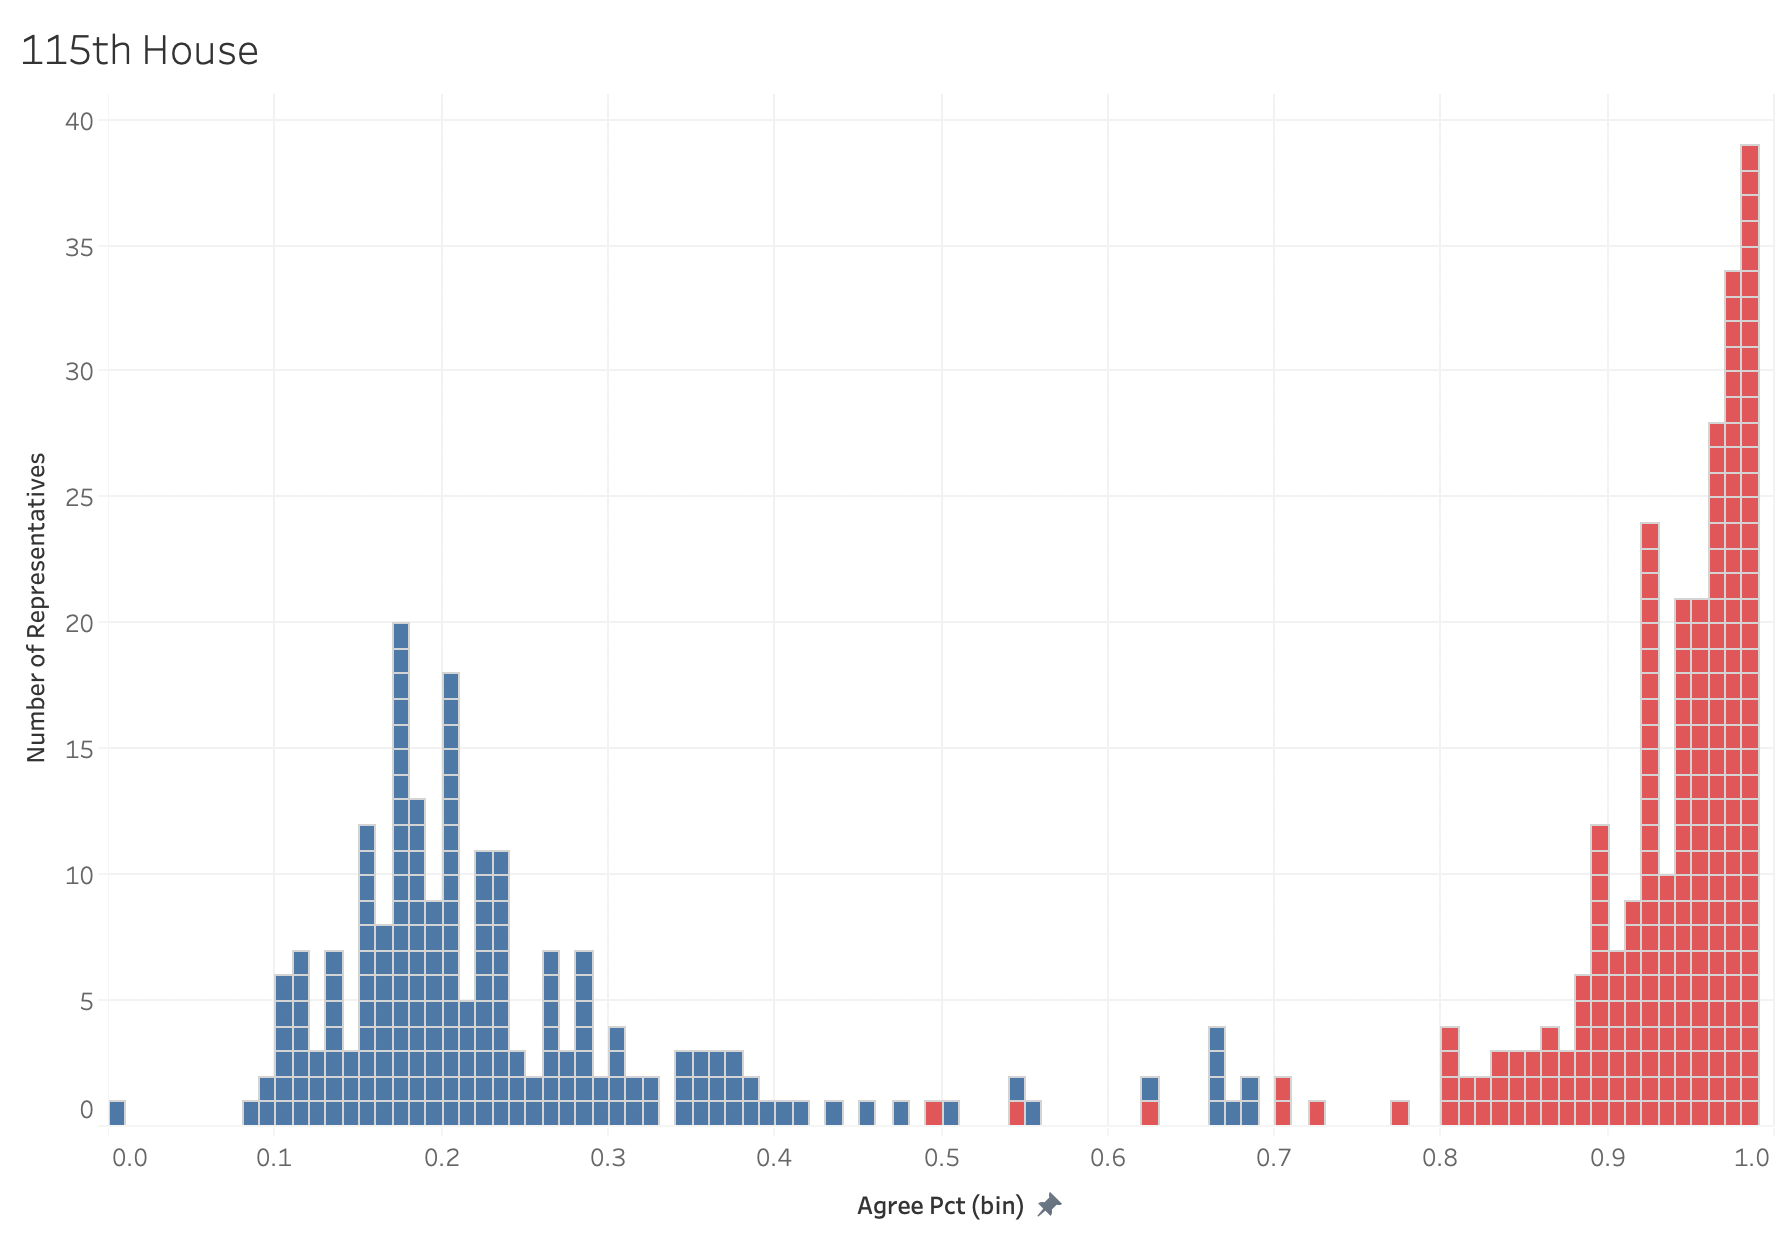
\includegraphics[width=\linewidth]{115th House.png}
  \caption{115th House of Representatives}\label{fig:115th House}
\endminipage\hfill
\minipage{0.5\textwidth}
  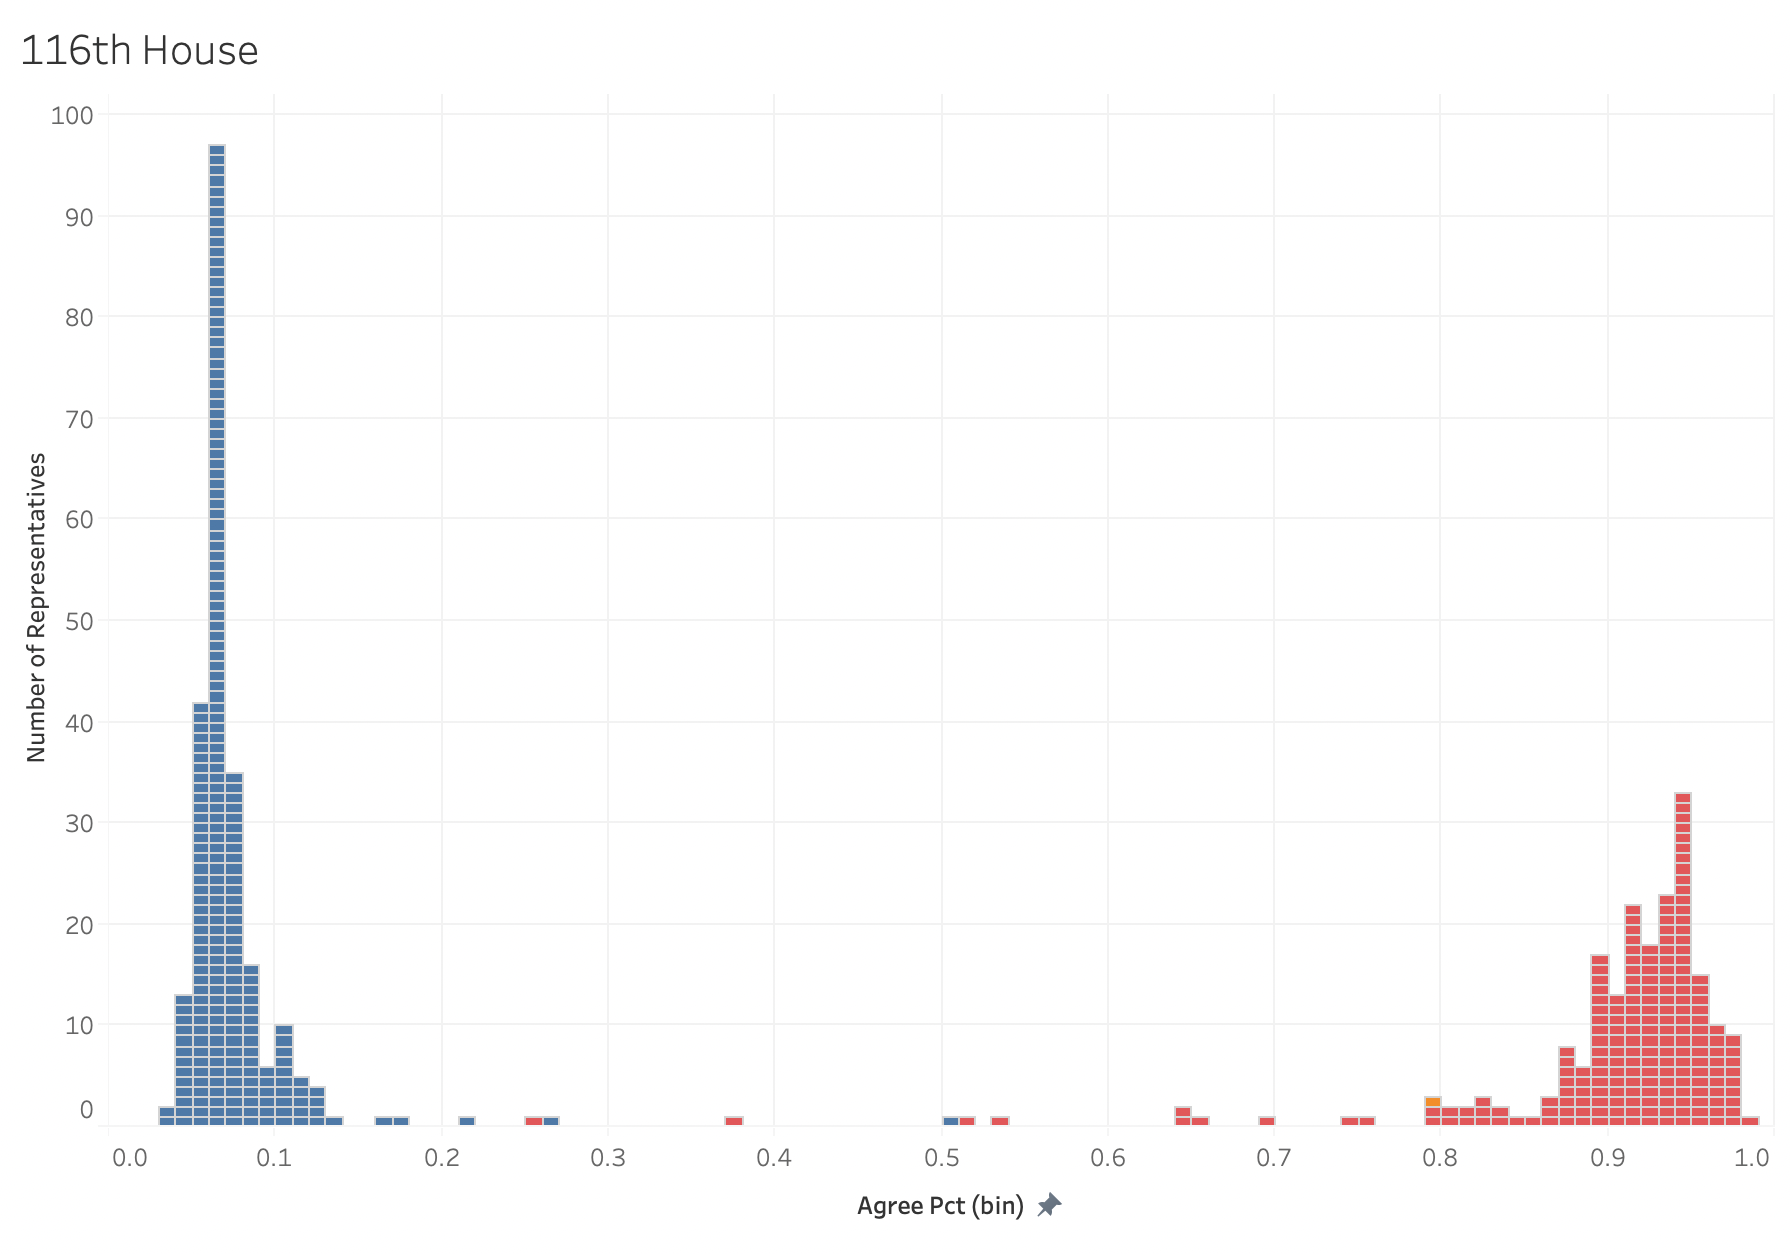
\includegraphics[width=\linewidth]{116th House.png}
  \caption{116th House of Representatives}\label{fig:116th House}
\endminipage\hfill
\end{figure}
 
 In the 115th congress, Republican members had an average $\langle \rho_r \rangle = 0.93$ and Democratic members had an average $\langle \rho_d \rangle = 0.24$. In the 116th congress, Republican members had an average $\langle \rho_r \rangle = 0.91$, Democratic members had an average $\langle \rho_d \rangle = 0.08$, and Independent members had an average $\langle \rho_i \rangle = 0.79$. While the Democratic party did pick up +40 seats in the 2018 midterms, simply adding or subtracting members does not imply a shift in partisanship as the Republican partisanship barely changed between the 115th and 116th Congress. For the state of Pennsylvania, which very narrowly broke for President Trump in 2016, the Democratic members had a $\langle \rho \rangle = 0.39$ in the 115th Congress and a $\langle \rho \rangle= 0.07$ in the 116th.
 
 For comparison, the US Senate is somewhat more stable, possibly because Senators are only up for election every 6 years instead of every 2, so turnover is less frequent. In the 115th congress, Republican senators had an average $\langle \rho_r \rangle = 0.91$, Democratic senators had an average $\langle \rho_d \rangle = 0.30$, and Independent senators had an average $\langle \rho_i \rangle = 0.30$. In the 116th congress, Republican senators had an average $\langle \rho_r \rangle = 0.83$, Democratic senators had an average $\langle \rho_d \rangle = 0.19$, and Independent senators had an average $\langle \rho_i \rangle = 0.22$.
 
 As illustrated before, a shift in the average partisanship of the network towards the \{0,1\} binary strongly correlates to populism and a susceptibility to misinformation \cite{hopp2020people,kahan2012ideology,mourao2019fake,shin2017partisan,swire2017processing,vargo2018agenda}. This can already been seen anecdotally, as there has been an uptick in left-leaning misinformation (or hyper-partisan opinions counter to the general accepted facts, per point two of this section)  since 2018, including information around a confrontation between MAGA-hat wearing teenagers, Black Israelites, and a Native American elder at the Lincoln Memorial in 2019 \cite{sacks2019maga,healy2019believing,pond2020complexity}, and the death of Breonna Taylor in 2020 \cite{duvall2020fact,kim2020fact}. 

 \subsubsection{Third Party Fact Checkers}
  \label{Third Party Fact Checkers Sections}
 The usage of third party fact checkers has two fundamental issues.
 
 First, there is a large volume of research over decades that ideologues on either side of the political spectrum will view the exact same content as being biased against them \cite{arpan2003experimental,baum2008eye,christen2002hostile,gunther2001predicting,gunther2004mapping,baum2004issue,gussin2004eye,lee2005liberal,vallone1985hostile}. This extends to fact-checking, as groups on both the left and the right post about claims of censorship when their content is removed or their reach is reduced \cite{Dreyfuss2020Now,Post2020Facebook,Millhiser2018Facebook}. 
 
 As Shin and Thorson note, however, closed networks are eager to fact check members who are not of their group. In 2018, Think Progress (a liberal Facebook fact-checker and an online journal) posted an article on the Brett Kavanaugh Supreme Court confirmation hearing that was flagged as false by The Weekly Standard (a conservative Facebook fact checker) \cite{lybrand2018kavanaugh}. Think Progress had stated that then-Judge Kavanaugh had said during his hearing that he would kill Roe v. Wade (Fig. \ref{fig:Think Progress Headline})\cite{millhiser2018brett},
  \begin{figure}[h]
    \centering
    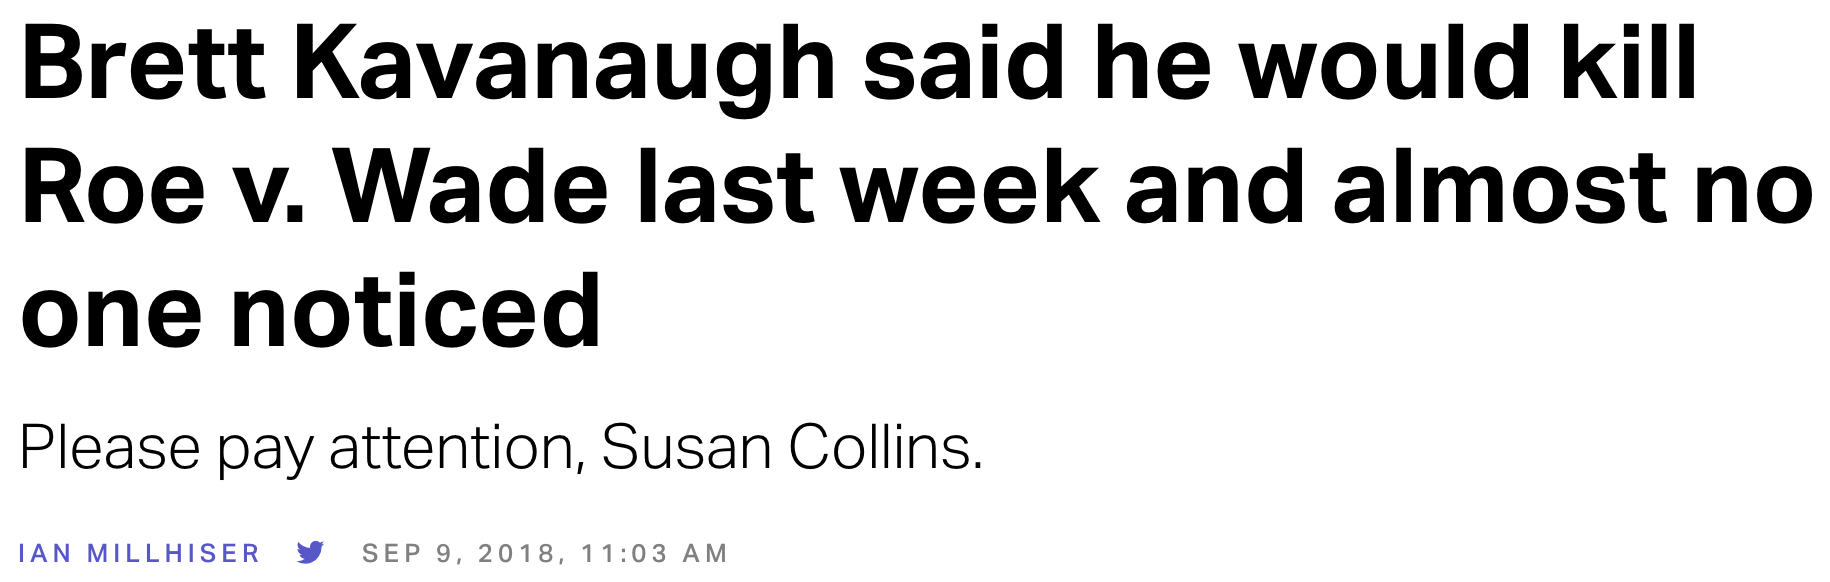
\includegraphics[width=11cm]{ThinkProgress Headline.png}
    \caption{Think Progress Headline \cite{millhiser2018brett}}
    \label{fig:Think Progress Headline}
\end{figure} a claim that was deemed false by the Weekly Standard and by FactCheck.org, a non-partisan fact-checking organization \cite{gore2018kavanaugh}. The Weekly Standard offered to remove its flag if Think Progress replaced the word "said" in the headline, as Judge Kavanaugh had not explicitly said that he would overturn Roe v. Wade (Fig. \ref{fig:Rachael Larimore Tweet, Sep 11, 2018}).
 
 \begin{figure}[h]
    \centering
    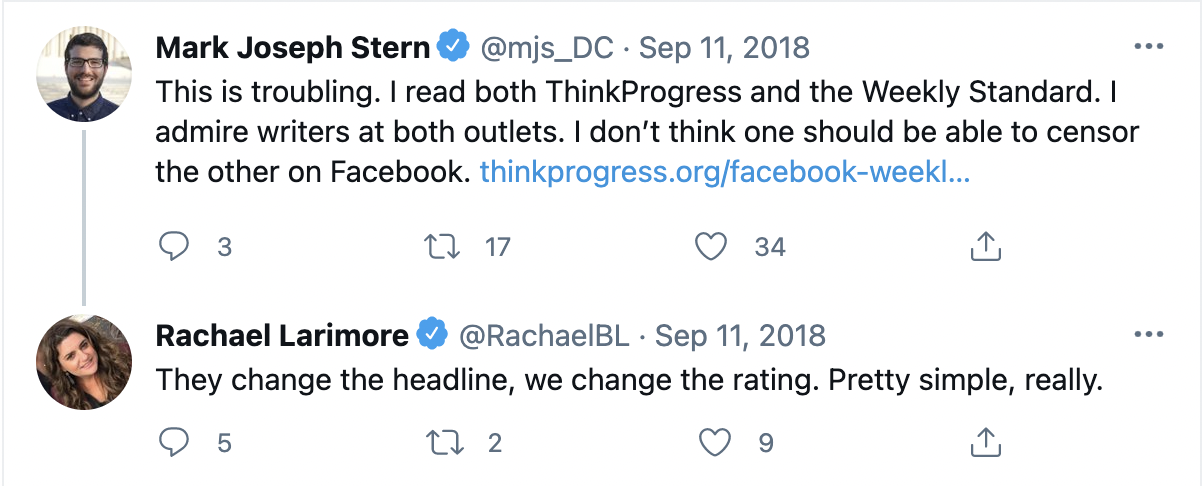
\includegraphics[width=11cm]{Larimore Tweet.png}
    \caption{Rachael Larimore Tweet \cite{larimore2018tweet}}
    \label{fig:Rachael Larimore Tweet, Sep 11, 2018}
\end{figure} 
Think Progress argued that secondary and tertiary definitions of "said" made their headline correct, and instead accused Facebook of bias and censorship \cite{legum2018tweet}. They also demanded that the Weekly Standard be removed from the list of fact-checkers \cite{Millhiser2018Facebook}, ignoring that other fact-checking organizations also rated Think Progress's assessment as false \cite{gore2018kavanaugh,tobias2018kavanaugh}.
Shortly after, several other liberal journalists made the same argument of censorship with none touching on whether or not the word "said" was truthful \cite{froomkin2018tweet,grim2018tweet,beutler2018tweet}. It is also worth noting that Think Progress used this identical argument (that saying someone "said" something if they did not directly say it was false and grounds for content to be removed) when fact-checking conservative articles on Barack Obama \cite{legum2008context}, Joe Biden \cite{volsky2016biden}, James Comey \cite{israel2018rnc}, James Clapper \cite{lerner2015cruz}, and others. 
 
 This example matches the previous analysis of strongly held partisan views being "truer" than objective truth. It also aligns with other research that shows that closed groups are more than eager to fact-check individuals who do not belong to their group, such as Republicans fact checking Democrats and vice-versa \cite{shin2017partisan,iyengar2015fear}, and that they are unable or unwilling to recognize potential mischaracterizations of opposing viewpoints \cite{pennycook2019lazy,vargo2018agenda}. 
 
A better solution, clearly, would be only to use high quality non-partisan fact checkers, as they would be able to rise above the echo chamber issues. However, these well-regarded apolitical fact checkers, such as Snopes and the Associated Press, have either left their fact checking partnership with Facebook or stopped actively working. They argue that Facebook's process is manual, time consuming, ineffective, and does not provide adequate compensation for the time required to do the job thoroughly \cite{green2019message,coldeway2019update}. An ideal solution, then, most be one which limits the amount of time-consuming manual work, hence Zuckerberg's initial comments about AI being the key to solving this problem.

\subsubsection{Issues with Punishment}
\label{Issues with Punishment Section}
By this point, it should be clear that the punishments imposed by Facebook are not effective, as they only seek to limit ad revenue and the ability to monetize. This implies a financial incentive for purveyors of incorrect information where, as has been shown, much of this is ideologically driven \cite{allcott2017social}. While these may be effective deterrents for the \textit{click-bait} or tabloid style headlines discussed earlier  \cite{chen2015misleading}, less than 0.1\% of traffic to fake news websites during the 2016 election came from paid media/advertising \cite{albright2016election2016}. 

The other key punishment that Facebook implements is on the actual post level. Posts deemed false are shown 80\% less frequently, and other posts showing the same link or image will also be shown less frequently. While this sounds promising, there is a fundamental flaw that can be exposed by examining Facebook's most recent papers on computer vision. Facebook's AI is a Convolutional Neural Network (CNN) \cite{carion2020end}, which is very good for detecting something in common across several images, such as a person's face \cite{kalinovskii2015compact}, but is easily fooled by changing parts of the image, such as adjusting font and colors, cropping, adding filters, etc \cite{sumbaly2020using}.

For example, this shutterstock image of Donald Trump (fig. \ref{fig:Trump Shutterstock Image}): 
 \begin{figure}[htp]
    \centering
    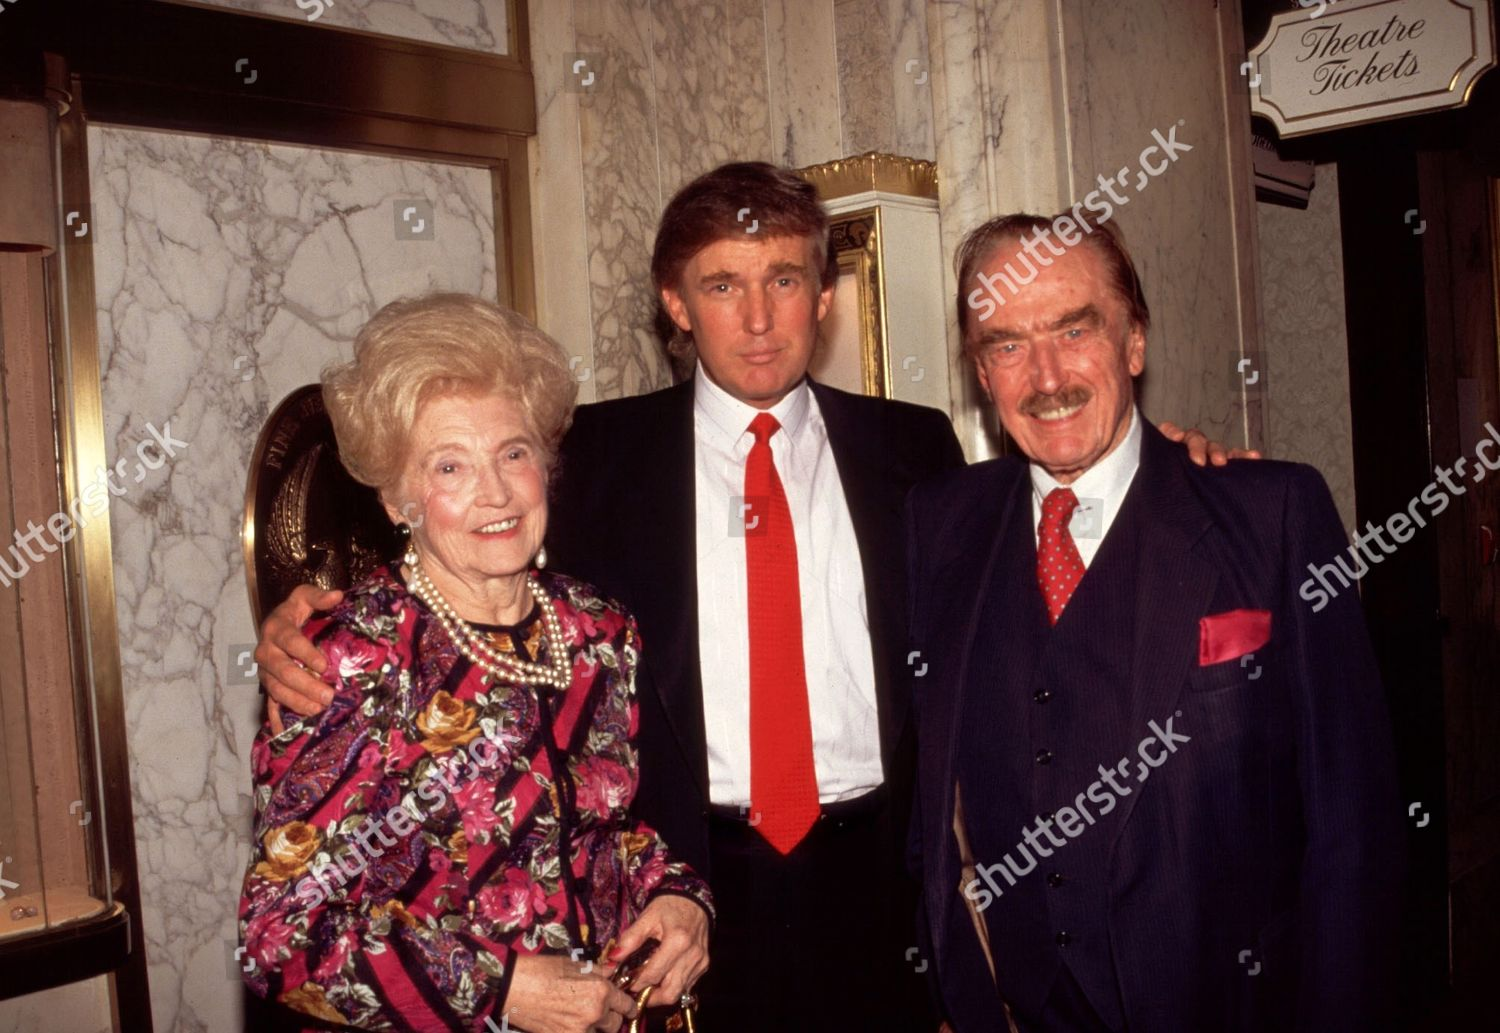
\includegraphics[width=8cm]{trumpkkk0.jpg}
    \caption{Trump Shutterstock Image}
    \label{fig:Trump Shutterstock Image}
\end{figure}

was photoshopped to make it appear as though his parents were wearing KKK robes. Reuters provided three different examples of the image that were widely shared on social media \cite{reuters2020trump} (Figures \ref{fig:TrumpKKK1}, \ref{fig:TrumpKKK2}, \ref{fig:TrumpKKK3}).

 \begin{figure}[h]
\minipage{0.32\textwidth}
  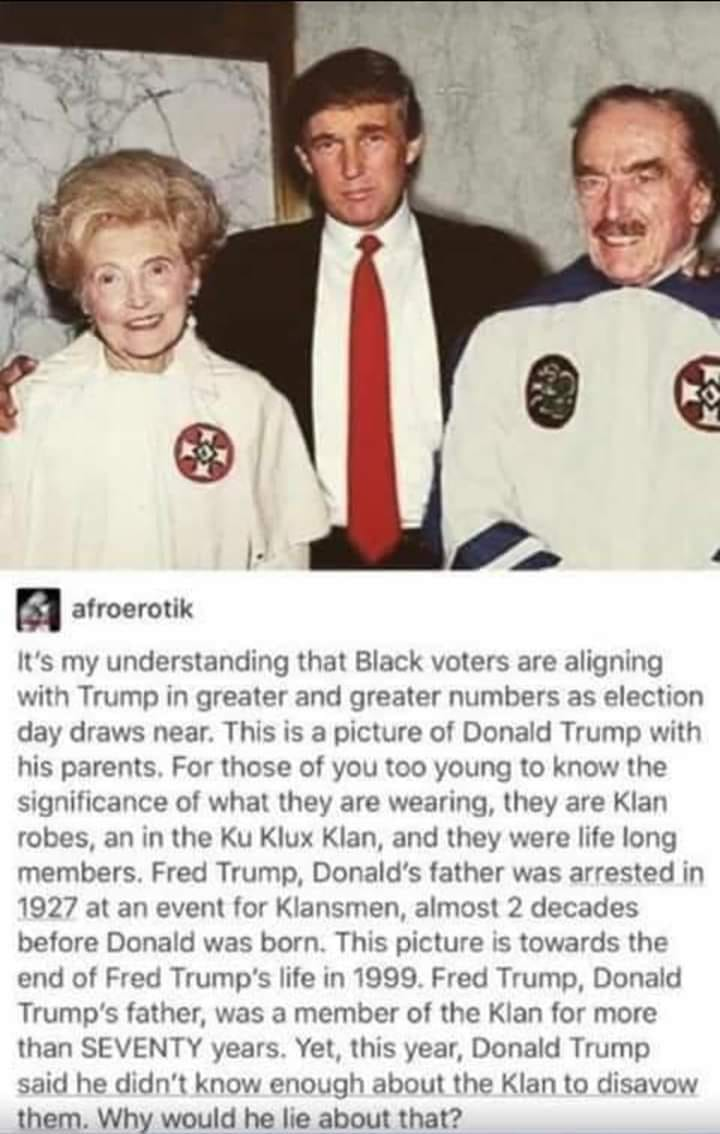
\includegraphics[width=\linewidth]{trumpkkk1.jpg}
  \caption{Version 1 of Edited Trump Image}\label{fig:TrumpKKK1}
\endminipage\hfill
\minipage{0.32\textwidth}
  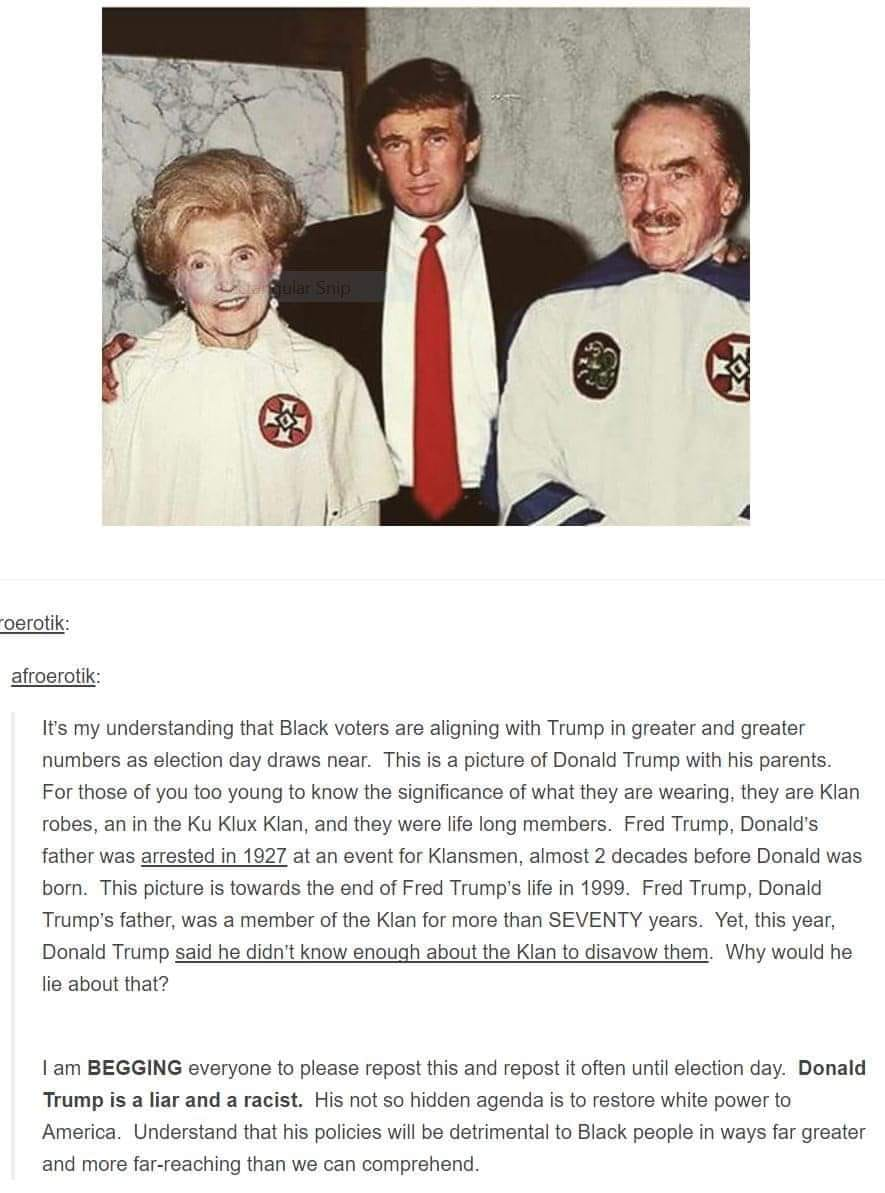
\includegraphics[width=\linewidth]{trumpkkk2.jpg}
  \caption{Version 2 of Edited Trump Image}\label{fig:TrumpKKK2}
\endminipage\hfill
\minipage{0.32\textwidth}%
  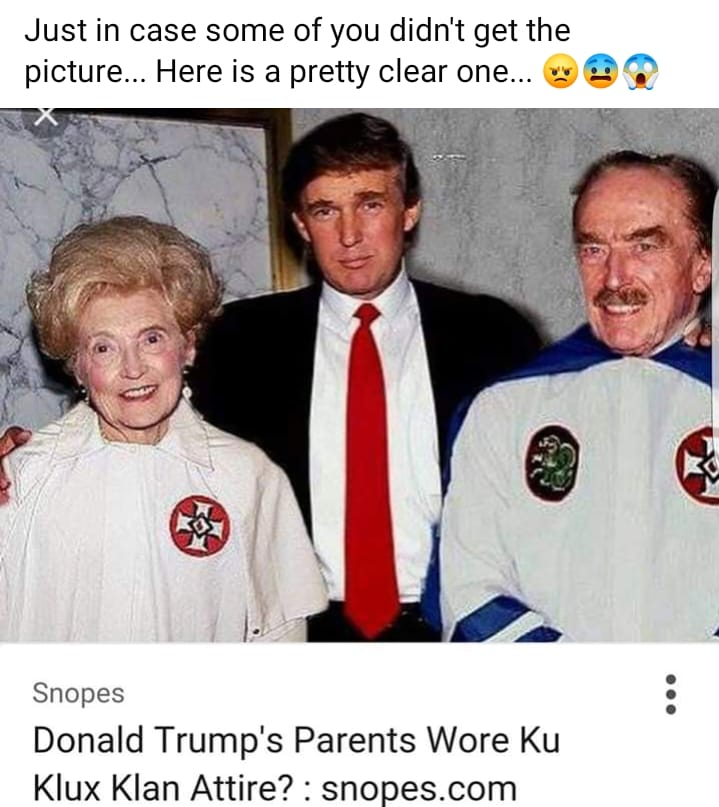
\includegraphics[width=\linewidth]{trumpkkk3.jpg}
  \caption{Version 3 of Edited Trump Image}\label{fig:TrumpKKK3}
\endminipage
\end{figure}


To a human, all three of these images are roughly the same, but there is sufficient distorting in each image (e.g. some have removed pieces of the "shutterstock" watermark, others all of them; sections of the images have been cropped or stretched or mirrored; colors have been adjusted; etc.) combined with the variations in the text around the image to confuse a CNN. Facebook even admits that their CNN struggles to tell the difference between near-identical images and that there could be "thousands or millions of copies" of these undetected near-duplicates of already flagged content \cite{sumbaly2020using}. Their new solution, "SimSearchNet", is built specifically to solve this issue, but it is not fully effective yet. Avaaz, an activist organization with a focus on stopping the spread of fake news, found that 42\% of the misinformation content they analyzed in October was currently circumventing Facebook's policies. Even more disheartening, they were able to identify 738 posts that were not labeled as fake, in spite of having already been debunked, and had collectively racked up 5.6M interactions and 142M views \cite{schott2020brief}.

Some of these had the potential to influence the 2020 election, in spite of the extra measures Facebook and Twitter added \cite{dean2020facebook}: "While Facebook applied a contextual label to one false claim on a purple background about extra postage being required for mail-in ballots, another identical claim ran against a blue background with no intervention from Facebook. The former received 14,000 shares; the latter received 20,000" \cite{Fung2020facebook}.

Ultimately, neither of the proposed Facebook punishments are effective: reducing the ability to monetize is irrelevant for an ideological actor, and reducing the spread of an image or removing it entirely is insufficient if the same image can be recreated and re-shared so easily.

\subsubsection{Scale}
\label{Scale Section}
The issue of scale is not only non-trivial, but is unmentioned in the other literature on solving this issue. Attempting to crawl through every tweet and every URL posted would be an incredibly difficult task given that Facebook alone has 1.8 billion daily active users according to their Q3 2020 earnings report, with 2.54 billion daily active users of at least one tool in the Facebook portfolio (Facebook, Instagram, WhatsApp, etc.), with those numbers ballooning to 2.74 and 3.21 billion on a monthly level \cite{facebook2020q3}. Given that in 2014 Facebook generated 4 petabytes of data daily and ran 600,000 queries with 1 million map-reducing jobs when their total daily active users was 890 million \cite{bronson2015open}, a simple ratio would provide a conservative estimate that Facebook now generates at least 8.1 petabytes of data every day, with 1.2 million queries and 2.1 million map-reducing jobs. 

Many of the proposed solutions for fake news detection are RNN based, however RNNs are far too resource heavy to be successfully implemented at the necessary scale \cite{gehring2017novel, sze2017efficient}. Even transformer based attention models, like the ones suggested in the 2017 Facebook article on machine learning, require high amounts of computational power and primarily excel at tasks like language translation \cite{vaswani2017attention}. The detection of fake news is a more complex task, as a solution must not only decipher the language being used, but also interpret a representative truth value, and return a remove/don't-remove decision within a matter of hours of the initial post's timestamp.

As Liu points out in their 2019 thesis \cite{liu2019early} while examining several of the RNN's covered in the literature review section of this thesis, each RNN is topic specific. Because of that, it begins with 0 information when the misinformation topic begins and requires a great deal of time to build up enough of a base to be successfully trained and deployed. In some crisis situations, that time may not be available. This criticism holds true for the propagation models as they require too much time before they can be successfully deployed.

The GNNs mentioned in the literature review section similarly struggle with scale. Han et al.'s GNN, for example, only looks at surface level user data such as length of user name; Chandra et al.'s GNN looks at who is consistently sharing misinformation, but it is topic specific as well and requires an extensive history of historical misinformation sharing; Nguyen et al's GNN creates only two homogeneous graphs - one looking at news sources and one looking at users - which misses the clear connections between the patient zeroes and the spread of a disease.

Along this same line of thinking, neural networks are only as useful as their training data set. Every single neural network discussed here is therefore "hack-able" at the point that individuals determine the pattern being used to allocate a post into a remove/don't-remove bucket. Several of these neural networks include surface level data like length of user name -- if a malicious actor discovers that their disinformation is being flagged simply based off of user name length, all they have to do is change their user name and their content is allowed to flow freely. Based on Eqs. \ref{trollpartisanship} and \ref{peopletoextremes}, malicious actors are attempting to push networks towards extreme partisan views; whether they're doing it for ideological, financial, or other reasons, they are incentivized to find ways to circumvent the fact-checking process. These neural network solutions are far too easy to circumvent as is (see the variations of Fig. \ref{fig:Trump Shutterstock Image} vs Figs. \ref{fig:TrumpKKK1}, \ref{fig:TrumpKKK2}, \ref{fig:TrumpKKK3}) and will only be easier as disinformation campaigns become more sophisticated. This would require every one of these neural networks to be re-trained on an iterative basis. That is time-consuming and will always have lag -- it is a reactive instead of proactive solution.


As Facebook's digital footprint grows, a successful solution must be able to grow with it and must not be easily circumvented. 



\subsubsection{Summary}
\label{sec: summary with issues with current solutions}
To summarize, the issues with the current solution are:
\renewcommand{\labelenumii}{\Roman{enumii}}
\begin{enumerate}
\item The preemptive solution is ineffective because users will not seek extra context
\begin{itemize}
\item Users will not seek extra context and will reject being prompted to look for extra context
\end{itemize}
\item An outside individual must report the post for further actions
 \begin{itemize}
     \item Users are unlikely to report posts that are in line with their partisan views
     \item Individual partisanship is strongly influenced by the beliefs of their network, which can be infiltrated by extremist ideology
     \item Extremist ideology on either side of the political spectrum is strongly resistant to fact checking, and maintaining beliefs that are opposed to generally accepted facts can actually be seen as proof of strong beliefs
    \end{itemize}
     \item After the post is reported, then it is  sent to 3rd-party fact checkers for verification. 
     \begin{itemize}
         \item Third party fact checkers are subject to the same biases as users
         \item There is no appeals process, so punitive flagging is possible
         \item Apolitical fact checkers are leaving or no longer active
     \end{itemize}
     \item Third party fact checkers must log in to the Facebook dashboard and then provide a link proving the story is false (they cannot simply mark a story as untrue).
     \begin{itemize}
         \item The process is manual and time consuming
         \item The payment from Facebook is insufficient for the time required to do the job correctly
     \end{itemize}
     \item Routine offender domains see decreased visibility, loss of advertising rights, and inability to monetize
     \begin{itemize}
         \item Loss of advertising rights is irrelevant to non-financially driven bad actors
         \item Decreased visibility (or removal) is easily circumvented by providing simple tweaks to the text or image
     \end{itemize}
 \end{enumerate}
 
\subsection{Alternative Solution: Flatten the Curve}
\label{Flatten the Curve Section}
 Most of the work detailed has been focused on trying to create a machine learning algorithm that can separate posts into a binary $\tau \in \{0,1\}$, yet, as shown in the appendix on truth values (\ref{truthvalueappendixsummary}), for the majority of posts that are not hate speech, spam/bot related, or science misinformation the actual truth value is $\tau \in \mathbb{R} \ | \ 0 \leq \tau \leq 1$. Forcing $\tau$ into a binary does a disservice to everyone involved. As discussed when comparing Bernie Sanders's tweet (fig. \ref{fig:Bernie Sanders Tweet, Oct 13, 2020}) and  Charlie Kirk's tweet (fig. \ref{fig:Charlie Kirk Tweet, May 4, 2020}), neither of those statements should have a truth value equal to 0 or 1, but neither should their truth values be equal to each other. Therefore any kind of \{0, 1\} regression or classification is fruitless and ultimately working in the wrong direction. Similarly, as illustrated in \ref{hyperbole}, there are currently no solutions that show similar results when tested on completely unique data sets of irony/hyperbole/sarcasm. Therefore, there is a high probability that ironic, hyperbolic, and sarcastic tweets would also be set to $\tau = 0$ and be flagged for removal, when they should not be. Machine learning is not the right tool to solve this problem. 
 
 Instead, this thesis proposes an alternative way of viewing this problem: a virus that needs to be curbed. The similarities are clear and even baked into our own language on the topic -- when a social media post spreads rapidly, it's called "viral". Just as not every disease is as dangerous, spreads as rapidly, or has the same life span, so too with strains of misinformation.
 
 By examining misinformation as an epidemic, the focus shifts from an ML classification problem, to aiding the doctors that can diagnose and resolve the disease: the fact-checkers. In \ref{Third Party Fact Checkers Sections}, evidence was presented that high quality fact-checkers are leaving because the platform is too cumbersome. There are simply too many posts to comb through, they have to keep rechecking identical posts (as the CNN isn't catching that they're the same), and they are not paid commensurate with the time required to do the work. While Zuckerberg proposed to use AI to handle the misinformation categorization, a better solution is to view this as an optimization problem: how can a fact checker's time be maximized? 
 
 \subsubsection{Universal Fact-Checking vs. Proportional Fact-Checking vs. Targeted Fact-Checking}
 The current solution works as a de-facto universal fact-checking: there is no threshold that must be met before the two-step solution is implemented. The machine learning solutions discussed in \ref{sec: literature review} also propose a universal "always on" fact checking solution. In analysis of viral spread, this universal fact checking is akin to "uniform immunization", where immunized individuals are entered into the population. This solution is completely ineffective as it reduces the spread of the disease too slowly, and it is impossible to determine a minimum fraction of individuals who need to be immunized in order to ensure that the infection dies off, unless every single individual becomes immunized \cite{pastor2002epidemic,pastor2002immunization,anderson1992infectious}. In order for a uniform fact-check to work, upwards of 80\% of all tweets would have to be fact-checked \cite{may1984spatial,hethcote2014gonorrhea,hethcote2013modeling,hethcote1987epidemiological,albert2000error, pastor2001epidemic}, as a network can remain contagious even after the majority of nodes are removed \cite{cohen2000resilience}. Indeed, in this context, the fraction of users $v_c$ that would need to be immunized/vaccinated and removed in order to make the network no longer contagious, $v_c \rightarrow 1$ \cite{cohen2003efficient,strogatz2001exploring,albert2002statistical,dorogovtsev2002evolution,pastor2002immunization}.
 This means that all tweets would have to pass through a fact-checking process before they could be made live, which is an impossibility at current scale and would completely destroy the business model of social networks (section \ref{Scale Section}).
 
 An alternative solution may be a proportional fact-check, where the fraction of tweets to be fact checked is proportional to their relevance in the network. For example, since there were twice as many right leaning trolls as left leaning trolls in the IRA data set \cite{freelon2020black,badawy2018analyzing,benkler2018network}, conservative content should be checked twice as frequently (or, as will be discussed in \ref{sec: Background on Networks}, Eq. \ref{powerlaw} could be used to determine proportionality based off of the number of connections).
 
 This solution too runs into myriad problems. First, it does not resolve the issue of fact-checkers having to sift through unimportant content. In a 2018 analysis of over 700 million tweets, Mention discovered that while the mean number of retweets is 1,696, the median is 0 \citep{mention2018twitter}. In other words, the average tweet is a dead end that will not spread. By proportionally allocating attention based off of partisanship, or even connectivity, fact checkers will end up spending a great deal of time confirming or disproving content that nobody will likely see. This is akin to sending epidemiologists to vaccinate hermits and ignoring the metropolis. 

Second, while proportional immunization is more effective than uniform immunization, it is not the most efficient solution \cite{dezsHo2002halting,anderson1992infectious}. The fraction needed to immunize, $v_c \approx \frac{1}{3}\lambda^2$, where $\lambda$ is the rate of spread of a disease \cite{pastor2002immunization,barabasi1999emergence}. This is better than $v_c \rightarrow 1$, but not ideal. This is because networks like the ones examined here are incredibly resistant to the loss of random nodes and are able to recover quickly \cite{cohen2001breakdown,callaway2000network,albert2000error}.

Instead, an ideal solution must be targeted in approach.
 
 
 
 \subsubsection{Proposed Solution}
 \label{sec: proposed solution}
 
 As just discussed, not all users are equally important, nor are all posts are equally important. As Grinberg et al. confirmed, only 1\% of users accounted for 80\% of the total exposures to fake news posts in the 2016 election and only 0.1\% of users (approximately 57,000) accounted for 80\% of the total shares of fake news posts in the 2016 election \cite{grinberg2019fake}. % Zooming out, primary URLs (a URL that is generated by a news source and is disseminated from an official news account) account for 2\% of the total URLs on a topic and generate 39\% of the total clicks on a topic. Secondary URLs (a URL that is \textit{not} from a primary news source from an official news account), however, generate the majority of total clicks on a topic. Slightly less than 7\% of these secondary URLs capture 50\% of the total click traffic. Combined,% 
 On a URL level, 9\% of the total URLs on a topic generate 90\% of the total click traffic (half of those are from primary news sources, the other half from secondary sources) \cite{gabielkov2016social}. 
 
 The ideal solution, then, is to treat this is a ranking problem: rather than create an RNN that checks \textit{all} tweets, only the most important 9\% need to be checked. Many other applications of network theory that focus on immunizations also illustrate that the removal of just a fraction of the total nodes can cause the entire network to disintegrate \textit{if} those nodes are intentionally and correctly selected  \cite{albert2000error,cohen2003efficient,helleringer2007sexual,cohen2001breakdown,hethcote2014gonorrhea}. Even with a scale-free network like social media, this solution will be effective. While scale-free networks are very resistant to random attacks \cite{albert2000error,callaway2000network,cohen2000resilience}, that resistance is negligible if the attacks are targeted on the most important nodes.
 
 For the set of tweets that must be fact-checked, we can assign a binary decision operator $f \in \{0,1\}$, where a tweet that must be fact checked has $f_i = 1$ and one that does not need to be (or has already been checked and approved) has $f_i = 0$. With the set of tweets to be fact-checked, $F$:
 \begin{equation}
 \label{Factcheckset}
 F=\{t_1, t_2, t_3 ... t_n \ |\ f_i \neq 0\}: F \subset T
 \end{equation}
 where each tweet in the set can be ordered by importance, such that for tweets $t_i$ and $t_j$: $t_i \succ t_j$. To determine this ranking, $\forall t \in T, \exists \  \zeta$, such that 
 \begin{equation}
    \label{zeta function}
     \zeta = \sum_{n=0}^{|A|} \beta_{n} \cdot \mu_{n}
 \end{equation}
 Where $\mu \in \mathcal{M} | \mathcal{M} \in \mathbb{R}$ is the set of relevant numerical metrics available for each user/tweet combination and $\beta \in B| B \in \mathbb{R}$ is the set of unique weights per metric. 
 
 Therefore for tweets $t_i$ and $t_j$: 
  \begin{equation}
  \label{ranking equation}
      \zeta_i > \zeta_j \Rightarrow t_i \succ t_j : t_i, t_j \in F
  \end{equation}
  
  $t^*$ is therefore the tweet that must be fact checked first, meaning  $t^* \succ \{t_1, t_2, t_3 ... t_{n-1}\}$. 
  
  Finally, the goal here is not to minimize $|F|$, as the number of tweets that need to be checked will change dynamically from moment to moment based on surrounding context. Instead, the goal should be to generate an ordered set $F^*$:
  \begin{equation}
      F^* = (t^*, t_1, t_2 \cdots t_n), \ t^* \succ t_1 \succ t_2 \cdots \succ t_n
  \end{equation}
  This allows for the fact that there will always be more posts that need to be checked than can be physically checked in a day, but also ensures that the most dangerous -- the "super-spreaders" -- are stopped first.
  


\section{Network Theory}
\label{sec: Background Definitions}
Before continuing on how to determine the appropriate metrics and weights so as to fit equation \ref{ranking equation}, it is necessary to understand how networks are built and how epidemiological spread occurs. Some of this has already been alluded to in previous sections, but this will clearly define the terms and processes.

\subsection{Background Definitions}
For these sets, the language will be that of Twitter (tweets, following, hashtags, etc.) yet the terms are easily translated to other social media groups such as Facebook, Instagram, etc.

First, for any user in the set of all users, such that $u_n \in U$, there exists a "network", $n_n \in N$ which consists of all the other users that $u_n$ follows or is followed by. This can be further parsed out into $Y_n$, the set of users who follow this user, and $Z_n$, the set of users who are followed by this user. This means that  $N_n = Y_n \cup Z_n$. 

Typically, the number of connections in the network $k_n$, is $k_n = |N_n|$. $k$ is directionally agnostic, such that $k_{ij} \equiv k_{ji}$. For this analysis, however, directionality is important: if $u_i$ followers $u_j$, there is no implication of a reciprocal relationship. Therefore, when directionality is important, this thesis will use $\Psi_n$, where $\psi_{ij}$ represents user $i$ following user $j$:
    \begin{equation}
    \begin{split}
    \label{Psi Equation}
        \psi_{ij} \in \Psi, u_j \in Z_i: i \neq j \\
        \psi_{ji} \in \Psi, u_j \in Y_i: i \neq j 
    \end{split}
    \end{equation}
However, this thesis is primarily focused with how many users follow a particular user, not how many users they follow. Therefore, let $\psi$ \textbf{only} represent inbound connections such that $\psi_{ji} \in \Psi, u_j \in Y_i: i \neq j$.

$A_n$ then becomes the adjacency matrix for network $N_n$:
    \begin{equation*}
    \label{adjacencey matrix}
\Psi_n \subset \Psi, \exists A_{i,j} = 
\begin{pmatrix}
\psi_{1,1} & \psi_{1,2} & \cdots & \psi_{1,j} \\
\psi_{2,1} & \psi_{2,2} & \cdots & \psi_{2,j} \\
\vdots  & \vdots  & \ddots & \vdots  \\
\psi_{i,1} & \psi_{i,2} & \cdots & \psi_{i,j} 
\end{pmatrix}, 
\end{equation*}
    

For clarity's sake, the terms \textit{user}, \textit{node}, and \textit{vertex} will be used interchangeably in this thesis, as will the terms \textit{follow}, \textit{connect}, and \textit{edge}. Since the direction in twitter is significant (A following B does not imply that B follows A), \textit{follow this user} will also be called \textit{in} and \textit{followed by this user} will also be called \textit{out}.


\subsection{Background on Networks}
\label{sec: Background on Networks}
This thesis will focus on Facebook and Twitter, both of which are \textit{scale-free networks} \cite{aparicio2015model,broido2019scale,barabasi2000scale} since they are networks with very few well connected nodes, called hubs, and mostly unconnected nodes \cite{barabasi2009scale,barabasi1999emergence,dorogovtsev2002evolution}. The probability of one node (here a user, \textit{u}) being connected to some large number of other users, $k$, in comparison to the average number of connections, $\langle k \rangle$, is: 
\begin{equation}
\label{powerlaw}
    P(k) \sim k^{-\gamma}, 2 < \gamma \leq 3
\end{equation}
In comparison, small networks tend to have uniform distribution of \textit{k}, such that $k \cong \langle k \rangle$: in other words, everyone is friends with everyone \cite{erdHos1960evolution,watts1998collective}.

Aparicio, et al. confirmed that Twitter followed the power-law distribution and found that for an average user $U_n \subset U:\langle | Y_n| \rangle \leq 100, \langle | Z_n| \rangle \leq 1,000, \langle \frac{|Y_n|}{|Z_n|}  \rangle \approx 0.1$. This very low ratio of in to out tracks with other research on networks which show that an individual's contacts are likely to be more connected than they are. This observation spans social networks such as friendship, computer virus spread, STD transmission, etc. \cite{feld1991your,newman2003ego,pastor2001epidemic,pastor2002epidemic,pastor2015epidemic,helleringer2007sexual,hethcote2014gonorrhea,liljeros2001web}.

On the other hand, for hub nodes $U_h \subset U: \langle | Y_h| \rangle = 67,622, \langle | Z_h| \rangle = 47,351, \langle  \frac{|Y_h|}{|Z_h|} \rangle \approx 1.43$. This hub sub-network was generated by minimizing the number of edges to connect all nodes with each other, which led to $U_h \subset U, |U_h| = 1,000$, which represented only 0.002\% of the total set of users. This is in line with the Barab{\'a}si-Albert's preferential attachment equation, with the probability, $P(\cdot)$, that a new node to the network connects to node $i$ depends on the degree $k_i$, where $j$ are all the other pre-existing nodes:
\begin{equation}
\label{preferentialequation}
    P(i)=\frac{k_i}{\sum_{j} k_j}
\end{equation}
since $\sum_{j} k_j$ is constant for any network at the instant of a node's choice, the likelihood, $L(\cdot)$, that a node new to the network chooses to connect to unique node $i$ over unique node $j$ is (with $a \succ b$ representing that $a$ is preferable to $b$) :
\begin{equation}
\label{likelihood equation}
    L(i \succ j)=\frac{P(k_i)}{P(k_j)} = \frac{k_i}{k_j}
\end{equation}

\subsection{Clustering \& Randomness}
\label{sec: Clustering}
As was discussed in \ref{sec: echo chambers}, social media users are more clustered than would be expected from a random network. The expected Barab{\'a}si-Albert clustering coefficient for user $u_i$ is the ratio of connections for that user's neighbor, $u_j$ over the total possible connections:
\begin{equation}
\label{clustering equation}
    C_{i}=\frac{|\{\psi_{jk}: u_j,u_k \in N_i, \psi_{jk} \in \Psi\}|}{k_i(k_i -1)}
\end{equation}

For an entire network, this clustering coefficient is the average of all the individual clustering scores for all users:
\begin{equation}
    C_{network}=\frac{1}{|N|}\sum_{i=1}^{|N|}C_i
\end{equation}

If a network is purely random, then the expected clustering coefficient would be:
\begin{equation}
    C_{rand} = \frac{\langle k \rangle}{n}
\end{equation}

Given Arapacio's twitter data set, if the null hypothesis, $H_0$, is that Twitter is a random network then the value for the random cluster should be the actual result. Instead, the actual result is much greater. This set has $1963 \times 10^6$ connections and $51.22 \times 10^6$ nodes, for a $\langle \psi \rangle = 38.3$:
\begin{equation}
    \begin{split}
    C_{rand} = \frac{38.3}{51.22 \times 10^6} = 7.48 \times 10^{-7} \\
    C_{actual} =\left( \frac{1}{51.22 \times 10^6}\sum_{i=1}^{51.22 \times 10^6}C_i \right)= 0.096
    \end{split}
\end{equation}
Since Twitter is a directional network and there may be reciprocal relationships, such that for user \textit{i}, $|\Psi_i| > k_i$, $7.48 \times 10^{-7}$ should be considered the lowest possible value. Even if one were to assume all relationships were reciprocal ($\forall \psi_{jk}\  \exists \ \psi_{kj}$) and cut that value in half -- which would likely overstate the number of reciprocal relationships -- the resultant value of $3.74 \times 10^{-7}$ is still 250,000 times smaller than the actual calculated result. Therefore, the null hypothesis $H_0$ should be rejected. The relationships of following and followed are not random; they are clustered and intentional.

This is further born out with the calculated $\gamma$ values. In a random network that follows the power law equation (equation \ref{powerlaw}), $\gamma = 3$ \cite{barabasi2000scale,pastor2001epidemic}, yet here $\gamma_{in} = 2.2$ and $\gamma_{out} = 1.9$. The lower $\gamma_{out}$ value can be directly traced to the evidence that individuals are likely to follow 10 times as many other users as they are followed by, which leads to hub nodes becoming more connected than would be expected in a purely random scale-free network. This also correlates to the insights from equation \ref{likelihood equation}, namely that new nodes connect with the most popular current nodes, and the "rich get richer".

Even though $\gamma_{out}$ is below the threshold of 2 initially proposed by Barab{\'a}si's and Albert's work, there are other formulations of the power-law distribution \cite{ichinose2017invasion,albert1999diameter,mislove2007measurement,zhang2015exactly,pastor2002epidemic}, which only require $\gamma > 1$. 

\subsection{Proposed Adjustments to P($\cdot$) and L($\cdot$)}
As of yet, no literature has attempted to combine the Barab{\'a}si-Albert preferential equation, equation \ref{preferentialequation}, with the partisanship analysis performed in \ref{Partisanship Section}.

Let the null hypothesis $H_0$ be that partisanship has no bearing on the preferential attachment equation, and let $H_\alpha$ be that it does, so that for user $u_n$ deciding between two other users $u_i$ and $u_j$, $\rho_{\Delta}$ will be the absolute value of the difference between these two partisanships (i.e. $\rho_{\Delta} \in \mathbb{R} \ |\  0 \leq \rho_{\Delta} \leq 1$, where 0 means complete agreement and 1 means complete disagreement. There are situations where $\rho_{\Delta}$ is undefined if the potential hub is non-partisan in nature -- these sources, such as celebrities, athletes, or apolitical news sources would be white-listed and removed, as will be discussed in \ref{sec: white listing}). Including $\rho_\Delta$ into equation
\ref{likelihood equation}:
\begin{equation}
\label{Ldotpartisan}
        \tilde{L}(i \succ j)=\frac{k_i(1-\rho_{\Delta_i})}{k_j(1-\rho_{\Delta_j})},\rho_{\Delta_j}\neq 1 
\end{equation}

If $\rho_{\Delta_j} = 1$, then it should be self evident that $i \succ j$, regardless of $i$'s partisanship; if $\rho_{\Delta_i} = 1$ \textit{and} $\rho_{\Delta_j} = 1$, then the user is stuck between two unpalatable solutions and is as likely to pick either of them as to pick neither and become a hermit. 

By extension, if equation \ref{Ldotpartisan} is accepted, then an adjustment to P($\cdot$) is necessary as well:
\begin{equation}
\label{Pdotpartisan}
        \tilde{P}(i)= \frac{k_i(1-\rho_{\Delta})}{\langle k \rangle  (1-\langle\rho_{\Delta}\rangle) }
\end{equation}
Both of these equations are logical converses to the accepted Hopfield equation \ref{macy equation}. While Macy et al. move from equation \ref{macy equation} to an examination of the probability that a user will change their mind based on the social pressure surrounding a particular topic so as to maintain a social balance and minimize dissonance \cite{macy2003polarization}, it also logically follows -- building on the same works \cite{kitts1999structural,heider1982psychology,cartwright1956structural,hopfield1982neural,hopfield1985neural,nowak1998toward} -- that a person in balance will seek to stay in balance as they add nodes to their network. In other words: partisan inertia.

If $\langle \rho_{\Delta} \rangle$ is unknown, as is a likely scenario,  0.5 can be used in the denominator of \ref{Pdotpartisan} instead. This is because $1 - \rho_{\Delta}$ effectively measures the distance in partisanship away from the center, which would make an average set of neutral content $ 1 - \langle\rho_{\Delta} \rangle = 0.5$. The reason for setting $ 1 - \langle\rho_{\Delta} \rangle = 0.5$ instead of setting it to undefined or 1 is that a user is likely to connect with someone of their own partisanship, even if their $k < \langle k \rangle$. For proof of this, Mosleh, Martel, Eckles, and Rand performed an experiment where they created an identical Twitter bot, but changed the background picture and headline to be strongly left, neutral, or strongly right presenting (fig.\ref{fig:Mosleh Image}).
 \begin{figure}[htp]
    \centering
    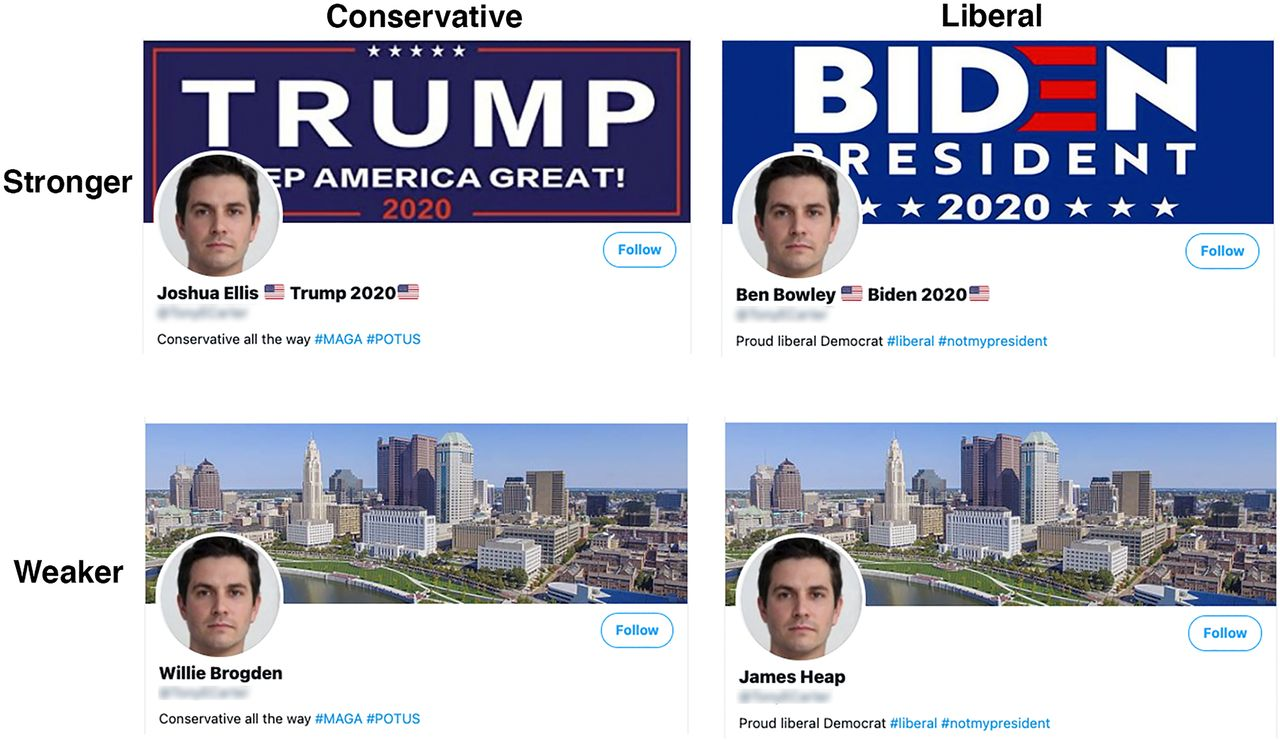
\includegraphics[width=12cm]{mosleh_image.jpg}
    \caption{Image From Mosleh et al. Experiment \cite{mosleh2020shared}}
    \label{fig:Mosleh Image}
\end{figure}

They then followed random users on Twitter who had retweeted either an MSNBC or Fox News story, and observed how many users followed them back. They found "evidence of a positive three-way interaction between co-partisanship, bot partisanship strength, and user partisanship strength" \cite{mosleh2020shared}, with no difference between highly partisan Democrat and highly partisan Republican activity. Clearly, strong displays of partisanship have value even when looking at a bot with a disproportionately small $|\psi|$ value.

At the same time, by using the average partisanship spread of the network (when known), the results are more precise and can come into better focus. They also help explain the "unlikely ally" in "enemy territory" scenario: someone with $\rho = 0$ in a community of $\langle \rho \rangle=1$ will prefer to connect with a $\rho = 0.75$ if they are the closest possible value, even though they might never connect with a $\rho = 0.75$ in any other situation. This is illustrated in the shifts in fig. \ref{fig:115th House} and fig. \ref{fig:116th House}, where representatives with deep political disagreements clustered together on key ballots.

This hypothesis breaks down into two sub-hypotheses: \\
\textbf{$H_1$}: There is a statistically relevant relationship between followers and partisanship, such that more extreme partisanship is rewarded with more followers \\
\textbf{$H_2$}: There is a statistically relevant relationship between the members of the set of followers and the partisanship of the user.

 \subsubsection{$H_1: k \propto |0.5 - \rho|$}
  \label{$H_1: k \propto |0.5 - \rho|$}
 To test $H_1$ the Twitter follower count of each representative in the 116th congress was attached to their voting records by accessing the Twitter API using the \textit{Tweepy} library. For representatives with multiple accounts, the account with the higher number of followers was selected and representatives without a Twitter account were removed from the data set. 

A $\chi^2$ test was then performed on the Republican representatives, as the kurtosis of partisanship for the Democratic members was almost four times that of the Republican members -- 97 of the 236 Democratic Representatives tracked were within two votes of each other during the entire session, so there would be no statistically relevant relationship between voting pattern and followers. However, for Republicans ($n = 199$), the $p$-value for this test was $p=0.0005$. Therefore we can say that -- for Republicans in the 116th congress at least -- the null hypothesis should be rejected, and we should conclude that there is a relationship between twitter followers and voting patterns. This confirms that 0.5 is an appropriate value in equation \ref{Pdotpartisan}.

\subsubsection{$H_2: \rho \Rightarrow Y$}
\label{$H_2: \rho \Rightarrow Y$}
To test $H_2$, that the partisanship maps to the set of followers, two members of the 116th house with similar twitter follower sizes were selected: Rep. Devin Nunes, who had 1,272,026 followers as of 1/10/20, and voted in line with Trump 93\% of the time and Rep. Rashida Tlaib, who had 1,332,772 followers as of 1/10/20, and voted in line with Trump 12\% of the time. With $Y_t$ be the set of followers of Tlaib and $Y_n$ the set of followers of Nunes: 
\begin{equation}
\frac{|Y_t \cap Y_n|}{|Y_t \cup Y_n|} = 0.0028 = 0.28\%
\end{equation}
From a random set of 5,000 followers of each representative (which would give an $\alpha = 0.01$ and a confidence interval of $\pm 1.8\%$), there were only 28 followers in common.

In comparison, Rep. Ilhan Omar, who voted with the President 11\% of the time and has 2,810,605 followers, had a similarity score of 8.4\% to Rashinda Tlaib. Rep. Kevin McCarthy, who voted with the President 95\% of the time and has 1,175,068 followers, had an 11\% similarity score to Devin Nunes.

This experiment was repeated with the top 5 members of each party of the 116th congress by twitter followers: Democrats Lewis, Pelosi, Ocasio-Cortez, Tlaib, and Omar, with $Y_D$ as the union of the sets of the 5 Democrats' followers; Republicans Nunes, McCarthy, Jordan, Gaetz, and Crenshaw with $Y_R$ as the union of the sets of the 5 Republicans' followers:
\begin{equation}
\label{party overlap twitter}
    \frac{|Y_D \cap Y_R|}{|Y_D \cup Y_R|} = 0.0108 = 1.08\%
\end{equation}

Given the low Jaccard indices for cross-party followers, even when looking at 10 representatives together, and a higher intra-party index, we must reject the null hypothesis that there is no correlation between party affiliation and follower similarity scores. Indeed, \textbf{there is at least 8x more overlap in followers of the same party than across parties}. This ties back to the previously illustrated examples of \textit{echo chambers} and the experiment of Mosleh et al., referenced earlier \cite{mosleh2020shared}.

\subsubsection{Summary}
\label{sec: P dot summary}
Since both $H_1$ and $H_2$ are accepted, the proposed adjustments to $L(\cdot)$ and $P(\cdot)$, equations \ref{Ldotpartisan} and \ref{Pdotpartisan}, are accepted.

At first glance, this analysis comes into conflict with the individual clustering coefficient equation used for combining hierarchical structures with modularity in real networks \cite{ravasz2003hierarchical,dorogovtsev2008critical,dorogovtsev2002pseudofractal}:
\begin{equation}
\label{hierarchy equation}
    C(k) \sim k^{-1}
\end{equation}
This equation, where a high $k$ value implies a low clustering coefficient implies that the more connections a node has, the less clustered that group will be. This is found to be true in networks from film actors on IMDB \cite{amaral2000classes,albert2000topology,barabasi1999emergence} to language webs where words are treated as "connected" if they are listed as synonyms in the Merriam-Webster dictionary \cite{sole2001small,yook2002modeling,sigman2002global,dorogovtsev2001language}. In the case of IMDB, the majority of actors had very low $k$ values (as they were only in one or two films) and thus had a high clustering coefficient (everyone else in the film was also only those one or two films); however, there were a handful of performers with large $k$ values whose careers spanned many films in many genres across many decades -- the Jack Nicholsons. 

However, it is important to recognize the importance of modularity and hierarchy here. In most scale-free networks, small sub-networks have very densely connected nodes and hubs tend to bridge those gaps, but in hyper-partisan environments, that task may be too difficult to achieve. This $C(k)$ equation will hold true globally for users that should be white-listed as will be discussed in section \ref{sec: white listing}, but for these smaller more partisan arenas, there is no cross-partisan hierarchy. 

\subsection{Proposed Adjustment to the Average Partisanship Equation}
As shown in equation \ref{Ldotpartisan}, there is a correlation between partisanship and similarities in the sets of followers, validating the hypothesis of the existence of echo chambers. However, it also illustrates that a new user will find $u_i \succ u_j$ based off the combination of relative partisanship and current followers. It therefore follows that equation \ref{ech chamber} should similarly be adjusted: as it stands, it implies that all partisanship is equally weighted when determining the average partisanship of the network, yet equation \ref{likelihood equation} shows that they are not: hub nodes carry more weight than non-hub nodes. This combination provides:
\begin{equation}
    \label{echo chamber by followers}
        \langle \rho_n \rangle = \frac{\sum_{i=1}^{|n_n|}\rho_ik_i}{\sum_{j}k_j}, (u_i \in n_n, n_n \in N)
 \end{equation}
 
 The partisanship of a hub node, $k_i > \langle k \rangle$, has an out-sized influence on the partisanship of the network. People who fall into this group will be called \textbf{macro-influencers} in this thesis.
 
 A node that is \textit{not} a hub node, $k_i \leq \langle k \rangle$, yet is still having an out-sized influence in the conversation, such that for the set of tweets on a particular topic, $T_t$, the interactions, $i_i$ for their tweet $t_i \in T_t$ has the property $i_i > \langle i \rangle, t \in T_t$, would be called a \textbf{micro-influencer}. They have the \textit{micro-} prefix because their influence is currently limited to this particular topic, whereas a hub node is likely to be a hub node in all scenarios.

\section{Metrics For Ranking Function}
\subsection{Four Proposed Metrics}
This thesis proposes that the seven W's ("Who", "What", "Where", "When", "Why", "How", and "With What") that come from Aristotle \cite{sloan2010aristotle,aquinas1952thomas} be the basis of this thesis. Of these seven, three are self-evident or irrelevant: the "where" is social media; the "by what means" and the "why" are not relevant to our examination. As discussed previously, unintentional or unverified rumors are just as dangerous as intentional misinformation; similarly, whether misinformation comes from a paid source or an ideological source has no bearing on how dangerous it is. Therefore, this thesis narrows these questions down to four: Who is sharing the content, what are they sharing, how quickly is it spreading, and how far along is it?

\subsection{Who is Sharing?}
At first glance, the ideal solution is simply to focus on the hub nodes, however this requires a great deal of, if not complete, knowledge about the network in advance  \cite{dezsHo2002halting,pastor2002immunization}. That having been said, since social media users have $|Y|$ values readily available, this still seems to be an easy solution. However, the $|Y|$ value of a "hub node" is an inconsistent metric - at its peak, @TEN\_GOP had around 100,000 followers, but other troll accounts identified in the Mueller report had lower $|Y|$ values:

\begin{quote}
Individualized accounts used to influence the U.S. presidential election included @TEN$\_$GOP (described above); @jenn$\_$abrams (claiming to be a Virginian Trump supporter with 70,000 followers); @Pamela$\_$Moore13 (claiming to be a Texan Trump supporter with 70,000
followers); and @America$\_$1st$\_$ (an anti-immigration persona with 24,000 followers). \cite{mueller2019mueller}
\end{quote}

Based on a broad analysis of twitter as a whole, (and the average metrics provided by Aparicio et al. \cite{aparicio2015model}), the average $|Y|$ value for a hub node is 67,622. This would catch some of the troll accounts listed but not all of them. Nor would it catch Facebook groups with low numbers of highly active people: unarguably, a group with a small number of people who are constantly active is more worthy of attention than a large group where nobody is active.

This may seem like an impossible ball to untangle at first, but equations \ref{ech chamber}, \ref{peopletoextremes}, and \ref{echo chamber by followers}, illustrate that an individual's partisanship is directly related to the partisanship of the most connected person in their network. While one might argue that an individual might follow opposing view points, the results of equation \ref{party overlap twitter} show that this is statistically unlikely to be the case for $p < 0.05$. Similarly, one might argue that merely following someone does not necessarily imply $\rho_i \simeq \rho^*$, where $i$ is the unique user and $\rho^*$ is the partisanship for $u^*$, the user with the $\max(|\psi|), u^* \in Z_i$. This thesis does not deny that. However, there are key points to recall:
\begin{enumerate}
    \item Users with high connectivity and high partisanship (i.e. high $|\psi|$ values and $\rho \rightarrow 0$ or $\rho \rightarrow 1$) could be hubs for \textit{this} network, $n$, but will not necessarily have high connectivity when compared to all possible nodes or be nodes for all of Twitter (eq. \ref{hierarchy equation}) 
    \item Users who follow $u^*$ are likely to follow other similar users with similar viewpoints (eq. \ref{Ldotpartisan}).
    \item The probability that an individual follows a user who shares misinformation is not changed by the individual's reaction to the misinformation (eq. \ref{probability of infected node}).
    \item Since this thesis focuses on modeling misinformation as viral spread, there is nothing incorrect with including users who may be "immune" to the misinformation as natural immunity also occurs in traditional viral spread (eq. \ref{reduced v_c}, \ref{immunity equation}).
\end{enumerate}

Let $\vec{A_i}$ be a vector of ordered pairs of all users that $u_i$ follows and their corresponding follower counts:
\begin{equation} 
\label{row of adjacency matrix}
\vec{A_i}=\{(u_1,|\psi_1|),(u_2,|\psi_2|),(u_3,|\psi_3|)\dots (u_n,|\psi_n|)\}, u \in Z_i, \psi \in \Psi
\end{equation}

By all the equations and background discussed earlier, the most important $u \in Z$ is the user with corresponding $\max(|\psi|)$. This allows for private groups, reportedly a key place where the riot at the U.S. Capitol on January 6th was planned and misinformation was spread \cite{yin2021facebook,horwitz2020facebook}, to be included: $|\psi|$ for said group is the number of members who belong to it. 
Let $U^*$ then be the set of all users who are a $u^*$ for at least one other user.

We can then determine the number of times a particular user appears in that set, which will be the first metric: 
\begin{equation}
\label{mu_1 equation}
    \mu_1 = \sum_{u\ \in \ U^*}1_{\{u_i\}}(u)
\end{equation}

This proposed equation operates as a more refined version of Cohen et al.'s strategy for immunization: choose an individual and then vaccinate a random connection of theirs. In their modeling, they found that this strategy was able to arrest spreading viruses with only 25\% of the population vaccinated (in comparison uniform immunization required almost 100\% of the population vaccinated to see the virus end) \cite{cohen2003efficient}. They found that this model provided insight into ecological networks \cite{sole2001complexity,camacho2002robust}, metabolic networks \cite{jeong2000large}, cellular proteins \cite{jeong2001lethality}, and terrorist networks \cite{cohen2003efficient}. 

\subsubsection{White Listing}
\label{sec: white listing}
One of the helpful parts of this particular dilemma is that a great deal of information is known about \textit{some} members of the network. Some users with a very high $|\psi|$ value are known news outlets, comedians, sports organizations, etc. which do not require the same level of scrutiny that other accounts do. Users where $\rho_{\Delta}$ is undefined can be whitelisted and removed from this set. This list can have an established cadence for review, so that celebrities who begin tweeting misinformation (as in the cases of actor Woody Harrelson, UK boxer Amir Khan, and US rapper Wiz Khalifa tweeting about 5G causing COVID \cite{bruns2020covid19}), can have their white-listed privileges revoked. 

If a user is in this set of white listed users, then they would be removed from $\vec{A}$ for all users, thus preventing from being considered a $u^*$.

\subsection{What is Being Shared?}
\label{sec: what is being shared}
Currently, Twitter, Facebook, and other social media companies label topics as \textit{trending} (fig. \ref{img:Trending Topics}), which is based almost exclusively on kurtosis over a very small window of time \cite{dewey2015freddie,lotan2015freddie}. 

\begin{figure}[htp]
    \centering
    
\includegraphics[width=6cm]{Twitter Trending.png}
    \caption{Trending Topics on Twitter, Jan 30 2020}
    \label{img:Trending Topics}
\end{figure}

When the elapsed time from a post's creation to the moment of inspection, $j$, is sufficiently small, it's possible to draw incorrect conclusions about the actual velocity of the content. Trending, per Lotan, operates more akin to jerk in physics and is connected to the the number of retweets at the moment: 
\[
    \frac{\partial^3 r}{\partial j^3}
\]

There are two flaws here. First, using $r$ favors topics that may or may not quickly expire on their own while ignoring slowly growing topics. In the Washington Post article cited earlier, \#FreddieGray was never considered trending on Twitter even though the story was featured prominently on CNN, ABC, the New York Times, etc. and more than 150,000 people tweeted on the topic on April 25, 2015 (fig. \ref{img:Trendinalia 2015})
\begin{figure}[htp]
    \centering
    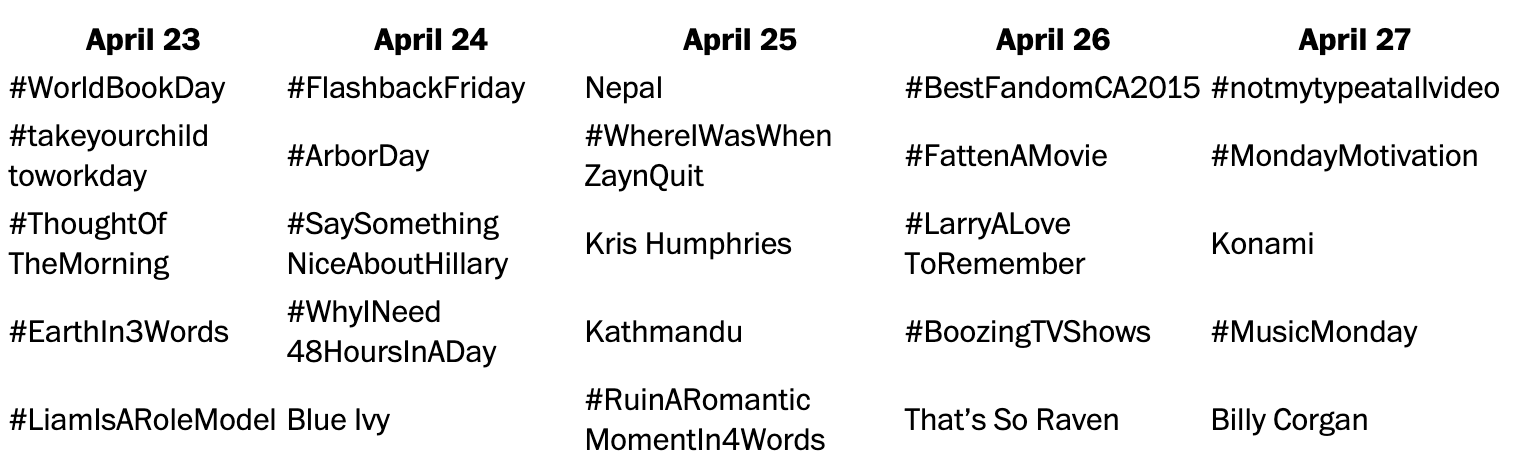
\includegraphics[width=11cm]{Trendinalia Apr, 2015.png}
    \caption{Trending Topics on Twitter via Trendinalia, Apr 2015}
    \label{img:Trendinalia 2015}
\end{figure}
. 

As Lotan, a data scientist for Buzzfeed, pointed out:
\begin{displayquote}
1. The longer a term stays in the trending topic list, the higher velocity [of tweets] required to keep it there. \\
2. It is much easier for a term never seen before to become a Twitter trend, and finally \\
3. It is extremely important to understand what else is happening in the region or network (if Kim Kardashian’s show is airing, you can forget about trending!). \cite{lotan2015freddie}
\end{displayquote}

Sociologist Zeynep Tufekci argues in multiple media that this becomes de-facto censorship \cite{tufekci2017twitter,tufecki2018democracy,tufekci2017we,tufekci2014online}. She provides numerous examples, such as Facebook's 2014 trending window which provided high visibility to topics such as the "Ice Bucket Challenge", but completely left off the protests in Ferguson, MO after the shooting of Michael Brown. This, she contends, creates effective censorship: by denying visibility to a particular topic while elevating another, social media is making (whether intentional or not) editorial decisions. 

In defense of utilizing $\frac{\partial^3 r}{\partial j^3}$ to determine whether or not a topic is trending, a high value here shows very high engagement at a particular point in time. There is nothing inherently wrong or immoral about connecting disparate groups who are all watching and commenting on a TV show at the same time. At the same time, as both Tufecki and Lotan point out, it's easy for important topics to get drowned out by noise. Certainly, there is room for improvement.

\subsubsection{Current Literature Alternatives} 
Because social media posts are filled with spelling errors, typos, abbreviations, lexical variations, etc., it is incredibly difficult to gather a precise understanding of the post in a reasonable amount of time \cite{vandam2019learning,laniado2010making,schubert2014signitrend}. Dashtipour et al. analyze how reliant text analysis is on a robust lexicon, which will always lag behind common usage of language, and some languages have more thorough lexicons than others \cite{dashtipour2016multilingual}.

VanDam, however, proposes a neural network that runs on the set of each unique user's tweets (rather than a global dictionary) to detect if a post is "out of place", which can point towards a compromised account, or if a hashtag has been "hijacked" and users are sharing unrelated or negative content with the hastag attached  \cite{vandam2019learning, vandam2016detecting}. One example of this was McDonalds using \#McDStories where users used the hashtag as an opportunity to vent about unpleasant experiences with McDonalds \cite{jain2015hashjacker}. On the other hand, both Gilkerson & Berg and Sedberg & Bennett note that hashtag hijacking can be a positive way for activists to stimulate necessary dialogue \cite{gilkerson2018social,bennett2012logic}. Finally, some examples of hashtag hijacking are unintentional blunders, such as when a pizza company tried to encourage people to stay in and eat pizza using the hashtag \#whyistayed, missing that that hashtag had been used to bring attention to victims of domestic abuse \cite{vandam2019learning}. While this solution is useful, it only detect outliers against a pattern. In examples where the hashtag is primarily being used as a beacon of disinformation, such as \#stopthesteal and \#sharpiegate were used during the 2020 election to signal election fraud \cite{perez2020facebook}, this solution would be unhelpful.

Another way to determine topic importance is to use top-k modeling \cite{babcock2003distributed}, but this solution measures \textit{volume} and not \textit{importance}, which is not a relevant metric for this thesis. 

\subsubsection{Word Pair Hashing}
This approach to content analysis borrows heavily from the insights of Schubert, Weiler, and Kriegel, who also observed that current solutions, such as TF-IDF or First Story Detection (a model to detect the first reporting of an incident \cite{petrovic2010streaming,yang1998study}), require a great deal of memory. They detected that this scaling issue gets even worse when looking at word pairs -- an alternative solution, \textit{enBlogue}, retains $2p$ historical values for any word pair, with $p$ being the number of recent occurrences of the pair \cite{alvanaki2012see} -- which leads to retaining data for at least 700 million word pairs at any given point in time \cite{schubert2014signitrend}. Given all of the unintentional and intentional issues with social media posting spelling and grammar, that number has the potential to balloon significantly. 

Instead, Schubert, Weiler, and Kriegel propose a word pair hashing system with a half-life. This half-life inclusion allows for word pairs to be removed from the set as they cease to be relevant, thus freeing up memory, but also allows for topics that grow at a slower rate not to get lost in the shuffle. Furthermore, by hashing the words, the system has no need to store any lexicographic information -- it also resolves the issues presented by Dashtipour et al.

They propose a model based off of the Exponential Weighted Moving Average (EWMA) and variance (EWMVar). By using moving average and moving average variance, this prevents topics that had a very high amount of discussion a long time ago from retaining any supremacy. 

They propose that $x$ is trending if $x$ is greater than an alerting threshold as defined by:
\begin{equation}
    \label{trending}
    x >EWMA + s \cdot EWMVar =: t
\end{equation}
 
where $s$ is the significance level. 

Let $\alpha$ be the learning rate here, such that:
\[
\alpha_{half-life} = 1 - \exp\big(\log \big(\frac{1}{2}\big)/t_{1/2}\big)
\]
with $t_{1/2}$ being the half-life time that is manually decided by the appropriate subject matter expert.
This can be combined with the equations by Finch \cite{finch2009incremental}:
\begin{equation}
    \label{Finch Equations}
    \begin{split}
        \Delta  \xleftarrow[]{}  x - EWMA \\
        EWMA  \xleftarrow[]{}   EWMA + \alpha \cdot \Delta \\
        EWMVar  \xleftarrow[]{} (1-\alpha) \cdot (EWMVar + \alpha \cdot \Delta^2)
    \end{split}
\end{equation}

From here, Schubert, Weiler, and Kriegel generate $2^\ell$ buckets, each storing an EWMA and EWMVar value, and $k$ hash functions, so that each word is mapped to a maximum of $k$ buckets. The process then compares the popularity of words in the epoch vs the popularity of words already stored in the buckets, making sure that less popular word pairs do not overwrite more popular word pairs. They observe that $\ell$ needs to be large enough to ensure that the buckets aren't filled with frequent keywords. 

They tested their solution on posts about Edward Snowden's flight from Hong Kong to Moscow. At that time, posts about Snowden were already quite prevalent, so the words \textit{Edward} and \textit{Snowden} had started to drop off from their "trending" metric due to a lack of novelty, but various combinations of the word set \{\textit{edward, snowden, hong, kong, moscow}\} exhibited significant peak. Similarly, when looking at the same Boston Marathon bombing data set as Starbird et al. \cite{starbird2014rumors}, they were able to isolate when the social media conversations shifted from being generally about the Boston Marathon to being about an explosion at the Boston Marathon (the term \textit{explosion}, interestingly, had been used frequently in the days before hand as there had been a Boeing 787 Dreamliner battery explosion).

\subsubsection{Process}
The daily process and analysis would be in two parts: indexing and analyzing.

For indexing, every document will have each word pair indexed in the hash table, such that it's moving average and moving variances are recorded and updated as more frequencies of the word pairs appear. At each point, as a final step of the indexing process, the frequency of that word is measured against a maximum $z$-score ($\beta$ here is a constant to ensure that the denominator is not zero):
\begin{equation}
    z = \frac{x-\max\{\mu, \beta\}}{\sigma + \beta}
\end{equation}
If that $z > t$, the threshold for alerting, then it is immediately routed to an early alert system.

For end-of-day analyzing, both the EWMA and EWMVar tables are updated such that words with lower popularity are overwritten with new pairs with higher popularity. Terms are also analyzed for their $z$-score as calculated above here, which provides a list of terms that trended that day. Those terms are both worthy of further investigation and are potentially a warning for what will trend tomorrow.

\subsubsection{Moving Averages With Small Windows}
One of the difficulties that they observed was that this model struggles during an epoch, as the number of posts during an epoch is not known until the epoch is complete, which can over-inflate the importance of a particular word pair. However, this is a task that machine learning is uniquely suited for, as a very simple algorithm can predict the number of tweets that will be generated at a certain time in a certain country in a certain time zone. Poisson regression is likely appropriate here.

Interestingly, while Mueller's team did not use machine learning, they did observe that many of the fake posts that came from the IRA were posted at unusual times for the locations the accounts claimed to be in... but were in standard working hours in Moscow \cite{mueller2020internet}.

When compared with an average number of posts for the country and time zone these fake accounts claimed to live in, it would have been immediately clear that they were not only "trending" but would likely need to be flagged for investigation.

\subsubsection{Summary}
\label{what is being shared summary}
While there may be some value to including a set of topics that are white-listed (much like white-listing users as discussed in \ref{sec: white listing}), this solution uses such a small amount of memory that this would be overkill and could potentially lead to content getting missed. When analyzing Twitter data utilizing a streaming API over 114 days, they captured 279 million tweets -- approximately 1\% of all tweets during that period -- which turned into 6.7GB of processed data. Processing this twitter data took, on average, 46 seconds per day; the actual analysis took, on average, 25 seconds per day; the data storage required, on average, was only 160MB per day. In fact, they ran this entire process off of a 700Mhz computer with 512MB of RAM, at a processing speed of 104.1 seconds per day \cite{schubert2014signitrend}. Clearly, this process can be applied to the full Twitter "firehose" without issue and without need for further adjustments.

Furthermore, this solution solves the problem posed at the beginning of this section where important topics with small kurtosis were drowned out and went unnoticed. Since the key words are held in tables and moving averages are used, topics with high trending but low sustainability (such as a sports event or TV event) will enter and leave the tables quickly, while topics that show low but consistent growth (such as \#FreddieGray) will remain present. 

Therefore, let $I$ be the set of trending topics as determined by the tables described previously with $i$ being a unique pair, $z$ be the $z$-score result generated from the exponential moving average/variance tables, $s$ be the significance level, and $d$ be the number of days (not necessarily consecutive) that this topic has been in the tables .

This provides $\mu_2$ which can give us the importance of the content being discussed:
\begin{equation}
\label{mu_2 equation}
    \mu_2 = \begin{cases}
    z\cdot d  & \text{if}\ i \in I\ \text{and}\  z > s \\
    0\  & \text{if}\ i \notin I \ \text{or} \ z \leq s
    \end{cases}
\end{equation}

As a final note here, it is worth mentioning that none of the previously discussed neural networks accounted for the fact that they would need to be perpetually trained to be effective. As seen here, moving averages are important: topics that were important yesterday are not necessarily important today. Patterns of fake news yesterday that have been identified can be easily changed to create fake news today. This is yet another flaw to the proposed self-sustaining neural network solutions.

\subsection{How Fast is it Spreading?}
\subsubsection{Standard Rate of Transmission: $\lambda$ Value}
There are many ways to determine transmission rate, $\lambda$. For this thesis, $\lambda$ will be the derivative of the cumulative sum of retweets. 

While users will unquestionably read content without retweeting it, Gabielkov et al. observed that the relationship between retweets and total followers can be used to project times that a user has seen content without sharing it \cite{gabielkov2016social}.

Therefore, let $y_j$ be the cumulative sum function $y_j = \sum_{i=o}^j r_i$ where $r_i$ is the number of retweets at that particular point in time. $y_j$ can be further understood to be a natural log function of time, based on analysis of retweet paths over time \cite{gabielkov2016social,starbird2014rumors,mention2018twitter}, such that for any tweet, the total retweets over time maps to $f(j) = a \ln j$, where $a$ is a constant. This means that the rate of change:
\begin{equation}
    \label{rate of transmission}
    f'(j) = \frac{a}{j} = \lambda
\end{equation}

\subsubsection{Standard Critical Rate of Transmission: $\lambda_c$}

Given the density equation for infected nodes $d$: \begin{equation}
    \label{densityequation}
    d \sim \exp\left(\frac{ - C}{\lambda}\right)
\end{equation} where $C$ is a constant and $\lambda$ is the rate of transmission \citep{pastor2001epidemic} (note that $d$ does not scale with the number of nodes in the network, which is typical of epidemics studied in previous literature \citep{marro2005nonequilibrium}), equation \ref{rate of transmission}  can be merged in to provide:
\begin{equation}
    d \sim \exp\left(\frac{ - C}{a}j\right)
\end{equation}

The dynamic mean-field reaction rate from \citep{marro2005nonequilibrium,pastor2001dynamics,pastor2001epidemic} as relates to $j$ for a node with $k$ connections (here $d_k(j)$ is the relative density of nodes with $k$ connections) is: 
\begin{equation}
\label{dynamic mean-field reaction rate}
    \partial_jd_k(j) = - d_k(j) + \lambda k \big(1 - d_k(j)\big)\Theta(\lambda)
\end{equation}
At this point, let $\psi$ be substituted in for $k$, as with the previous equations:

\begin{equation}
\label{dynamic mean-field reaction rate psi}
    \partial_jd_{\psi}(j) = - d_{\psi}(j) + \lambda \psi \big(1 - d_{\psi}(j)\big)\Theta(\lambda)
\end{equation}

By setting the mean field equation, equation \ref{dynamic mean-field reaction rate psi}, set to a static state ($\partial_jd_{\psi}(j) = 0$), the $d_{\psi}$ can be solved for:
\begin{equation}
\label{static d_psi}
    d_{\psi} = \frac{\lambda \ \psi \ \Theta}{1 + \lambda \ \psi \ \Theta}
\end{equation}

The probability that any particular node follows a user who shares misinformation, $\Theta(\lambda)$, is directly related to equation \ref{Pdotpartisan} :
\begin{equation}
\label{probability of infected node}
    \Theta(\lambda) = \sum_{\psi} \frac{\psi P(\psi)d_{\psi}(j)}{\langle \psi \rangle}
\end{equation}

Combining \ref{probability of infected node} with \ref{static d_psi} provides:
\begin{equation}
    \Theta =  \frac{\sum_{\psi} \psi P(\psi)}{\langle \psi \rangle}\cdot \frac{\lambda \ \psi \ \Theta}{1 + \lambda \ \psi \ \Theta}
\end{equation}

$\Theta$ clearly must be between 0 and 1, inclusive, with the $\lambda$ value that sets $\Theta = 1$ called the critical $\lambda$ value or $\lambda_c$. The critical value is that where the network will be completely overrun and every node will be infected: 

\begin{equation}
\label{critical value equation}
    \frac{\sum_{\psi} \psiP(\psi)\lambda_c\psi}{\langle \psi \rangle} = \frac{\langle \psi^2 \rangle}{\langle \psi \rangle}\lambda_c = 1 \Rightarrow \lambda_c = \frac{\langle \psi \rangle}{\langle \psi^2 \rangle}
\end{equation}

The clear question that needs to be answered next is for which network $\langle \psi \rangle$ and $\langle \psi^2 \rangle$ should be calculated. 

\subsubsection{Network Size: Partisan Immunity}
By continuing with the viral spread metaphor, users with a $\rho > 0.5$ are more likely to be immune from left-leaning misinformation and those with  $\rho < 0.5$ are more likely to be immune from conservative misinformation. Mathematically, this aligns with Macy et al.'s equation on propensity, $\pi_{is}$ for user $i$ to adopt view point $s$ where $v_s$ is a binary value on whether the user is willing to change to their mind on $s$ and $P_{is}$ is the partisan "pressure" of the network:
\begin{equation}
\label{propensity}
    \pi_{is}=\frac{v_s}{1+\exp{(-10P_{is})}}+(1-v_{s})X_i
\end{equation}

Let $\iota$ represent a function that calculates the likelihood that a user will be immune to a particular strain of misinformation, where $\rho_{\Delta}$ is the absolute value of the difference between the partisanship of the user, $i$, and the content, $s$:
\begin{equation}
\label{immunity equation}
    \iota(\rho_{\Delta})=\frac{1}{1+\exp{\big(-10 (\rho_{\Delta_{is}}-0.5)\big)}}
\end{equation}

Equation \ref{immunity equation} maintains the sigmoid function of \ref{propensity}, but it removes the variable $v_s$ as it is unnecessary when $\rho_{\Delta}$ is known. As illustrated in section \ref{sec: echo chambers}, an individual's belief structure conforms to the surrounding network. If an individual is diametrically opposed to a political opinion ($\rho_{\Delta} = 1$), then $\iota = 1$, which means they are effectively immunized against it. Much like with viral spread, individuals with $\iota = 1$ are dead-end nodes that will not spread this misinformation; individuals with $\iota = 0$ are highly susceptible to this strain of misinformation and are highly likely to spread it to others.

Utilizing the S-I-R model where nodes are categorized as susceptible–infected–removed \cite{ferrari2006network,bailey1975mathematical,newman2005threshold,newman2002spread}, it is standard to remove immune nodes from the network as they will neither transmit nor be infected by the disease. Therefore, the traditional $\langle \psi \rangle = \psi P(\psi)$ equation must now factor in immunity:
\begin{equation}
\label{psi immunized}
 \langle \tilde{\psi} \rangle =  \psi P(\psi)(1-\iota)
\end{equation}

Given the sigmoid nature, this allows for users who are not diametrically opposed to content to be included on a fractional basis: individuals with a $\rho = 0.5$ or true centrists are equally likely to be susceptible to far right or far left misinformation, yet are not completely defenseless against either.

Combining \ref{critical value equation} and \ref{psi immunized} generates $\tilde{\lambda_c}$, which now utilizes $\tilde{\psi}$.

\subsubsection{Metric and Summary}
First, the metric here will be the ratio of the rate of transmission vs. the critical rate of transmission: $\frac{\lambda}{\tilde{\lambda_c}}$, such that if this metric is $\geq 1$, then the epidemic is out of control and if $< 1$ then it will die out on its own. Note that this equation for $\mu_3$ is very similar to the probabilistic version of determining critical spread that uses $\Theta$ and $\Theta_c$ \cite{newman2005threshold,ferrari2006network,meyers2005network,callaway2000network,newman2002random}.

By combining these terms:
\begin{equation}
\label{mu_3 equation}
    \mu_3 = \frac{\tilde{\lambda}}{\tilde{\lambda_c}} = \frac{a \langle \tilde{\psi^2} \rangle}{j\langle \tilde{\psi} \rangle}
\end{equation}

By using $\tilde{\psi}$ instead of a general network wide $\psi$, $\mu_3$ allows for viral spread to be compared in a more apples-to-apples fashion: all immune and irrelevant nodes are factored out. 


%%% lambda over lambda c.... psi^2 cancel out????
\subsection{How Far Along is it?}
For this section, the primary question is how to get $\mu_3 < 1$. There are two ways to achieve this. When $j$ is sufficiently large, it can outweigh $\frac{\langle \tilde{\psi^2} \rangle}{\langle \tilde{\psi} \rangle}$. The other solution is to "vaccinate" or remove nodes from the network, which will reduce the $\langle \tilde{\psi} \rangle$ value in the numerator. Clearly, by removing as many $u^*$ from the network, the $\max |\psi|$ values are removed, which will drop the value in question. However, the purpose of this thesis is to target the nodes for vaccination/fact checking. 

The ideal relationship, then, will marry both $\psi$ and $j$ values. When $j$ is sufficiently small, the misinformation will unquestionably have $\mu_3 > 1$ as only a few retweets in rapid succession right after a tweet is posted will make a very large $\tilde{\lambda}$ value.

\subsubsection{Fraction of Users to Target}
In immunization work on network theory \citep{pastor2002immunization}, the fraction of individuals that should be vaccinated in a targeted scenario, $v$, is equal to 
\begin{equation}
    v = \sum_{k > k_t}P(k)
\end{equation}
where $k_t$ is a minimum threshold of connections and any user with connections above that threshold will be vaccinated. 

Combined with \ref{Pdotpartisan}:
\begin{equation}
\label{probability of vaccinated}
p(v) = \frac{\sum_{k>k_t(v)}kP(k)(1-\langle \rho_{\Delta_{k>k_t}})\rangle}{\sum_{k}kP(k)(1-\rho_{\Delta})}
\end{equation}

If those people are considered removed, then the new distribution would be \citep{cohen2001breakdown}:
\begin{equation}
    P_v(k) = \sum_{1\geq k}^{k_t}P(q)\binom{q}{k}(1-p)^kp^{q-k}
\end{equation}
This leads to new $\langle k \rangle_v$ and $\langle k^2 \rangle_v$ values (after cut-off introduction and link removals)\citep{pastor2002immunization}: 
\begin{align*}
        \langle k \rangle_v &= \langle k \rangle_t(1-p)\\
         \langle k^2 \rangle_v &= \langle k^2 \rangle_t(1-p)^2+\langle k \rangle_t\ p(1-p)
\end{align*}

At this point, $k$ can be replaced with $\tilde{\psi}$ (as before, inbound connections with "immune" nodes removed) to make it compatible with equation \ref{psi immunized} to determine $v_c$, the critical fraction of users who need to be vaccinated:
\begin{equation}
\label{v_c equation}
 \frac{\langle \tilde{\psi}^2 \rangle_{v_c}}{\langle \tilde{\psi} \rangle_{v_c}} \equiv \frac{\langle \tilde{\psi}^2 \rangle_{t}}{\langle \tilde{\psi} \rangle_{t}}(1-p(v_c))+p(v_c)=\lambda^{-1}
\end{equation}

To determine a more actionable $v_c$, $v$ can be rewritten as an integral starting at 1 as, even though users can have no followers, users with $|\psi| = 0$ are not relevant to our analysis as they have no possibility of infecting others (furthermore, they are likely to be bots or spam, which should be removed from the set per the section on \textit{synthetic a priori} analysis):
\begin{equation}
\begin{split}
    v & = 1 - \int_1^{\tilde{\psi}_{t}} P(\tilde{\psi})d\tilde{\psi} \\
   v & = 1 - \int_1^{\tilde{\psi}_{t}} \tilde{\psi}^{-\gamma}d\tilde{\psi} \\
   v & = 1 - \left(\frac{\tilde{\psi}_{t}^{-\gamma +1}}{-\gamma+1}-\frac{1^{-\gamma +1}}{-\gamma+1}\right) \\
   v & = \frac{-\gamma+1 - \tilde{\psi}_{t}^{-\gamma +1} -  1^{-\gamma +1}}{-\gamma+1} \\
   v(-\gamma + 1) & = -\gamma - \tilde{\psi}_{t}^{-\gamma +1}\\
   -\big(v(-\gamma + 1) + \gamma\big) & = \tilde{\psi}_{t}^{-\gamma+1}\\\
   \big(-v(-\gamma + 1) - \gamma\big)^{\frac{1}{-\gamma + 1}} & = \tilde{\psi}_t
\end{split}
\end{equation}

Using Aparicio's $\gamma_{in} = 2.2$ for Twitter \cite{aparicio2015model} $v_c$ can be graphed as in Fig. \ref{fig:Fraction of users,v, vs. tildepsi}.
\begin{figure}[h]
 \centering
  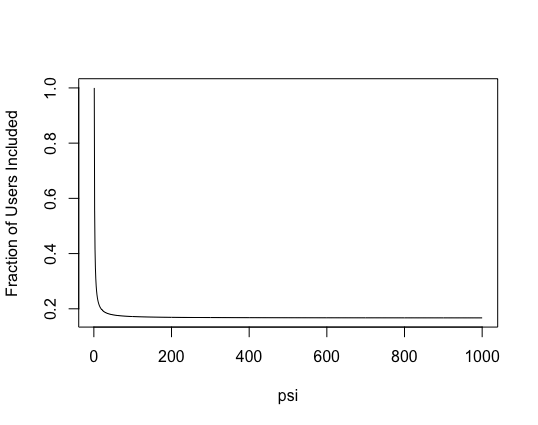
\includegraphics[width=10cm]{Fraction of users included.png}
  \caption{Fraction of users, $v$ vs. $\psi$}\label{fig:Fraction of users,v, vs. tildepsi}
 \end{figure}

$v \simeq \tilde{\psi}_t^{-2}$ as $\tilde{\psi} \rightarrow \infty$ with a $p$-value $<< 0.01$. This matches the generalized equation for BA models: $v = m^2k_t^{-2}$, where $m$ is the minimum number of connections any node in the model has (here $m = 1$) \citep{pastor2001epidemic}. This can then be manipulated to: $\tilde{\psi}_t \simeq v^{-1/2}$. 

This means that the probability of a random individual connected to a vaccinated node would be $p(v) = \sqrt{v}$. From there, $\langle \tilde{\psi} \rangle_t \simeq 2$, and $\langle \tilde{\psi}^2 \rangle_t \simeq 2 \ln(v^{-1/2})$, with $\tilde{\psi}_t = v^{-1/2} \rightarrow \infty$. This can be combined with equation \ref{v_c equation} to determine $v_c$, the critical fraction that needs to be vaccinated:
\begin{equation}
\label{reduced v_c} 
    v_c \simeq \exp{(-2/\lambda)}
\end{equation}

This equation has  been applied to examples such as viruses in the internet \citep{kephart1993computers}, STI transmission \citep{anderson1992infectious,lloyd2001viruses}, and other epidemics \citep{diekmann2000mathematical}. 

By this point, it should come as no surprise that "vaccinated" and "fact-checked" are interchangeable for the context of this thesis. Equation \ref{reduced v_c} can be easily adapted for a variety of scenarios. It can be used with an average $\langle \lambda \rangle$ for all tweets to determine the threshold of tweets/users to fact-check; in a situation like conspiracies about forest fires being spread by Antifa \citep{robinson2020oregon}, $\lambda_i$ can be calculated for that particular topic and $v_c$ can be used to calculate the number of tweets that must be fact checked. Much like it's unnecessary to vaccinate every node during an epidemic in order for the disease to die out, it is similarly unnecessary to fact check all possible tweets in order for a thread of misinformation to die out. 

Indeed, this meets the requirement posed at the beginning of this subsection: a relationship between $v_c$ and $j$ is created, since $\lambda = \frac{a}{j}$.


\subsubsection{$v_c$ Overlap}
On this note, there is likely to be heavy overlap in the individuals who would fall into $v_c$. As Imran Ahmed noted in an NPR interview in 2021, 29 million people follow only 10 individuals who spread anti-vaccine content \cite{npr2021teachers,ahmed2020antivaxx}. In October 2020, The National Vaccine Information Center (NVIC), the leader in anti-vaccine content, held a conference that featured many prominent anti-vaccine speakers, such as Robert F. Kennedy Jr. (1.3 million followers) and Joseph Mercola (3.6 million followers) -- it should be noted that Kennedy Jr. has since been removed from Instagram for spreading anti-vaccine conspiracy theories \cite{robinson2021instagram}. It should also be noted that Mercola -- and several other prominent alternative medicine proponents -- have made millions selling alternative medicines while attacking traditional medicine \cite{satija2019major}. This is all in line with the discussion earlier about $u^*$ and partisan overlap: users who subscribe to the beliefs of $u^*$ are likely to subscribe to the beliefs of the other similar users with high $|\psi|$ values. There is likely to be high overlap in the set of users who follow Kennedy Jr., Mercola, and the other speakers at this particular conference. If social media had removed all of the key speakers, it would have -- at least temporarily -- severely damaged the anti-vaccine misinformation network. 


\subsubsection{Summary and Metric}

Therefore, let:
\begin{equation}
\label{mu_4 and mu_5}
\begin{split}
    \mu_4 = v_{c,t} & = \exp(-2/\lambda_{t}) \\
    \mu_5 = v_{c,i} & = \exp(-2/\lambda_{i}) \\
    \mu_6 = v_{c,N} & = \exp(-2/\langle \lambda \rangle)
\end{split}
\end{equation}

$\mu_4$ should be interpreted primarily as a sense of urgency at the individual tweet level, while $\mu_5$ is at the topic level. While they are not the only metric connected to the $a \ln j$ equation, they \textit{do} contain $\lambda$ without a knowledge of $\langle \lambda \rangle$, the $|\psi|$ values of the members, or any analysis of the content. It is, effectively, self-contained. This is invaluable in meeting the requirement proposed at the beginning of this subsection: the ability to create a more apples-to-apples comparison between tweets and topics. 

Finally, $\mu_6$ uses $\langle \lambda \rangle$ to provide an overall health metric of the network. This can be treated as a key performance indicator (KPI) for the fact-checking team: if this process is being successfully utilized $\mu_6$ should remain static or decrease; if $\mu_6$ increases or approaches 1, then the network is becoming ungovernable. Either more checkers must be hired or more draconian rules must be implemented.

\subsection{Algorithm}
Combining all of these metrics and steps together provide the following algorithm/pseudo-code. Let "Every time step" be a partitioned unit, such that one fact checker can check one tweet in that step. If there are seven fact-checkers working simultaneously, then seven tweets can be checked ine one time step.

Let $F$ be a subset of $T$, such that $F$ is the set of tweets that will be fact checked at this point in time.

Let $V$ be a subset of $T$, such that $V$ are the tweets that have been fact-checked already and have been removed if false - in other words, vaccinated nodes.

\begin{algorithm}
\label{Ranking System Algorithm}
	\caption{Ranking System}
	\begin{algorithmic}[1]
		\For {Every time step}
		\State Remove all members of $V$ from $F$
		\If {$u$ in the list of white-listed users}
		\State Add $t$ to set $V$
		\State Remove $t$ from set $F$
		\EndIf
		\State Perform natural log regression for the cumulative sum of retweets of each tweet
		\State Remove all $t$ from $F$ where the coefficient for $a\ln x$ is NULL
		\State Calculate $\mu_1$ for each available $t \in F$
		(Eq.: \ref{mu_1 equation})
		\State Calculate word pair $EWMA$ and $EWMVar$ for all tweets in $F$ (Eq.: \ref{Finch Equations})
		\If {any word pair in $t$ is in $EWMA$ and $EWMVar$}
		\State Add $t$ to set $I$ for that word pair
		\EndIf
		\State Calculate $\mu_2$ for each available $t \in F$ (Eq.: \ref{mu_2 equation})
		\State Calculate $\tilde{\psi}$ for each user (Eq.: \ref{psi immunized})
		\State Calculate $\mu_3$ (Eq.: \ref{mu_3 equation})
		\State Calculate $\mu_4$ for $F$ (Eq.: \ref{mu_4 and mu_5})
		\If {$t \in I$}
		\State Calculate $\mu_5$ for $I$ (Eq.: \ref{mu_4 and mu_5})
		\EndIf
		\State Calculate unique value $\zeta$ for each $t$ (Eq.: \ref{zeta function})
		\State Rank the tweets by $\zeta$ value (Eq.: \ref{ranking equation})
		\While{In current time step}
		\For{All tweets in $F$}
		\State Fact check $t^*$ 
		\State Add $t^*$ to $V$
		\State Remove $t^*$ from $F$
		\State $t^* \xleftarrow[]{} t^{*-1}$
		\EndFor
		\EndWhile
		\EndFor
	\end{algorithmic} 
\end{algorithm} 
\newpage
\subsection{Summary: The Circuit Breaker}
A reasonable person may argue that $t_2$ from the ordered set may actually be more important to fact check than $t_1$, as there are multiple strains of misinformation covering multiple topics every day.  For example, in late 2020, there was a wide spread in misinformation surrounding the COVID-19 vaccine \cite{mills2020covid,bagherpour2020covid}. Concurrently, false claims of fraud in the 2020 U.S. election \cite{dean2020facebook} spread before being replaced with plans for a violent insurrection on January 6th at the U.S. Capitol \cite{fandos2021trump,Levenson2021capitol}. Each of these topics is dangerous; each stands to have a high cost in human life and suffering. Reasonable people could make cogent arguments about one thread of misinformation being more or less dangerous than the other. However, fact checkers can only check so much and only check so quickly, so any ranking will leave room for criticism.

Because of that, this thesis proposes that the five metrics (and their corresponding weights) be used not only to rank the content that needs to be fact checked, but also as a circuit breaker. Content where $\zeta$ is greater than a particular threshold, $\zeta_t$ can be quarantined pending fact-checking. This is not a radical proposal: circuit-breakers are used in global financial markets during times of extreme volatility \cite{wang2019microstructure,schwert1990stock} and can promote market-wide stability by "preventing the spread of poor market quality" \cite{brugler2014single,schneider2020stock}. Indeed, this proposal has already generated discussion by experts \cite{goodman2020digital,simpson2020fighting} and Facebook has expressed interest in adding "speed bumps" \cite{bond2020circuit}.

Furthermore, this proposed solution resolves all of the issues in section \ref{sec: currently implemented solutions}: it is scaleable, it is not a black-box solution, it does not limit freedom of speech unnecessarily, yet it also will actively remove dangerous content from the platforms according to how dangerous it is.

\section{Implementation and Experimentation}
In order to test this proposed ranking solution, three data sets are used. The first set, \textit{Twitter15}, is the set that has been used in many other papers on this topic. It is therefore important to include for the sake of comparability.

The second set was created with generous help from Twitter, and will be referred to as \textit{Twitter21} to differentiate it. 

Finally, the third set will be a stochastic set. Because of the amount of information required, most Twitter sets are quite small. To rectify this, a randomly generated model will be used as a final test for this solution. That set will be called \textit{Stochastic21}.


\subsection{Twitter15}
 The publicly available \textit{Twitter15} set, generated as part of the work of Ma et al (2016), has been used in multiple articles and theses \citep{liu2018early,ma2017detect,ma2016detecting,khoo2020interpretable,liu2019early,huang2019deep}. This thesis will look at Liu's adjusted \textit{Twitter18} set, which makes a few cleaning adjustments: namely tweets labeled "unverified" have been removed, tweets that are no longer accessible have been removed from the set, and 353 true and 327 fake stories have been added to supplement the removed tweets \citep{liu2019early}. 
 
 However, the \textit{Twitter15} (and by extension the adjusted \textit{Twitter18}) set has four flaws that are not discussed in surrounding literature. 
 
\subsubsection{Caveats}
First, it sets all tweets to $\tau \in \{0,1\}$, which is not a realistic depiction of the set of tweets being evaluated, save those that are \textit{a priori analytic}, \textit{a priori synthetic}, or \textit{a posteriori analytic} (discussed in \ref{truthvalue appendix}). Even if all the tweets in the set fall into those three groups -- in which case the binary $\tau$ is reasonable -- the sample set would then not realistically depict the population of all tweets. Therefore, their true/false metrics will be referred to as $\tau'$, a binary operator illustrating if a fact-checker has flagged this tweet for removal.

Second, those truth values $\tau'$ are highly problematic. A great deal of content is marked as "non-verified rumor" or "false" that is not actually untrue. For example, the most retweeted tweet in the first 24 hours in this set and has $\tau' = 0$ is this tweet from ESPN (fig. \ref{fig:ESPN Tweet, April 20, 2016}). Arguably, this counts as \textit{synthetic a posteriori} knowledge, but the content is not intentionally misleading or untrue. 
 \begin{figure}[h!]
    \centering
    
\includegraphics[width=9cm]{espn Mcgregor tweet.png}
    \caption{ESPN Tweet, April 20, 2016 \cite{espn2016tweet}}
    \label{fig:ESPN Tweet, April 20, 2016}
\end{figure}

The same is true of the second most retweeted "false" tweet in the set from the BBC (fig. \ref{fig:BBC Breaking Tweet, Jan 18, 2016}).
\begin{figure}[h!]
    \centering
    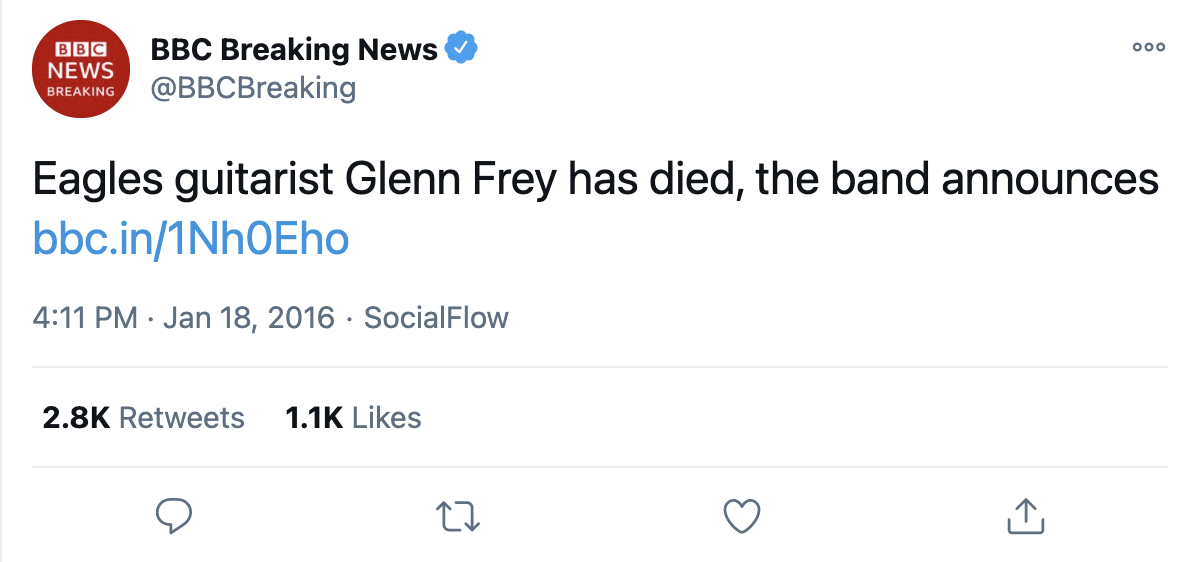
\includegraphics[width=9cm]{BBC Eagles.png}
    \caption{BBC Breaking Tweet, Jan 18, 2016 \cite{bbc2016tweet}}
    \label{fig:BBC Breaking Tweet, Jan 18, 2016}
\end{figure}
That tweet is also marked as a "rumor", even though it was not only true but from a reputable source. This data set does not differentiate between reputable (referred to as white-listed here in \ref{sec: white listing}) and disreputable sources, nor does it do any post-hoc validation. This makes the truth values for this set highly problematic, and makes all of the RNN analyses off of this set equally untrustworthy. This thesis therefore discards the results of \citep{liu2018early,ma2017detect,ma2016detecting,khoo2020interpretable,liu2019early,huang2019deep} in terms of classification of fake news and rejects the $\tau'$ values provided by this set.

Third, it has a disproportionately high number of users who are verified ($v = 1$). Twitter's requirements for being a verified account require follower count in the top 0.1\% of active accounts in a particular region or proof of being an important person off of twitter, such as being a professional artist/athlete, elected official, etc. \citep{twitter2020verified}; however, 1.4\% of the users in this set are verified. If verified is used as a quick stand-in for hub node, there are 14 times more hub nodes than would be expected in a random sample of twitter users. At the same time, there may be more verified users than \textit{necessary} hub nodes. Since the total number of verified users is 3,061 with 212,360 unverified in the \textit{Twitter15} data set, yet the Arapacio set proposed only 1,000 hub nodes out of a set of 50,000,000, it is likely that users who are \textit{necessary} hubs and users who are verified are not equivalent sets. Hub nodes are likely a subset of verified users. 

Fourth, it breaks down the retweet paths into ordered pairs $(u_i,j_i)$ with $u_i$ being the user retweeting and $j_i$ being a batched time interval which is correlated but not equal to the actual time the retweet was posted. In order to make their data set more RNN friendly, each retweet path was batched and partitioned, so that the length of entire time series for each retweet path is unique, but the distance between intervals is equal \citep{shu2017fake}. In other words, $j$ values are comparable across tweet paths, but are divorced from the actual time of posting.



 \subsubsection{User Data}
However, on the whole, this set matches much of the previous analysis. When plotting the $Y$ and $Z$ on a $\log_{10}$ scale (fig. \ref{fig:Twitter15 Follower}, fig. \ref{fig:Twitter15 Following}), the distribution is relatively normal and the power law (equation \ref{powerlaw}) holds true here:  $\gamma_{in} = 2.6$ and $\gamma_{out} = 1.62$. This is quite close to the $\gamma_{in}$ and the $\gamma_{out}$  from the Arapacio data set, 2.2 and 1.9 respectively.
 
 \begin{figure}[h]
\minipage{0.5\textwidth}
  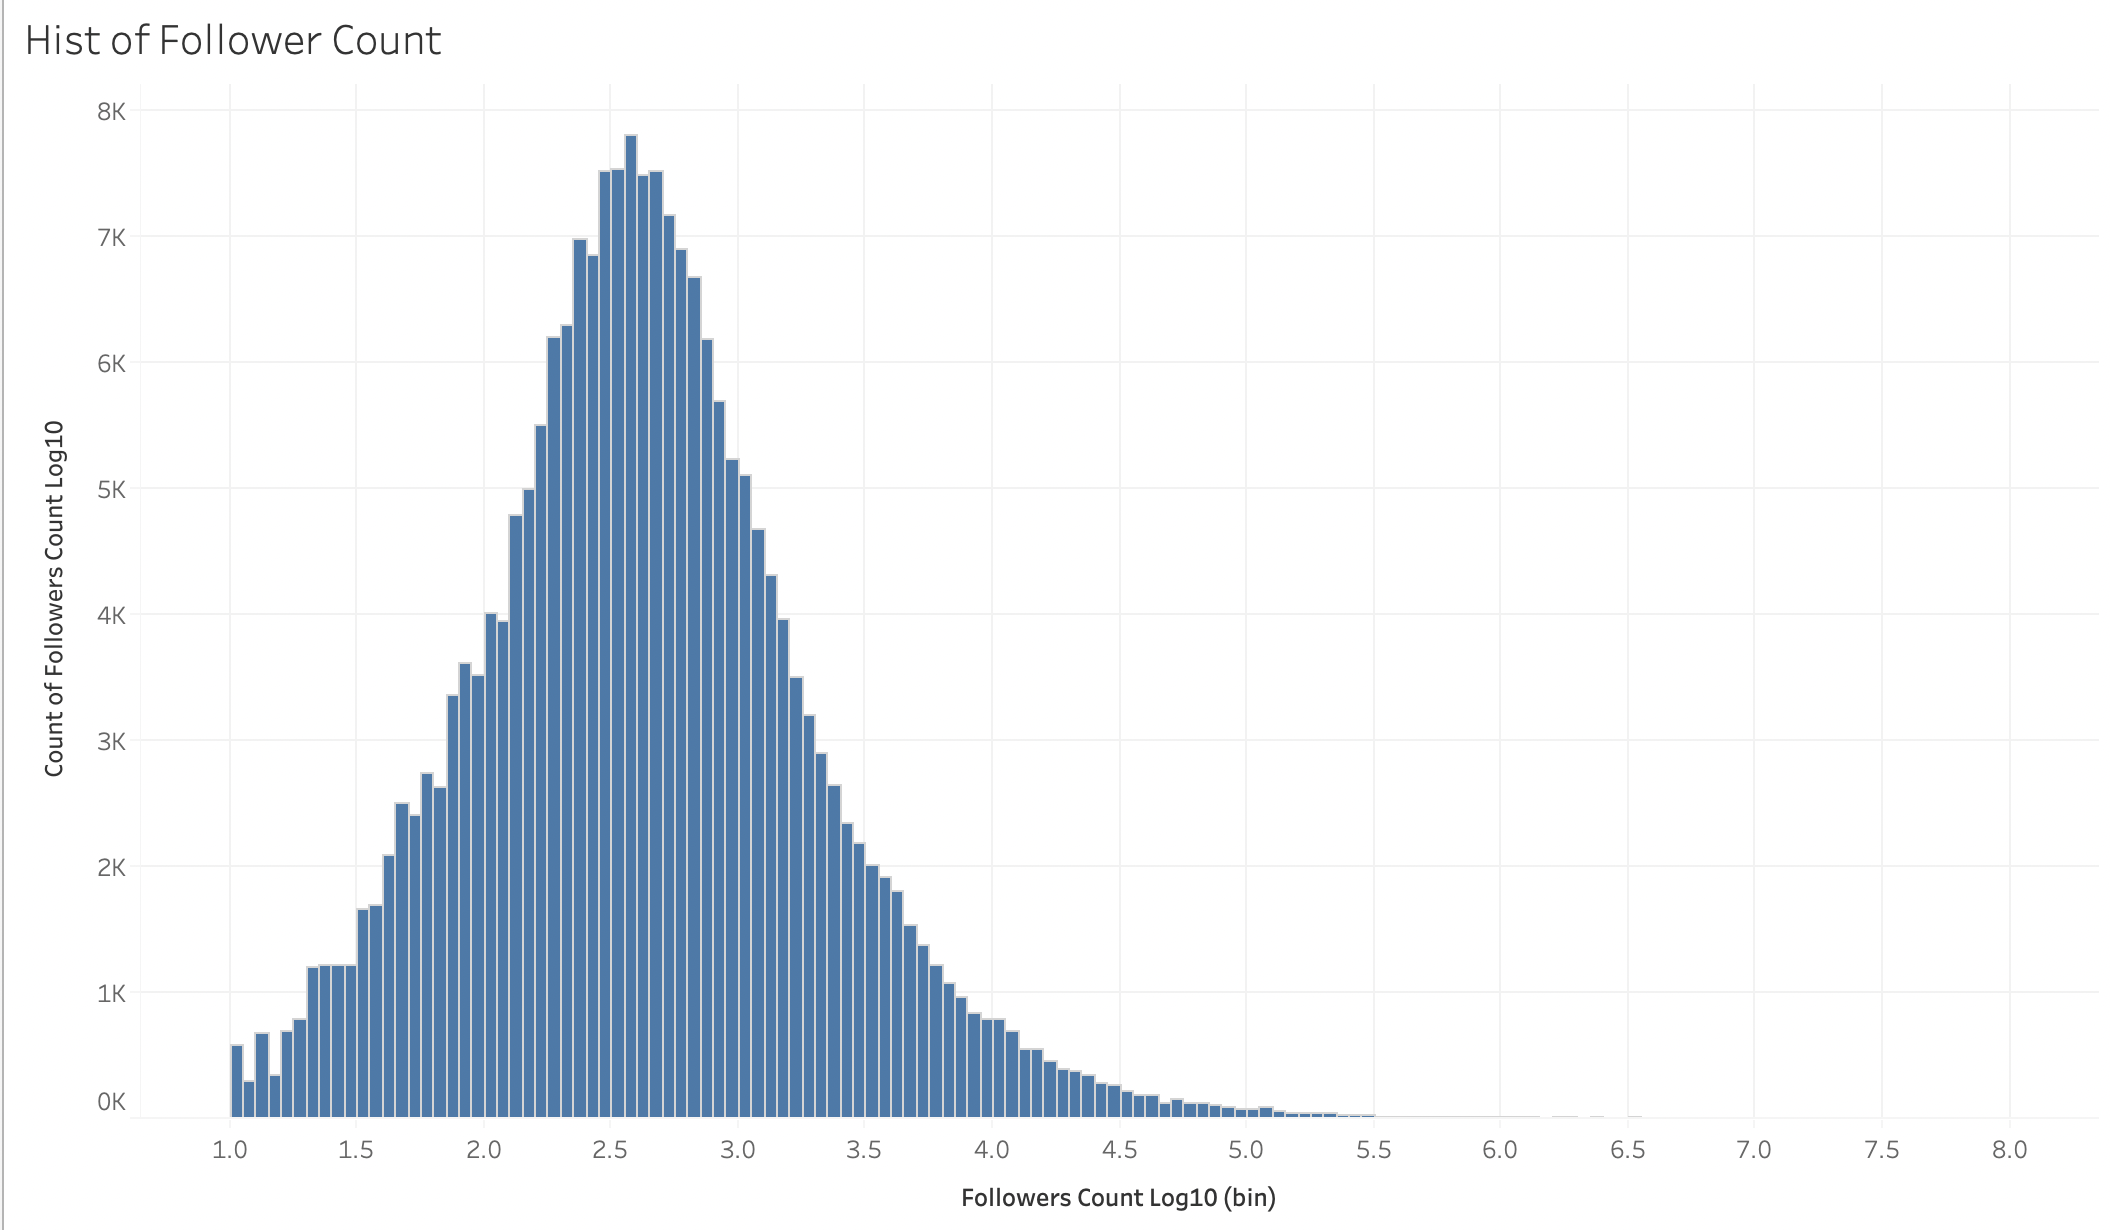
\includegraphics[width=\linewidth]{Twitter15 Follower Count.png}
  \caption{Follower Count, $|Z|$, for Twitter15 Set}\label{fig:Twitter15 Follower}
\endminipage\hfill
\minipage{0.5\textwidth}
  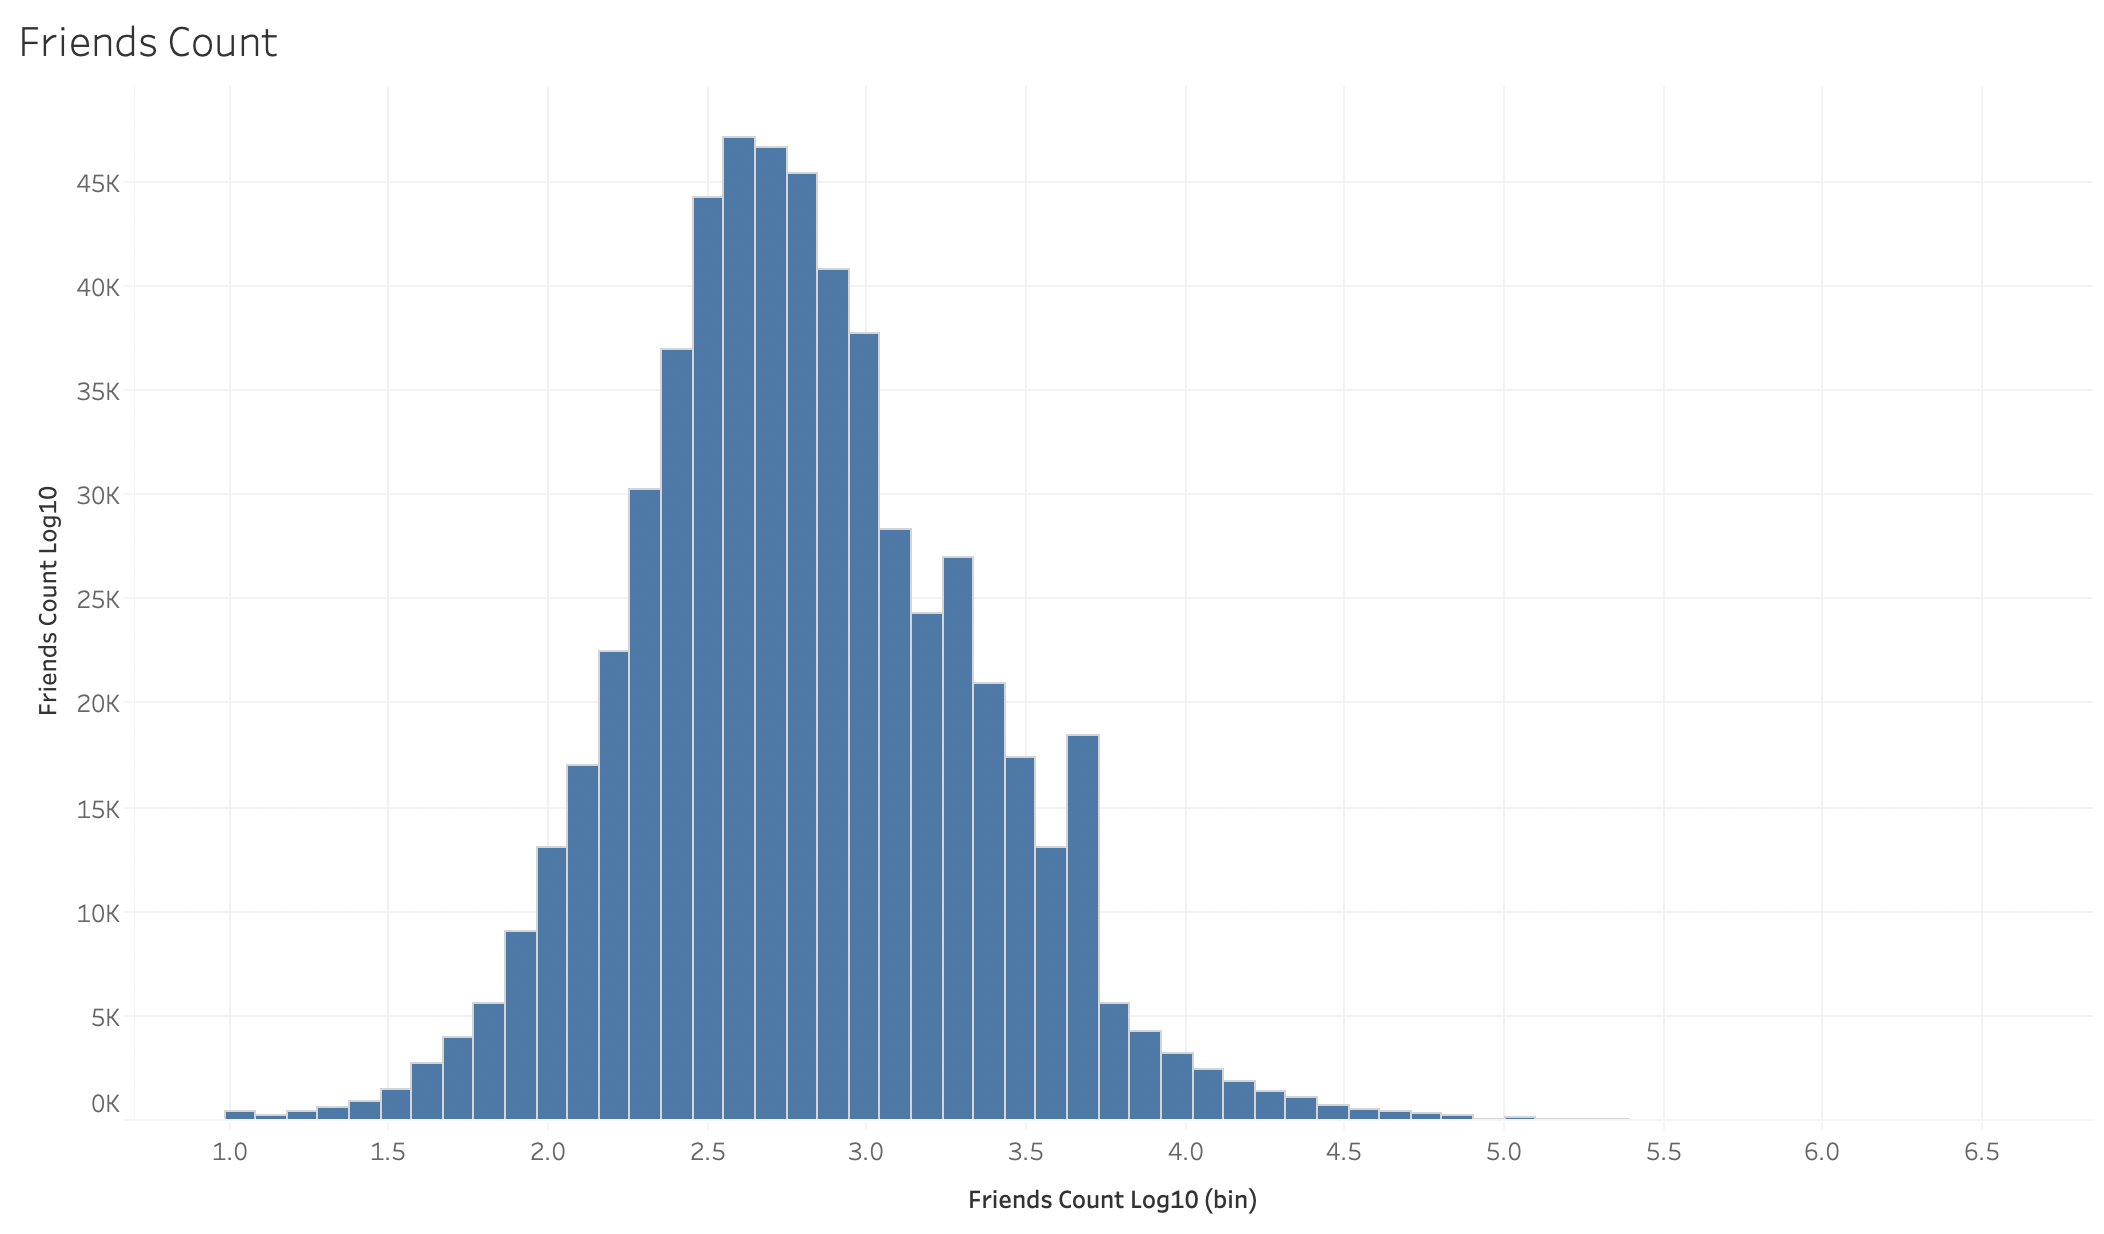
\includegraphics[width=\linewidth]{Twitter15 FriendsCount.png}
  \caption{Following Counts, $|Y|$, for Twitter15}\label{fig:Twitter15 Following}
\endminipage\hfill
\end{figure}



If the verified binary, $v \in \{0,1\}$, is a stand-in for hub nodes in this set, even though it is overly generous as discussed earlier, then non-hub nodes are close to the Arapacio numbers but hub nodes have an even greater $\frac{|Y|}{|Z|}$ than in the Arapacio set:
\[
\begin{split}
& \forall \ u_n, v_n  = 0:\langle |Y_n| \rangle \leq 400, \langle |Z_n| \rangle \leq 500, \langle  \frac{|Y_n|}{|Z_n|} \rangle \approx \frac{4}{5} \\ &\text{and} \\ & \forall \ u_n, v_n  = 1:\langle |Y_n| \rangle \leq 18,000, \langle |Z_n| \rangle \leq 1,300, \langle  \frac{|Y_n|}{|Z_n|} \rangle \approx 13.8
\end{split}
\]
\textit{Twitter15}'s 13.8 is clearly much greater than Arapacio's $\frac{7}{10}$; this could be due to the time the sample was collected as the Arapacio set was collected in 2009 and total user count has expanded since then. The \textit{Twitter15} set contains, for example, former President Barack Obama, whose account has over 110M followers. 

Regardless, this set meets the requirements of a scale free network, and therefore all previously analyzed equations, such as equations \ref{Ldotpartisan} and \ref{echo chamber by followers} will be applied here.

\subsubsection{Retweets}
The retweet data, as mentioned earlier, is a vector of ordered pairs of users and time intervals so that $ \exists \ \vec{r}:\{(u_1,z_1), \cdots, (u_n,z_n)\} \ \forall \ t \in T$.

The total number unique users retweeting each tweet in the set is illustrated in fig. \ref{fig:Unique Retweeters}, and has the following properties as described in table \ref{Retweet Unique User Counts}:
\begin{figure}[h]
 \centering
  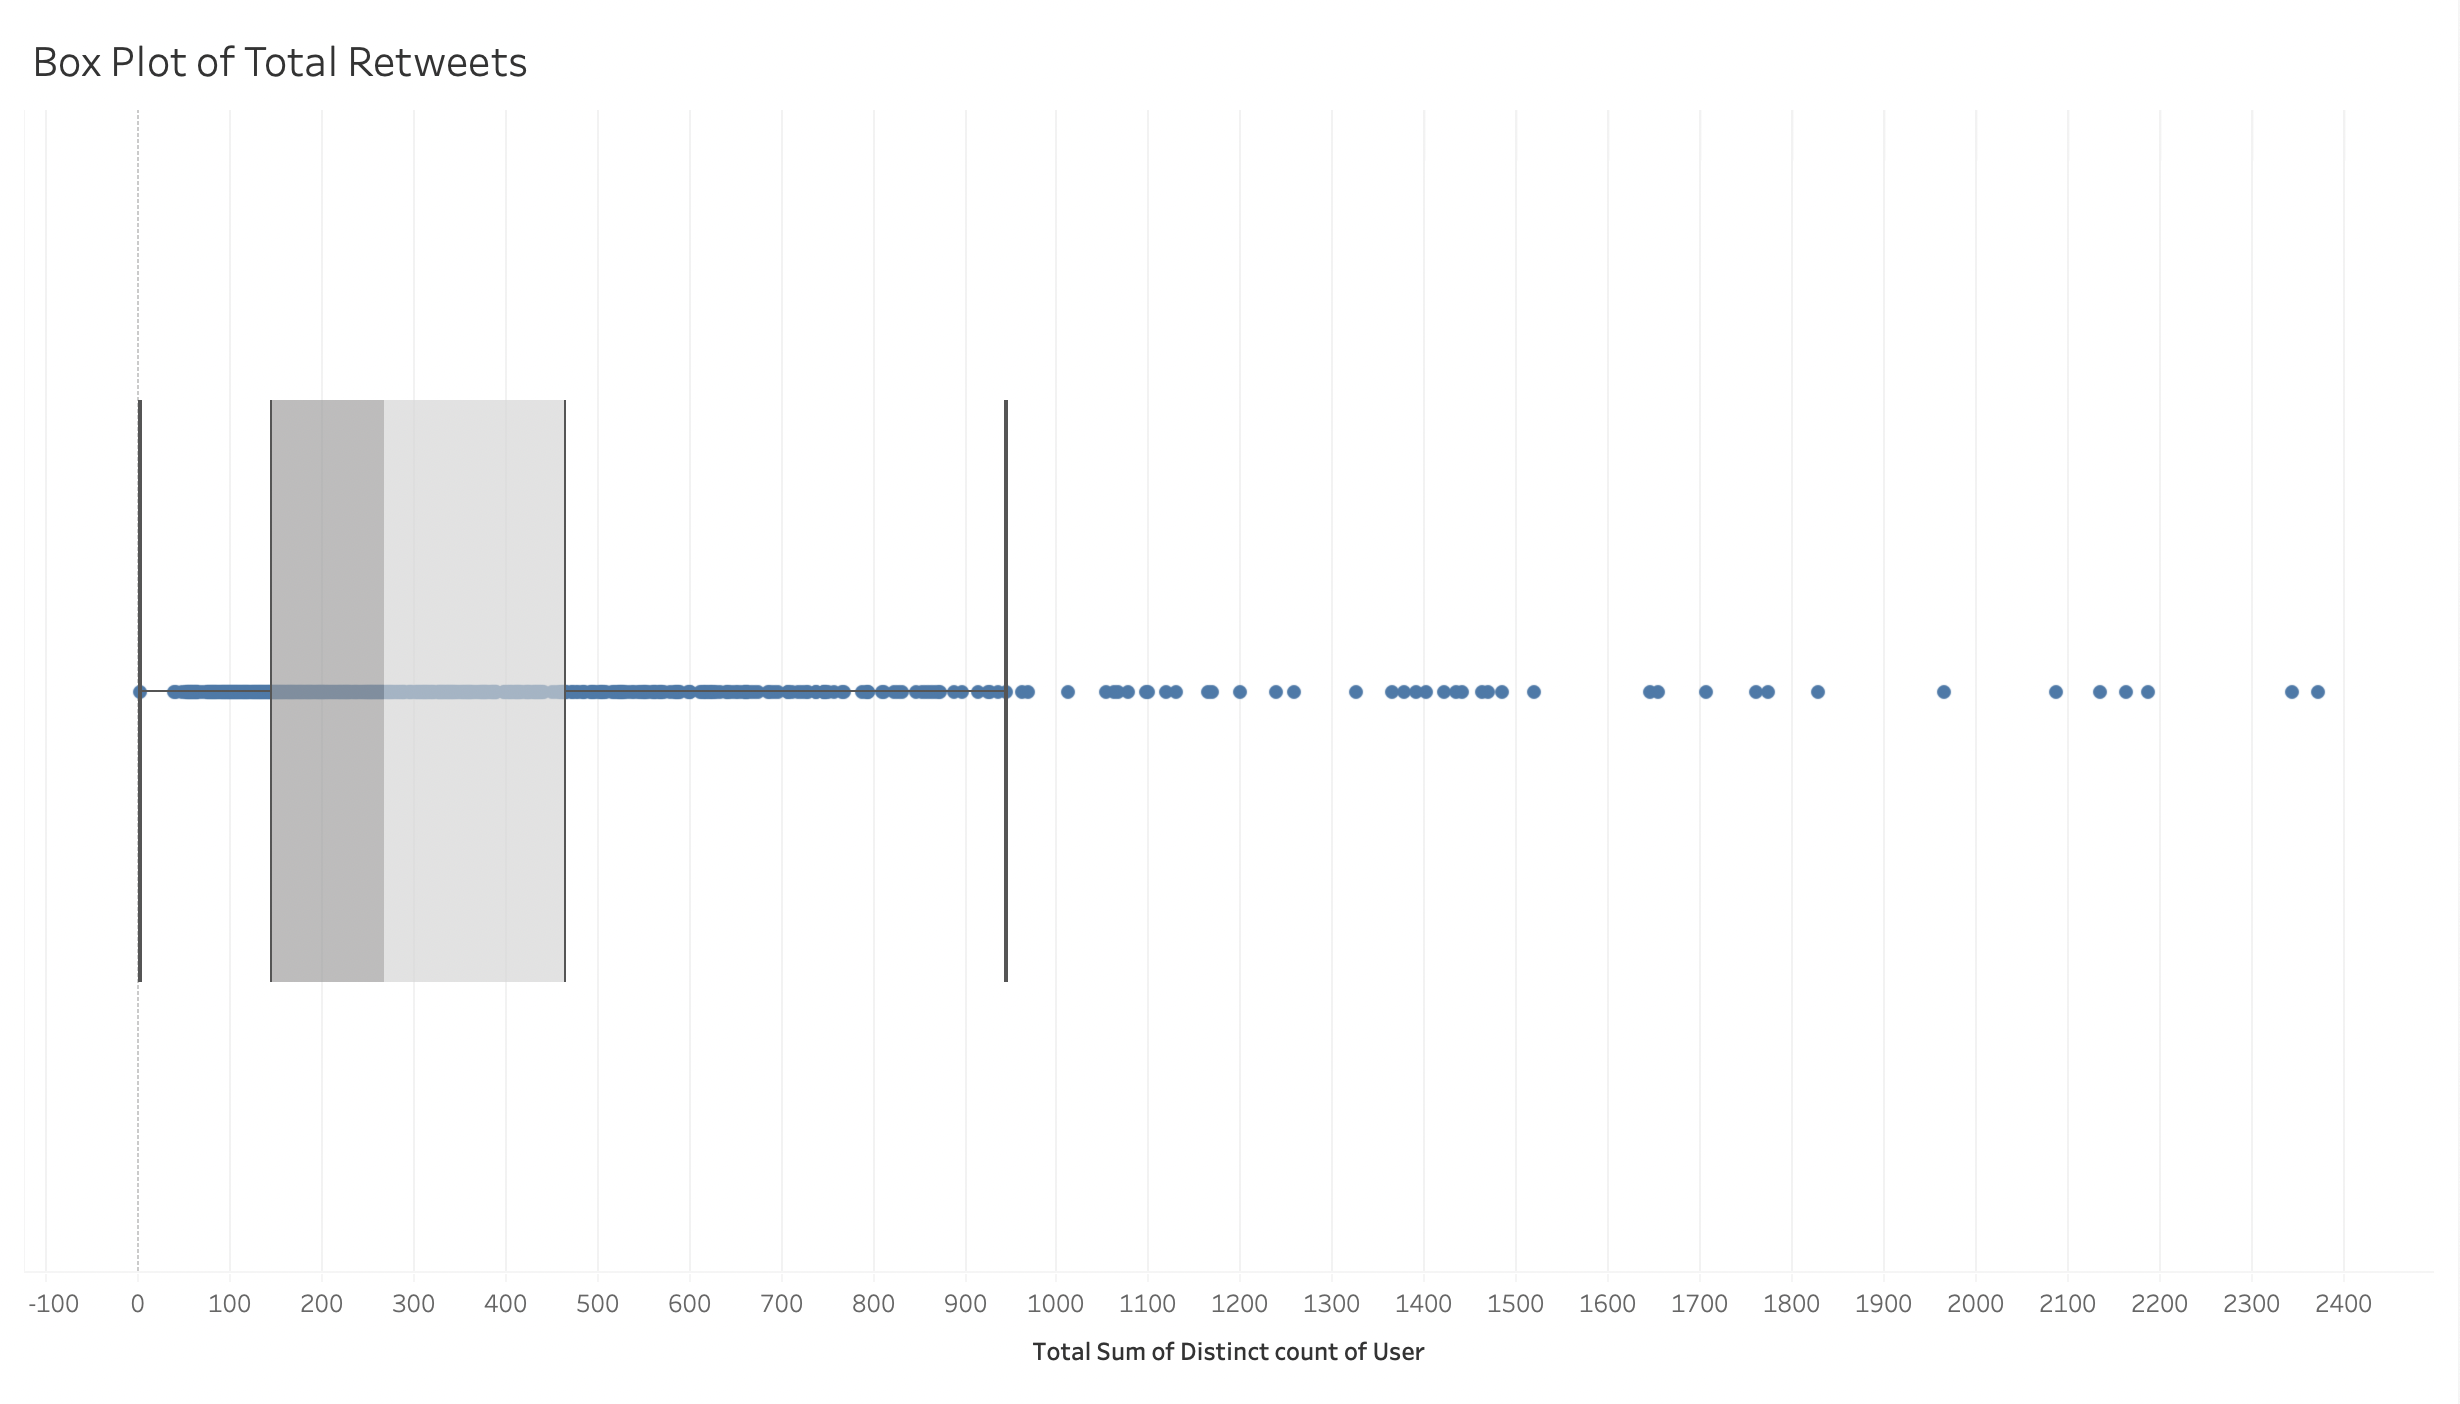
\includegraphics[width=12cm,height=5cm]{Retweet Box Plot.png}
  \caption{Box Plot of Unique Users Retweeting Each Tweet in the Data Set}\label{fig:Unique Retweeters}
 \end{figure}
 
\begin{table}[h]
\centering
\begin{tabular}{ |p{3cm}|p{3cm}|  }
\hline
\multicolumn{2}{|c|}{Retweet Unique User Counts} \\
\hline
Lower Whisker & 2\\
Lower Hinge & 146 \\
Median & 267.5 \\
Upper Hinge & 465.5 \\
Upper Whisker & 945 \\
\hline
\end{tabular}
\caption{Retweet Unique User Counts}
\label{Retweet Unique User Counts}
\end{table}

 
A graph of the running total of the number of unique users who have retweeted a particular tweet in figure \ref{fig:Users CumSum/Time} shows that the relationship is clearly logarithmic, which aligns with this thesis's previous analysis and proposals. The graph is set to a maximum $z = 24$ as one of the goals of this thesis is to rapidly identify tweets that need to be flagged for verification.
\begin{figure}[h!]
 \centering
  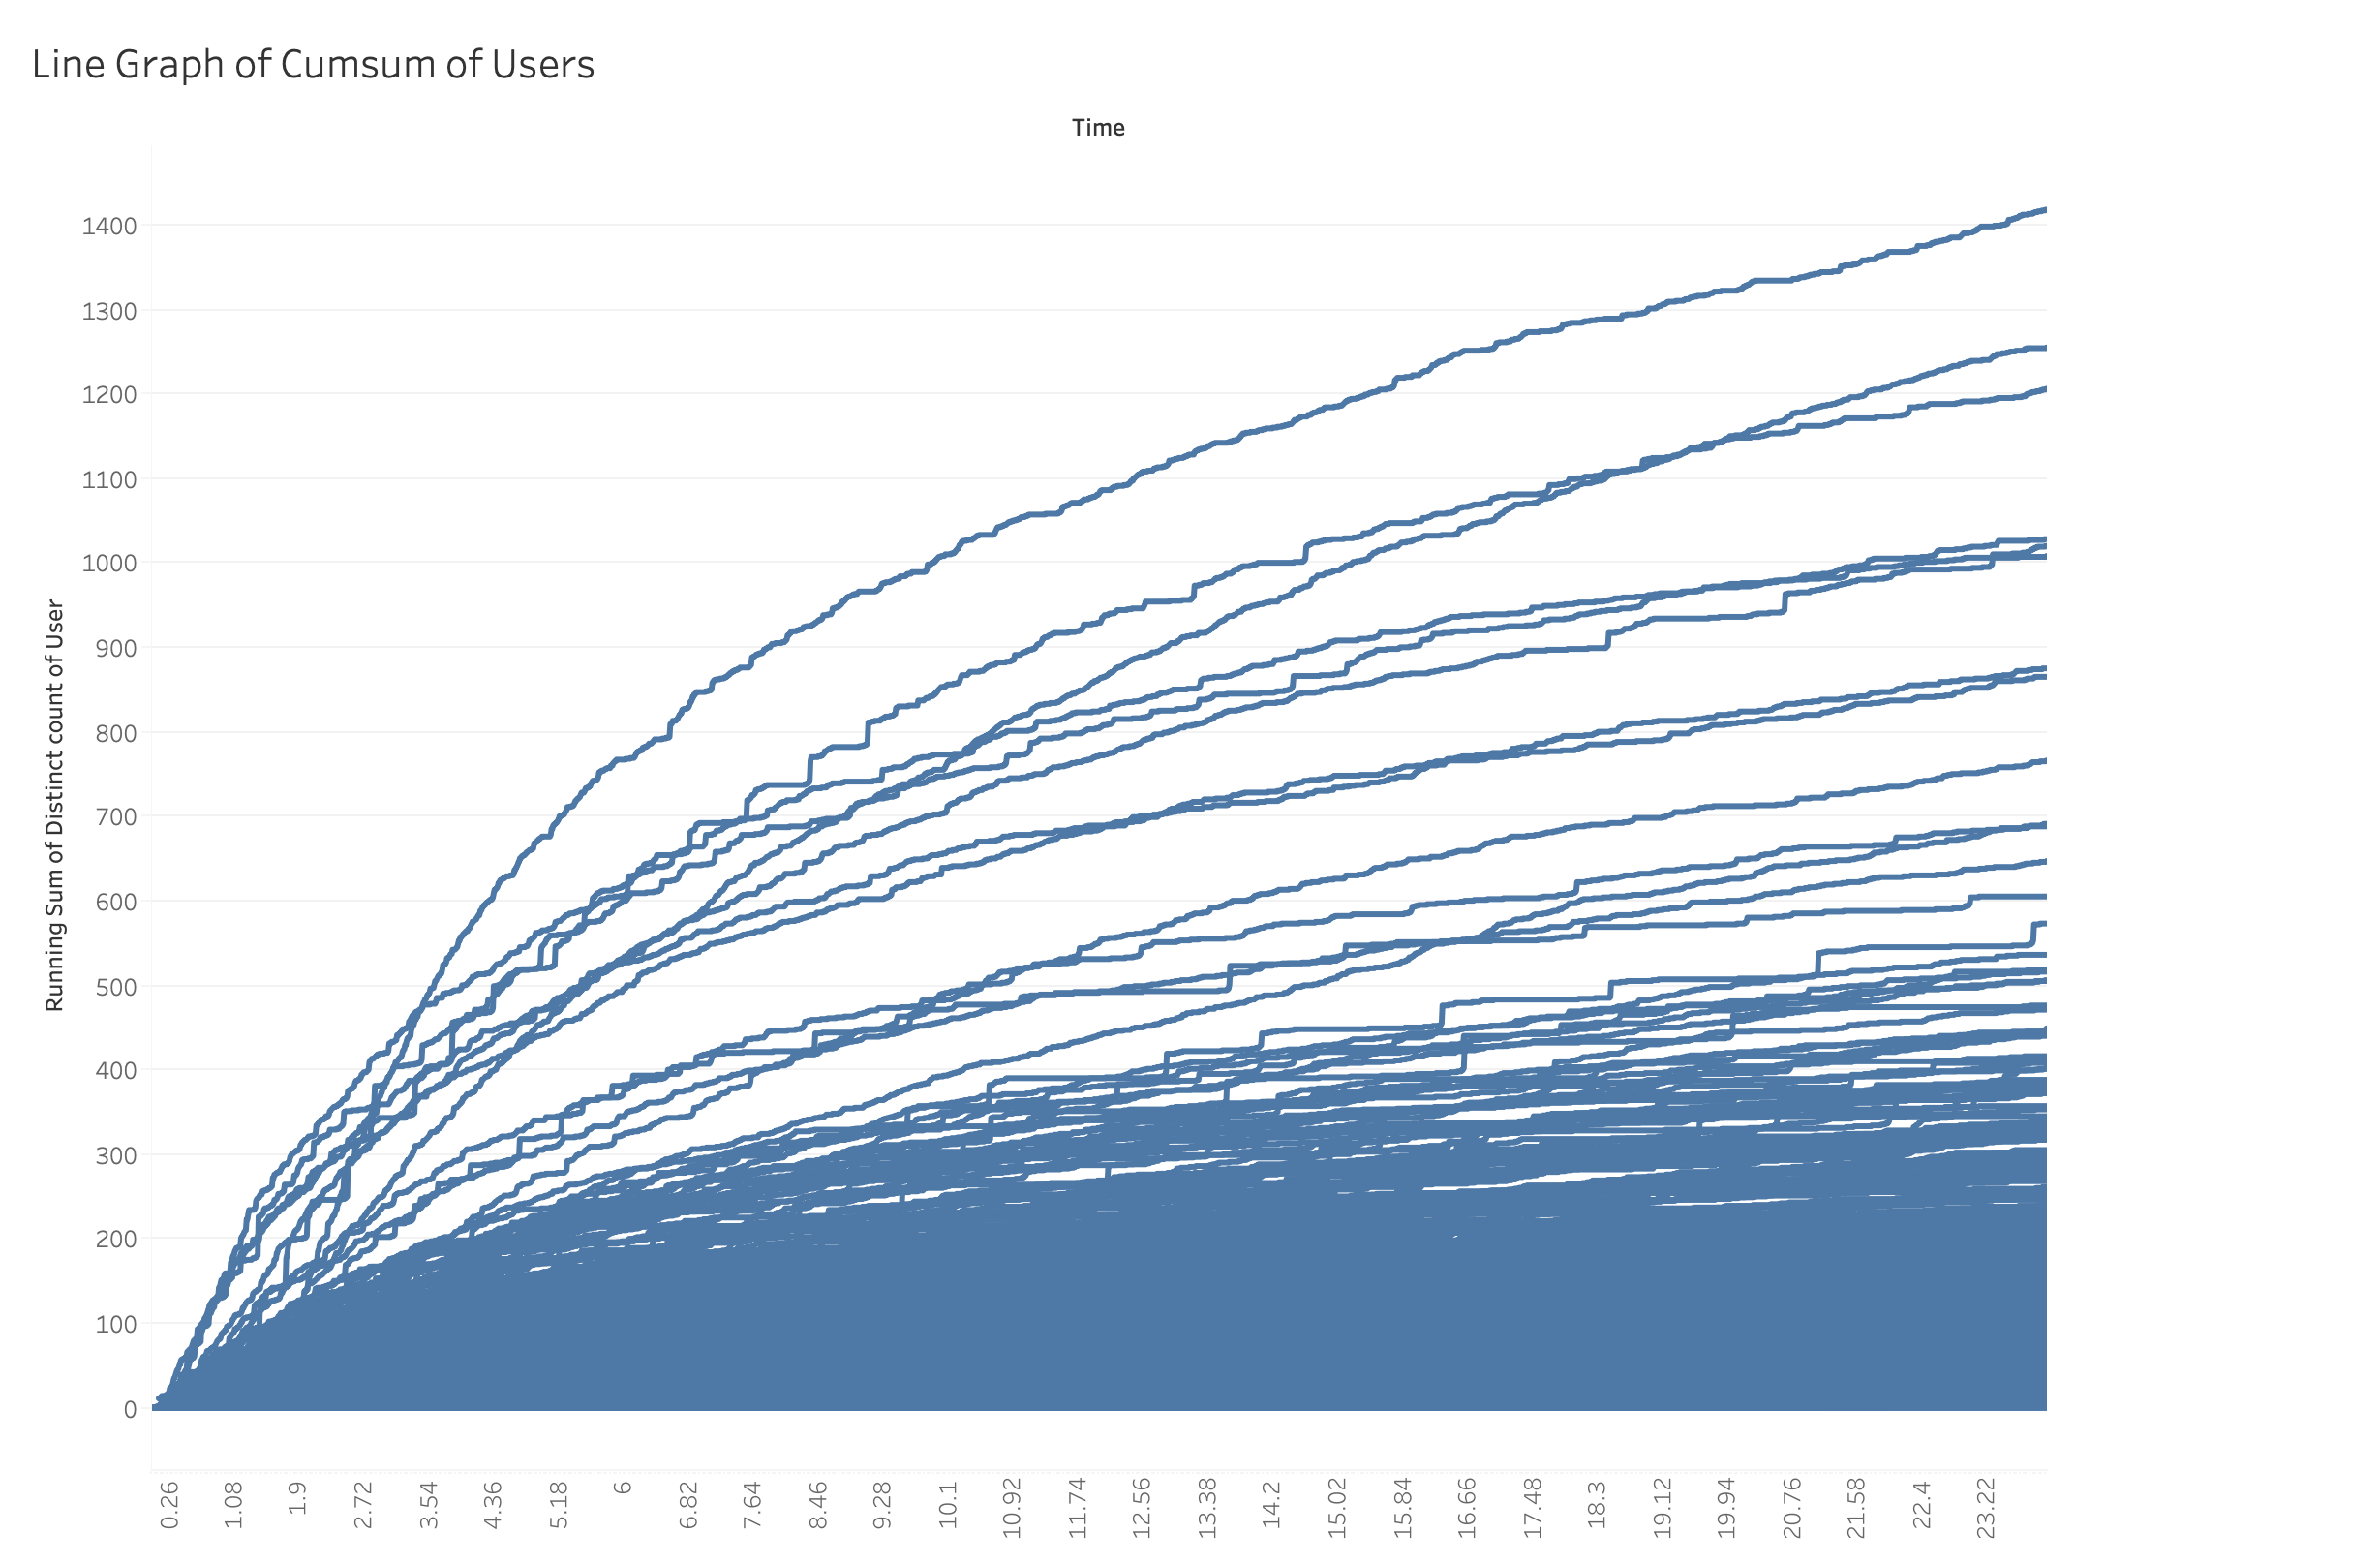
\includegraphics[width=12cm]{Linegraph cumsum users.png}
  \caption{Line Graph of Cumulative Sum of Retweeters over Time}\label{fig:Users CumSum/Time}
 \end{figure}

With simple regression to calculate the cumulative number of unique users retweeting a tweet to an $a\ln(j)$ equation with an intercept of zero (the intercept is manually forced to 0 as no tweet has $\geq 1$ retweet when time is 0), the number of the 680 tweets that fell into each statistical relevancy set is in the table \ref{Natural Log Fit}. The N/A values come from tweets that were insufficiently retweeted (1 or fewer retweets).   
\begin{table}[h!]
\centering
\begin{tabular}{ |p{3cm}|p{3cm}|  }
\hline
\multicolumn{2}{|c|}{$p$ value for $a\ln(j)$} \\
\hline
$p < 0.05$  & 654\\
$N/A$ & 18 \\
$ p \geq 0.05$ & 8 \\
\hline
\end{tabular}
\caption{$a\ln(z)$ fit}
\label{Natural Log Fit}
\end{table}

For an average tweet, the cumulative number of users at can be described by the equation $f(j)=85.8\ln(j)$, which has a $p$-value $<< 0.05$. 

It is also interesting to note the number of tweets with an $a > 85.8$ as seen in table \ref{a > 85.58}. Slightly less than 10\% of all tweets tracked showed a higher $a$ value than the average tweet.
\begin{table}[h!]
\centering
\begin{tabular}{ |p{3cm}|p{3cm}|  }
\hline
\multicolumn{2}{|c|}{Number of retweet paths with $a$ value relative to $\langle a \rangle$} \\
\hline
$a > 85.8$  & 67\\
$N/A$ & 18 \\
$ a \leq 85.8$ & 595 \\
\hline
\end{tabular}
\caption{Number of retweet paths with $a$ value relative to $\langle a \rangle$}
\label{a > 85.58}
\end{table}


For this data set, let $\langle \rho_{\Delta} \rangle = 0.5$. Much of the content in this set is non-partisan in nature, such as the ESPN and BBC tweets shared earlier. This adjustment changes implies that $\langle \tilde{\psi} \rangle = \langle \psi \rangle$ for this set, as there is no partisan driven immunity (or susceptibility) in this set. This also allows for 
$\left(\frac{1-\rho_{\Delta}}{1-\langle\rho_{\Delta}\rangle}\right)$ in equation \ref{Pdotpartisan} to cancel out. Both of these are appropriate -- it is unlikely that an individuals political beliefs will shape their beliefs on whether or not Connor McGregor won a fight on a particular day. 

\subsubsection{Experimentation}
\label{sec: Twitter15 Experimentation}
Since this thesis proposes a ranking system, and this dataset is batch based, let it be proposed that a fact-checker can check 1 tweet per $j$ interval, which means that this checker can check 24 total tweets during the allotted time period.

Let it also be set that at the point the fact checking occurs, that path is declared vaccinated - regardless of $\mu$ values, there is no need to check that thread again. It has either been removed if determined false or it has been white-listed if true.

Since no weights have been determined yet for each metric, the metrics here have been minmax scaled such that each $\mu$ value is between 0 and 1: 
\[
\forall \ \mu \in \mathcal{M} \  \exists \ \mu' := \frac{\mu - \min(\mu)}{\max(\mu) - \min(\mu)} 
\]
This will allow each $\mu$ value to be equally valuable.

The following reputable news organizations were marked as white-listed: The Wall Street Journal, CNN, CNN International, CNN Breaking, BBC, BBCWorld, BBC Breaking, New York Times, ESPN, The Economist, Reuters, The Washington Post, Time, ABC, The AP, NBC Breaking News, CBS News.

The Onion, a satirical news site was also white-listed. Even though it posted tweets like fig. \ref{fig:The Onion Tweet, Jan 29, 2016}, which could be interpreted as "fake news" if someone believed it at face value, they make no pretenses about being a real news organization, and should not be included in this study as the fall under the category of sarcasm and irony discussed in the section on hyperbole, sarcasm, and irony (See: \ref{hyperbole}). By this same token, Mashable, Rolling Stone, E! News, and MTV were also removed as they serve primarily for entertainment and not news purposes.
\begin{figure}[h]
    \centering
    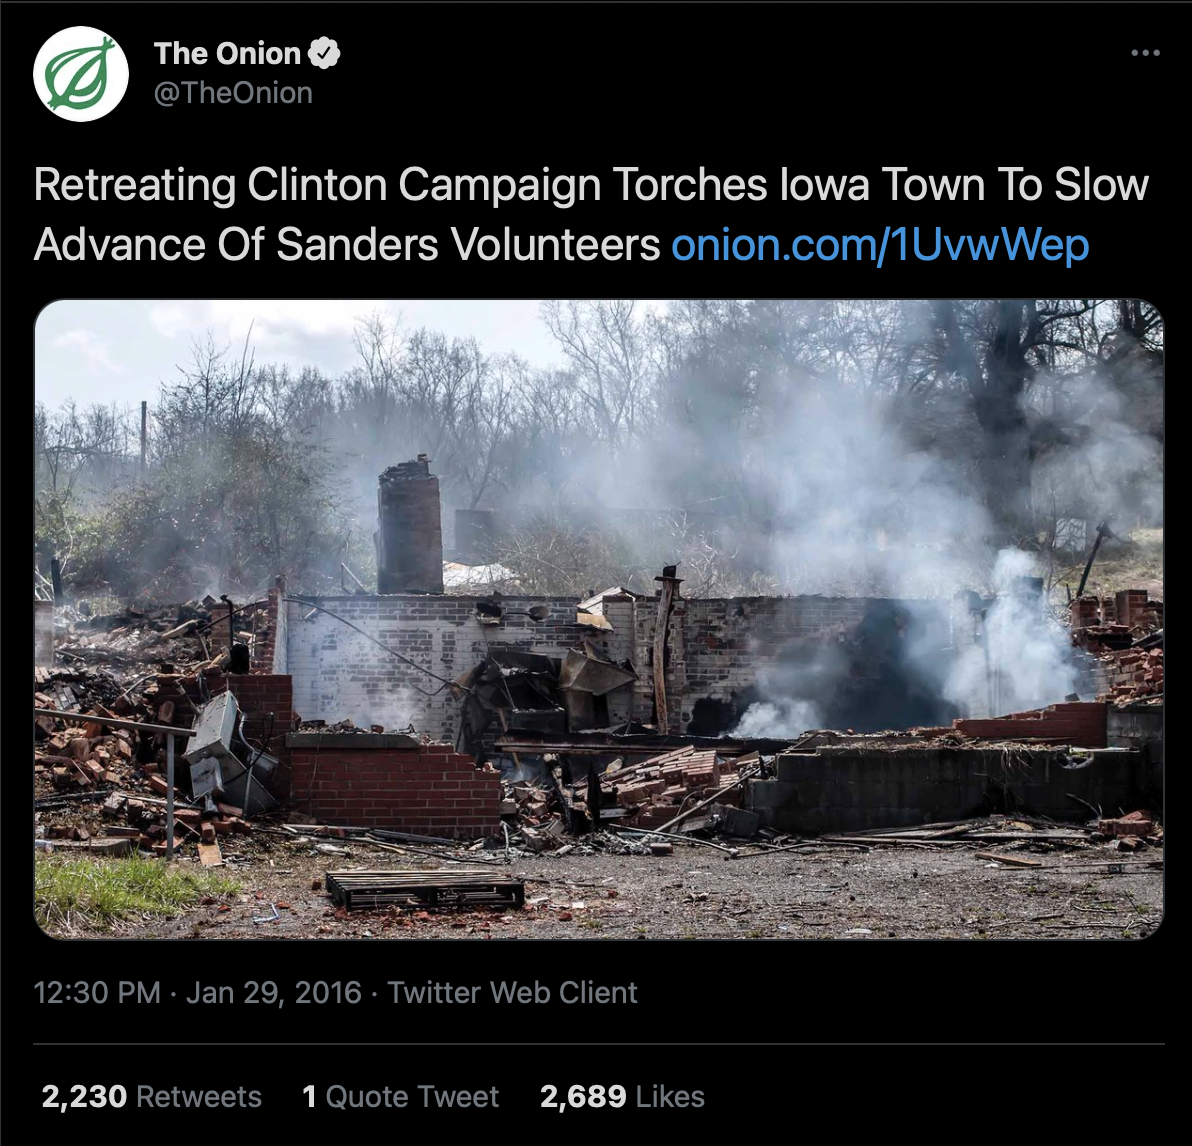
\includegraphics[width=8cm]{Onion Tweet.png}
    \caption{The Onion Tweet, Jan 29, 2016 \cite{onion2016tweet}}
    \label{fig:The Onion Tweet, Jan 29, 2016}
\end{figure}

The Obama White House official White House account was removed from this set, as their tweets were non-controversial in nature. On the other hand, The Huffington Post and Fox News were both left in this set.

Results for $\mu_1$:
\begin{figure}[h]
    \centering
    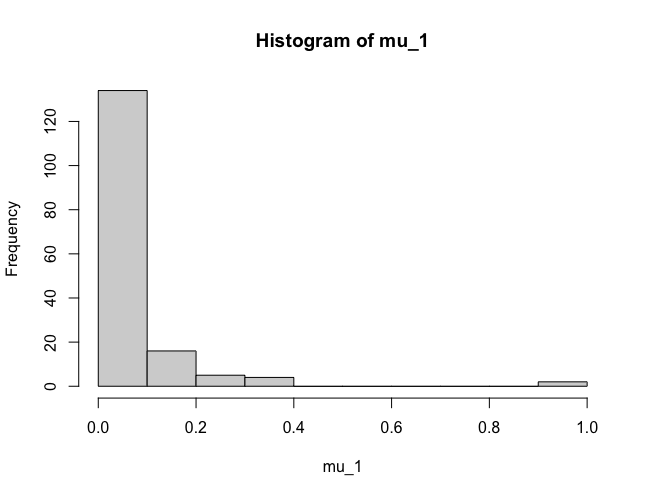
\includegraphics[width=8cm]{Histogram of mu_1 twitter15.png}
    \caption{Histogram of $\mu_1$ values for first time period for \textit{Twitter18}}
    \label{fig:Hist mu_1 Twitter18}
\end{figure}
The majority of the users here had relatively few followers (as illustrated in the user analysis earlier). 

Results for $\mu_2$:
These are the top 10 bigrams from the dataset and their corresponding counts. URLs were removed as well as words that were all non-alpha numeric. The \# was left in, as this is a relevant character for Twitter. This analysis was performed with NLTK tokenizer and counter:

\begin{table}[h]
    \centering
    \begin{tabular}{|p{4cm}|p{2cm}|}
    \hline
         Paul, Walker & 42 \\
         War, Memorial & 29 \\
         Paul, Walkers & 24 \\
         Soldier, Shot & 21 \\
         Malaysia, Airlines & 16 \\
         Died, Paul & 16 \\
         Breaking, News & 14 \\
         National, War & 14 \\
         Darren, Wilson & 14 \\
         Iphone, 6 & 13 \\
    \hline
    \end{tabular}
    \caption{$\mu_2$ results}
    \label{tab:mu_2 results}
\end{table}

While three of these bigrams surround the death of Paul Walker, they are each unique in terms of the bigram generated. The phrase "Breaking News" should likely be removed from future iterations of this analysis, as it is not a topic per se, merely an attention grabber. In this context, this phrase can likely be added to the list of stop words for the future.

Results for $\mu_3$ (Fig. \ref{fig:Hist mu_3 Twitter18}):
\begin{figure}[h!]
    \centering
    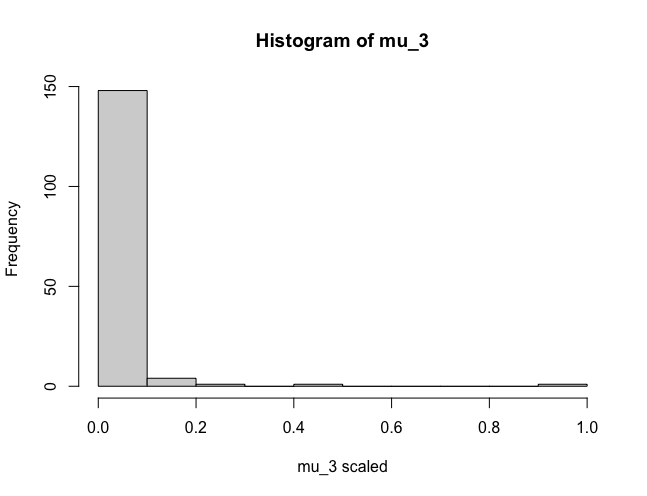
\includegraphics[width=8cm]{histogram_mu_3_scaled.png}
    \caption{Histogram of $\mu_3$ values for first time period for \textit{Twitter18}}
    \label{fig:Hist mu_3 Twitter18}
\end{figure}

This histogram is in line with all of the other analysis on epidemic spread previously discussed: every network is made up of many small nodes with a few large nodes. The average minmax-ed $\mu_3$ value was 0.04 and the median was 0.02. Most tweets are never retweeted and most have very limited engagement. Those tweets that are already fizzling out on their own do not need to be fact-checked, and this algorithm successfully identifies which have the highest current spread. 

Results for $\mu_4$ and $\mu_5$ (Fig. \ref{fig:Hist mu_4 Twitter18}):
\begin{figure}[h!]
    \centering
    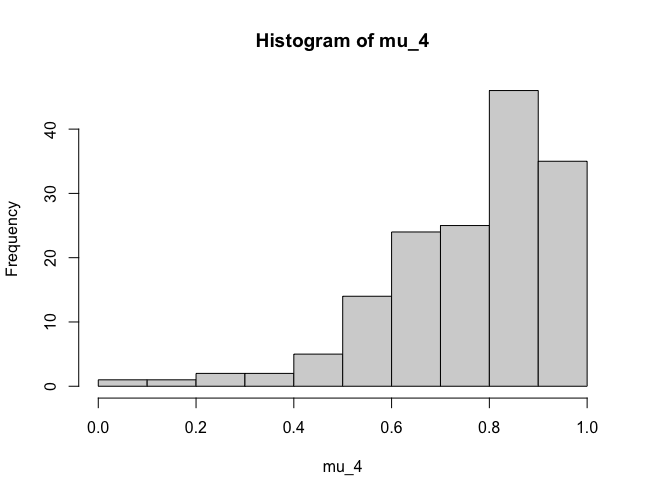
\includegraphics[width=8cm]{histogram of mu_4.png}
    \caption{Histogram of $\mu_4$ values for first time period for \textit{Twitter18}}
    \label{fig:Hist mu_4 Twitter18}
\end{figure}
As can be expected, the $\mu_4$ values skewed higher for $j=1$, since it is such a small time period, it takes very few retweets for $\lambda$ to appear unreasonably large.  

Results for $\mu_6$:
Because these tweets all "started" at the same time, $\mu_6$ was less informative than the other three. However, the $v_c$ value at $j=1$ was 0.89, which implies that around 89\% of all tweets need to be checked. 89\% is far too large of a number to consistently check as there are more than 500 million tweets per day \cite{raffi2013tweets}, which would require 445 million fact checks per day. That is unsustainable. However, it's important to recognize that 89\% is for \textbf{total} vaccination of the \textit{entire} network. That goal is neither desirable nor reachable. There is no need to slow the spread of positive or helpful content (e.g. coordination efforts during the Manchester bombing \cite{mirbabaie2020breaking, eriksson2016facebook}), only highly partisan and dangerous content. It is also important to recognize that, since $v_c \propto \langle \lambda \rangle$, as the tweets with a higher $\lambda$ value are removed, the average $\lambda$ value will decrease, which in turn provides a lower $v_c$ value.

In a real life scenario, a vaccinated high $\lambda$ post may be replaced with another high $\lambda$ post. At the same time, so long as those high $\lambda$ posts are fact-checked quickly, the $v_c$ value will continue to remain as low as possible. 

In this experiment, though, $\mu_6$ saw steady decrease in each time period (Fig. \ref{fig:mu6 Twitter18}), which implies that this algorithm did successfully remove the "super spreaders" first. In fact, when $j=1$, $\langle v_c \rangle = 0.894$, but by $j=24$, $\langle v_c \rangle = 0.091$. That is a substantial decrease.
\begin{figure}[h!]
    \centering
    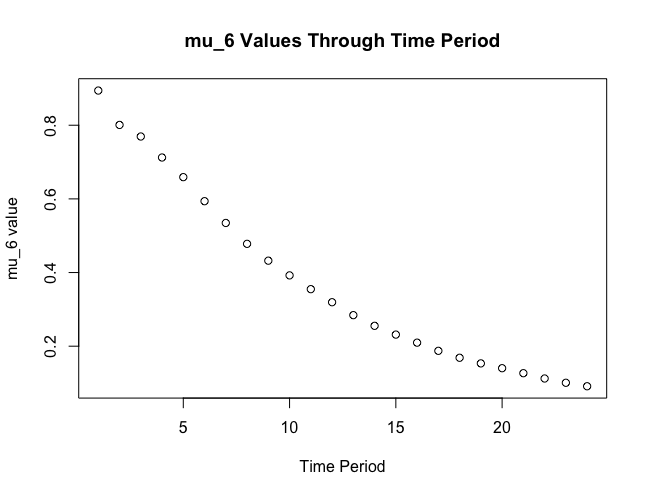
\includegraphics[width=8cm]{mu6 graph.png}
    \caption{Plot of $\mu_6$ values for each time period in \textit{Twitter18}}
    \label{fig:mu6 Twitter18}
\end{figure}
 

Results of the algorithm:
%\begin{longtable}[h]
%\centering
\begin{longtable}{ |p{0.5cm}|p{4.1cm}|p{12cm}|  }
\hline
\multicolumn{3}{|c|}{Algorithm Results} \\
\hline
$j$ & User & Tweet Text \\
\hline
1 & @deray & and @abc, please tweet saying that you did not pay or compensate darren wilson for the interview in any way. we're waiting. \#ferguson\\
\hline
2 & @realDonaldTrump & the fight against isis starts at our border. ‘at least’ 10 isis have been caught crossing the mexico border. build a wall!\\
\hline
3 & @realDonaldTrump & the first general killed in a combat zone since vietnam, it is a travesty that obama did not attend major general harold greene’s funeral\\
\hline
4 & @FoxNews & *Text Not Available. From a Suspended Account*\\
\hline
5 & @Lord\_Voldemort7 & once again, jk rowling is not working on an eighth harry potter book. i expect this rumour originated from either the quibbler or trelawney. \\
\hline
6 & @FoxNews & .@drzuhdijasser: "it's disgraceful that this is...the mosque that [@potus] picked to be the first visit." @ffweekend \\
\hline
7 & @FoxNews & boko haram burns kids alive in northeast nigeria, witness says \\
\hline
8 & @FoxNews & *Text Not Available. From a Suspended Account* \\
\hline
9 & @FoxNews & .@danaperino: "if i were in... legal trouble, i would call @hillaryclinton to find out how do you get out of it." \\
\hline
10 & @stephenfry & this is just about the weirdest fetish i've ever heard of. what was he thinking of? (via @elvis717) \\
\hline
11 & @HuffPost & no, internet, betty white is not dead \\
\hline
12 & @HuffPost & banksy shares simple but beautiful tribute to charlie hebdo cartoonists \\
\hline
13 & @HuffPost & michael jackson told oprah he doesn't want a white actor playing him in 1993\\
\hline
14 & @ndtv & first pics from the site in ukraine where \#mh17 crashed\\
\hline
15 & @HuffPost & gerrymandering is even more infuriating when you can actually see it \\
\hline
16 & @empiremagainze & he was severus snape. he was the sheriff of nottingham. he was alexander dane. he was, of course, hans gruber. we are devastated. \\
\hline
17 & @deray & y'all, i just read that abc paid darren wilson \$500k for the interview. destroying black life remains a lucrative american career. \#ferguson \\
\hline
18 & @jensan1332 & \#muslim arrested in \#texas today with \#isis flag on body armor \\
\hline
19 & @Complex & someone spray painted a penis on a \$2.4 million bugatti veyron \\
\hline
20 &@AlfredoFlores & i feel some type of way. \\
\hline
21 & @TMZ & stephen collins -- cops swarm home after suicide report ... false alarm \\
\hline
22 & @chrissyteigen & deep-fried left wings demo-crab cakes barack-amole \& chips malia quesadillas hawaiian pizza sloppy joe bidens obamacare-rot cake \\
\hline
23 & @BuzzFeed & breaking news: durex has not come out with a pumpkin spice condom \\
\hline
24 & @piersmorgan& breaking news: banksy not arrested, cover not blown. \\

\hline
\caption{Results of Algorithm on Twitter15 Set}
\label{Results of Algorithm Twitter15}
\end{longtable}

\subsubsection{Analysis}
Even setting $\langle \rho_{\Delta} \rangle$ to 0.5, highly partisan content still rose to the top of this list. 10 out of the 24 tweets that the algorithm selected are partisan in nature(Tweets 1, 2, 3, 4, 6, 8, 9, 15, 17, 18), 1 is clearly spam (Tweet 22), and 2 are news that need to be fact-checked (Tweets 7 and 14). Arguably, it is worthwhile for tweets surrounding celebrity deaths (Tweets 11, 16, and 21) to be fact-checked even though they aren't partisan in nature, since death hoaxes are a common source of fake news \cite{moses2017celebrity}.

It correctly vaccinated Tweet 1 first, as it had high values for $\mu_1$, $\mu_2$, $\mu_3$, and $\mu_4$: it came from a source with a high number of followers, focused on one of the top 10 bigrams (Darren Wilson was the officer who shot Michael Brown in Ferguson, MO \cite{halpern2015cop}), and was spreading quickly.The $v_c$ for this tweet at $j=1$ was 0.9959 -- almost every single node would have to be vaccinated or immunized in order to prevent this post from spreading. This charge by @deray is exactly the sort of tweet that should be checked first: it's on a controversial topic, it's \textit{sythetic a posteriori} knowledge, it's partisan, and could muddy the waters of discussion on the topic. 

This algorithm correctly vaccinated Tweet 5, since, even though it is not partisan in nature and not on an important topic, the number of users retweeting exceeded the number of followers very quickly. This implies an out-of-control virality, which should be checked.

This algorithm also correctly vaccinated Tweet 16. This tweet had the highest $\mu_3$ values for several of the previous time periods, but there was always a tweet with a higher $\zeta$ value, typically because of a much higher $\mu_1$ value. This is a situation where weighting the $\mu$ values would likely have provided different results, and tweet 16 may have been vaccinated earlier in the process, whereas tweet 13 may have been vaccinated later or not at all. 



\subsection{Twitter21}
TBD
\subsection{Stochastic21}
TBD

\section{Conclusion}
\subsection{Discussion}
The goal of this thesis was to provide a framework by which a fact checking team could maximize their resources and combat fake news in a scalable fashion. This solution has been provided. Unlike other fake news detection processes, it is adaptable to the user in question (Eq. \ref{mu_1 equation}), it factors in the importance of a topic on a given day (Eq. \ref{mu_2 equation}), it includes epidemic spreading rate of that particular tweet (Eq. \ref{mu_3 equation}), it de-prioritizs content at the end of its lifespan (Eq. \ref{mu_4 and mu_5}), and it provides a global KPI for the team to benchmark their successes (Eq. \ref{mu_4 and mu_5}).

From an epistemological standpoint, this thesis breaks down statements into various categories with assigned possible $\tau$ values, to separate content that machine learning is uniquely suited for and content that it is not. This is a stumbling block for global RNN solutions as they struggle with posts that are vague, hyperbolic, ironic, sarcastic, etc. This thesis makes no judgment about truth values, therefore there is no fear that an ironic statement will be deemed false. 

Visualizing this problem as an epidemic spread instead of a machine learning problem further allows for a recognition that not every node is susceptible to each particular strain of fake news (Eq. \ref{immunity equation}). It provides for the problem of echo-chambers (Sec. \ref{sec: echo chambers}) by factoring in partisanship into the Barab{\'a}si-Albert preferential attachment equation (Eq. \ref{Pdotpartisan}) and recognizing that highly partisan environments are breeding grounds for malicious actors. These issues of partisanship are included in $\tilde{\psi}$ and in the calculation of $u^*$'s. This allows for posts to be ranked according to communal susceptibility, whereas other solutions offer only blanket solutions based on text patterns and user information patterns. 

This solution is easily repeatable on a daily basis. By using moving averages for content with a half-life (Eqs. \ref{Finch Equations}), topics that were relevant last week but not this week fall off and are replaced by more significant topics. By including the moving variance as well, topics that have typically low volumes but then see large spikes, such as the preparation for the January 6th insurrection at the U.S. Capitol \cite{Levenson2021capitol}, would be caught by this metric. 

By not attempting to catch every error and fact-check every post, the resources here are maximized. Most tweets quickly reach a dead end and have no further spread; spending any time checking them is wasted effort. As seen in figure \ref{fig:mu6 Twitter18}, after "vaccinating" only 24 tweets from the data set, the remainder of the tweets had an extremely lower spread: at the beginning 89\% of the tweets would have to be removed to stop viral spread; at the end, only 10\% needed to be. It successfully identified the super-spreaders and targeted them first.

Finally, the resources required for this are far lower than those needed for an RNN that would attempt to check all of the 550 million tweets written per day. Many of these underlying numbers, such as $|\psi|$ values for each user, are relatively static and easily selected from the available data layers. The equations using those numbers are far less resource intensive than the perpetual training and implementation of a CNN or RNN. As mentioned in \ref{what is being shared summary}, yesterday's topics are not the same as today's topics; text/user patterns that the neural networks detected yesterday are easily changed today. That will require constant training, which will be heavily resource intensive. This thesis solves that.

A supplementary solution to this algorithm would be an inclusion of an impartial "Supreme Court" for fake news on social media platforms. Individuals who believe their content has been incorrectly removed can appeal to a "Supreme Court" who can decide to reinstate the post if they concur that it was removed in error. This is already in practice in collaborative knowledge sharing communities, such as Wikipedia \cite{hara2016co}, and has successfully help arbitrate between strongly held opinions and empirically derived facts. 

\subsection{Next Steps}
The next steps for validating this algorithm would be to use a much larger data set on computers with more sophisticated resources. Every piece of coding for this thesis was performed on a 2020 MacBook Air with only 8GB of RAM. Server level machines would be able to run this exact same algorithm much faster, and would be able to process the $\approx 6,366$ tweets that are posted every second on average. 

After that iteration, the next step would be to determine the $\beta$ weights for each $\mu$ value. For this thesis, every $\mu$ value was transformed using minmax, which made every $\mu$ value equally important. After several iterations of this algorithm, it may be determined that $\mu_3$ is far more important than $\mu_2$ in determining if content needs to be flagged for analysis -- the inclusion of $\beta$ weights will allow for this observation and may be recalibrated on an iterative basis until the optimal values are discovered.


%% The Appendices part is started with the command \appendix;
%% appendix sections are then done as normal sections
\appendix

\section{Truth Values}
\label{truthvalue appendix}
\subsection{Analytic a Priori}
An \textit{analytic a priori} statement's truth value is "true by virtue of meanings and independent of fact" \cite{quine1951main}. 
For example, proposition 1: \begin{center}
    $P_1$: All triangles have three sides.
\end{center}
The predicate "having three sides" is contained within the meaning of the word "triangle". There is no need to observe a given triangle in order to know that it must have three sides.

For the purposes of this discussion, racial slurs and other such language shall be considered \textit{analytic a priori} hate speech, as there is no need to observe all racial slurs in order to know that they were created and used with hate speech as the intent. Hate speech are fundamentally false statements \cite{waldron2012harm}, which automatically mean $\tau = 0$ .

\subsection{Synthetic a Priori}
A \textit{synthetic a priori} statement is true if it is universally true, no experience is needed to confirm it, but it is also not definitional in nature:
\begin{center}
    $P_2$: The sum of two sides of a triangle are greater than the third side.
\end{center}
 
As with $P_1$, there is no need to measure every triangle in existence to confirm this statement is true, yet there is nothing contained in the definition of a triangle that implies this relationship between the three sides.

In this thesis, spam will be considered false \textit{synthetic a priori} statements. Naive-Bayes classifiers have been incredibly successful at detecting spam messages \cite{wang2010detecting,xu2019exploiting,ahmed2018detecting}, in large part because they consistently illustrate the same telltale signs of being spam: broken English, seemingly random URL links, etc. Therefore, \begin{center}
    $P_3$: Spam messages are unsolicited messages that feature broken English, random links, etc. \\
$P_4$: Unsolicited messages that meet the requirements of $P_3$ are not truthful.\\
$C$: Spam messages are not truthful.
\end{center}
 
This syllogism is logically valid even though there is nothing in the definition of the word "spam" that leads to a truth value. Therefor, spam messages may also be set to $\tau = 0$.


\subsection{Analytic a Posteriori}
A statement is \textit{analytic a posteriori} if it is true by virtue of its definition, but requires empirical evidence to discover it \cite{kripke1972naming}. Kripke gives the example of Venus being both the morning and evening star: \begin{center}
   $P_5$: Venus is the morning star.\\
$P_6$: Venus is the evening star.\\
$C$: The morning star is the evening star. 
\end{center}


While this statement is necessarily true based off of the definitions of "morning star" and "evening star", it can't be considered \textit{a priori} true, as Homer (12th century BCE) refers to the morning and evening stars as separate objects, and it isn't until Pythagoras (500 BCE) that it is a scientifically accepted fact that the morning and evening stars refer to the same object, Venus \cite{dunne1978voyage}.

Scientific information would largely fall into this category. Propositions such as: 
\begin{center}
    $P_7$: Water is H$_2$O.
\end{center} 
are necessarily true and definitionally true, but were not known since the start of time -- in the case of water, it was not formally known until Avogadro in 1811. Scientific conspiracies such as the Earth being flat, would therefore be examples of \textit{analytic a posteriori} misinformation, as the Earth being round is scientifically true and definitionally true, per Frege, as any complete definition of the Earth would have to imply that it was a round planet \cite{frege2003sense}. Scientific misinformation that is definitionally true can also be set to $\tau = 0$.

\subsection{Synthetic a Posteriori}
A statement is \textit{synthetic a posteriori} if its truth value is contingent upon experience and non-definitional in nature. Statements such as: \begin{center}
    $P_8$: John Adams and Thomas Jefferson both died on July 4th, 1826.
\end{center}

would be \textit{synthetic a posteriori} true statements, as they are objectively true, but there is nothing in the definition of "John Adams" or "Thomas Jefferson" that implies a death date. External verification is necessary in order to determine the truthfulness of the statement.

The majority of the statements that Wu et al. attempt to break into subgroups would all be considered \textit{sythentic a posteriori} statements here: rumors, legends, etc. may or may not be true, but require external validation in order to determine their truthfulness.

\subsection{Hyperbole, Sarcasm, and Irony}
\label{hyperbole}
Finally, hyperbole, sarcasm, and irony should be separated from our truth value set, as these are statements that are intentionally false to point to a greater underlying truth. 
Current literature on using NLP to decipher sarcasm and irony primarily revolves around unexpected word combinations \cite{barbieri2014modelling,buschmeier2014impact,ghosh2015sarcastic} or RoBERTa recurrent neural networks \cite{potamias2020transformer}, and they all examine publicly available data sets, namely the Riloff Twitter set \cite{riloff2013sarcasm}, the Pt{\'a}{\v{c}}ek Twitter set \cite{ptavcek2014sarcasm}, the Khodak Reddit set \cite{khodak2017large} and two "Semantic Evaluation Workshop Tasks" \cite{van2018semeval,ghosh2015semeval}. Many of these are able to generate quite high F1 scores, especially the RCNN-RoBERTa transformer proposed by Potomias, Siolas, and Stafylopatis, whose F1 score was consistently around 0.8 in each of the unique data sets. 

However, as Oprea and Magdy point out, tools that are successful in one data set struggle in other data sets. Models trained in the Riloff data set can generate an F1 score above 0.8, but those same models will generate an F1 score near 0.5 (which is the same as random guessing) when applied to the Pt{\'a}{\v{c}}ek set \cite{oprea2019exploring}. This implies there are extreme differences in how groups express and perceive irony/sarcasm/hyperbole. Those differences are beyond the scope of what RNNs and RCNNs can currently successfully grasp. Therefore an alternative solution to handling irony on a global level is necessary.
\subsection{Summary}
\label{truthvalueappendixsummary}
To summarize, with examples of misinformation according to each distinction (table \ref{tab:misinformationexamples}),
\begin{table}[htbp]
    \centering
    \begin{tabular}{ |p{3cm}|p{5cm}|p{5cm}|}
    \hline
    & Analytic & Synthetic\\
    \hline
    A Priori & Hate Speech & Spam\\
    \hline
    A Posteriori &  Scientific Misinformation  & General Misinformation\\
    \hline
    \end{tabular}
    \caption{Misinformation Examples of Analytic/Synthetic Distinctions}
    \label{tab:misinformationexamples}
\end{table}
in terms of truth values, $\tau$, \textit{a priori} and \textit{analytic} statements are binary, but \textit{synthetic a posteriori} sentences may have a range of truthfulness (such as being misleading, partially true, mostly true, etc.) (table \ref{tab:truthvalues}).

\begin{table}[h!]
\centering
\begin{tabular}{ |p{3cm}|p{5cm}|p{5cm}|}
 \hline
  & Analytic & Synthetic\\
 \hline
 A Priori & $\tau \in \mathbb{B}$ & $\tau \in \mathbb{B}$\\
 \hline
 A Posteriori &  $\tau \in \mathbb{B}$  & $\tau \in \mathbb{R} \ | \ 0 \leq \tau \leq 1$ \\
 \hline
\end{tabular}
\caption{Truth Values of Analytic/Synthetic Distinctions}
\label{tab:truthvalues}
\end{table}

These proposed distinctions better capture the breadth of misinformation than the previously provided definitions: as with Klein, it concurs that intentionality is not relevant in determining truth value; unlike Wu et al. or DiFonzo \& Bordia, it makes no distinction between types of misinformation such as "rumor" and "misinformation"; unlike Liu \& Wu, it separates hate speech, spam, and scientific misinformation from generalized misinformation; unlike all other examples, it includes sarcasm, hyperbole, and irony. 

\newpage
\bibliographystyle{elsarticle-num-names} 
\bibliography{bibliography}


\end{document}

\endinput

